%%=============================================================================
%% LaTeX sjabloon voor bachelorproef, HoGent Bedrijf en Organisatie
%% Opleiding Toegepaste Informatica
%%=============================================================================

\documentclass[fleqn,a4paper,12pt]{book}

%%=============================================================================
%% LaTeX sjabloon voor de bachelorproef, HoGent Bedrijf en Organisatie
%% Opleiding toegepaste informatica
%%
%% Structuur en algemene vormgeving. Meestal hoef je hier niets te wijzigen.
%%
%% Vormgeving gebaseerd op "The Legrand Orange Book", version 2.0 (9/2/15)
%% door Mathias Legrand (legrand.mathias@gmail.com) met aanpassingen door
%% Vel (vel@latextemplates.com). Het oorspronkelijke template is te vinden op
%% http://www.LaTeXTemplates.com
%%
%% Aanpassingen voor HoGent toegepaste informatica: 
%%   Bert Van Vreckem <bert.vanvreckem@hogent.be>
%% Licentie: 
%%   CC BY-NC-SA 3.0 (http://creativecommons.org/licenses/by-nc-sa/3.0/)
%%=============================================================================

%%-----------------------------------------------------------------------------
%% Packages
%%-----------------------------------------------------------------------------

\usepackage[top=3cm,bottom=3cm,left=3cm,right=3cm,headsep=10pt,a4paper]{geometry} % Page margins
\usepackage[utf8]{inputenc}  % Accenten gebruiken in tekst (vb. é ipv \'e)
\usepackage{amsfonts}        % AMS math packages: extra wiskundige
\usepackage{amsmath}         %   symbolen (o.a. getallen-
\usepackage{amssymb}         %   verzamelingen N, R, Z, Q, etc.)
\usepackage[english,dutch]{babel}    % Taalinstellingen: woordsplitsingen,
                             %  commando's voor speciale karakters
                             %  ("dutch" voor NL)
\usepackage{iflang}
\usepackage{eurosym}         % Euro-symbool €
\usepackage{geometry}
\usepackage{graphicx}        % Invoegen van tekeningen
\graphicspath{{img/}}       % Specifies the directory where pictures are stored
\usepackage{tikz}            % Required for drawing custom shapes
\usepackage[pdftex,bookmarks=true]{hyperref}
                             % PDF krijgt klikbare links & verwijzingen,
                             %  inhoudstafel
\usepackage{enumitem}        % Customize lists
\setlist{nolistsep}         % Reduce spacing between list items
\usepackage{listings}        % Broncode mooi opmaken
\usepackage{multirow}        % Tekst over verschillende cellen in tabellen
\usepackage{rotating}        % Tabellen en figuren roteren

\usepackage{booktabs}        % Required for nicer horizontal rules in tables

\usepackage{xcolor}          % Required for specifying colors by name
\definecolor{maincolor}{RGB}{0,147,208} % Define the main color used for 
                             % highlighting throughout the book
                             % 0, 147, 208 = officiële kleur HoGent FBO

% Paragraph style: no indent, add space between paragraphs
\setlength{\parindent}{0em}
\setlength{\parskip}{1em}

\usepackage{etoolbox}
\usepackage{titling} % Macros for title, author, etc
\usepackage{lipsum}          % Voor vultekst (lorem ipsum)

%----------------------------------------------------------------------------------------
%	FONTS
%----------------------------------------------------------------------------------------

\usepackage{avant} % Use the Avantgarde font for headings
%\usepackage{times} % Use the Times font for headings
\usepackage{mathptmx} % Use the Adobe Times Roman as the default text font together with math symbols from the Sym­bol, Chancery and Com­puter Modern fonts

\usepackage{microtype} % Slightly tweak font spacing for aesthetics
\usepackage[utf8]{inputenc} % Required for including letters with accents
\usepackage[T1]{fontenc} % Use 8-bit encoding that has 256 glyphs

%------------------------------------------------------------------------------
%	TITLE PAGE
%------------------------------------------------------------------------------

\newcommand{\inserttitlepage}{%
\begin{titlepage}
  \newgeometry{top=2cm,bottom=1.5cm,left=1.5cm,right=1.5cm}
  \begin{center}

    \begingroup
    \rmfamily
    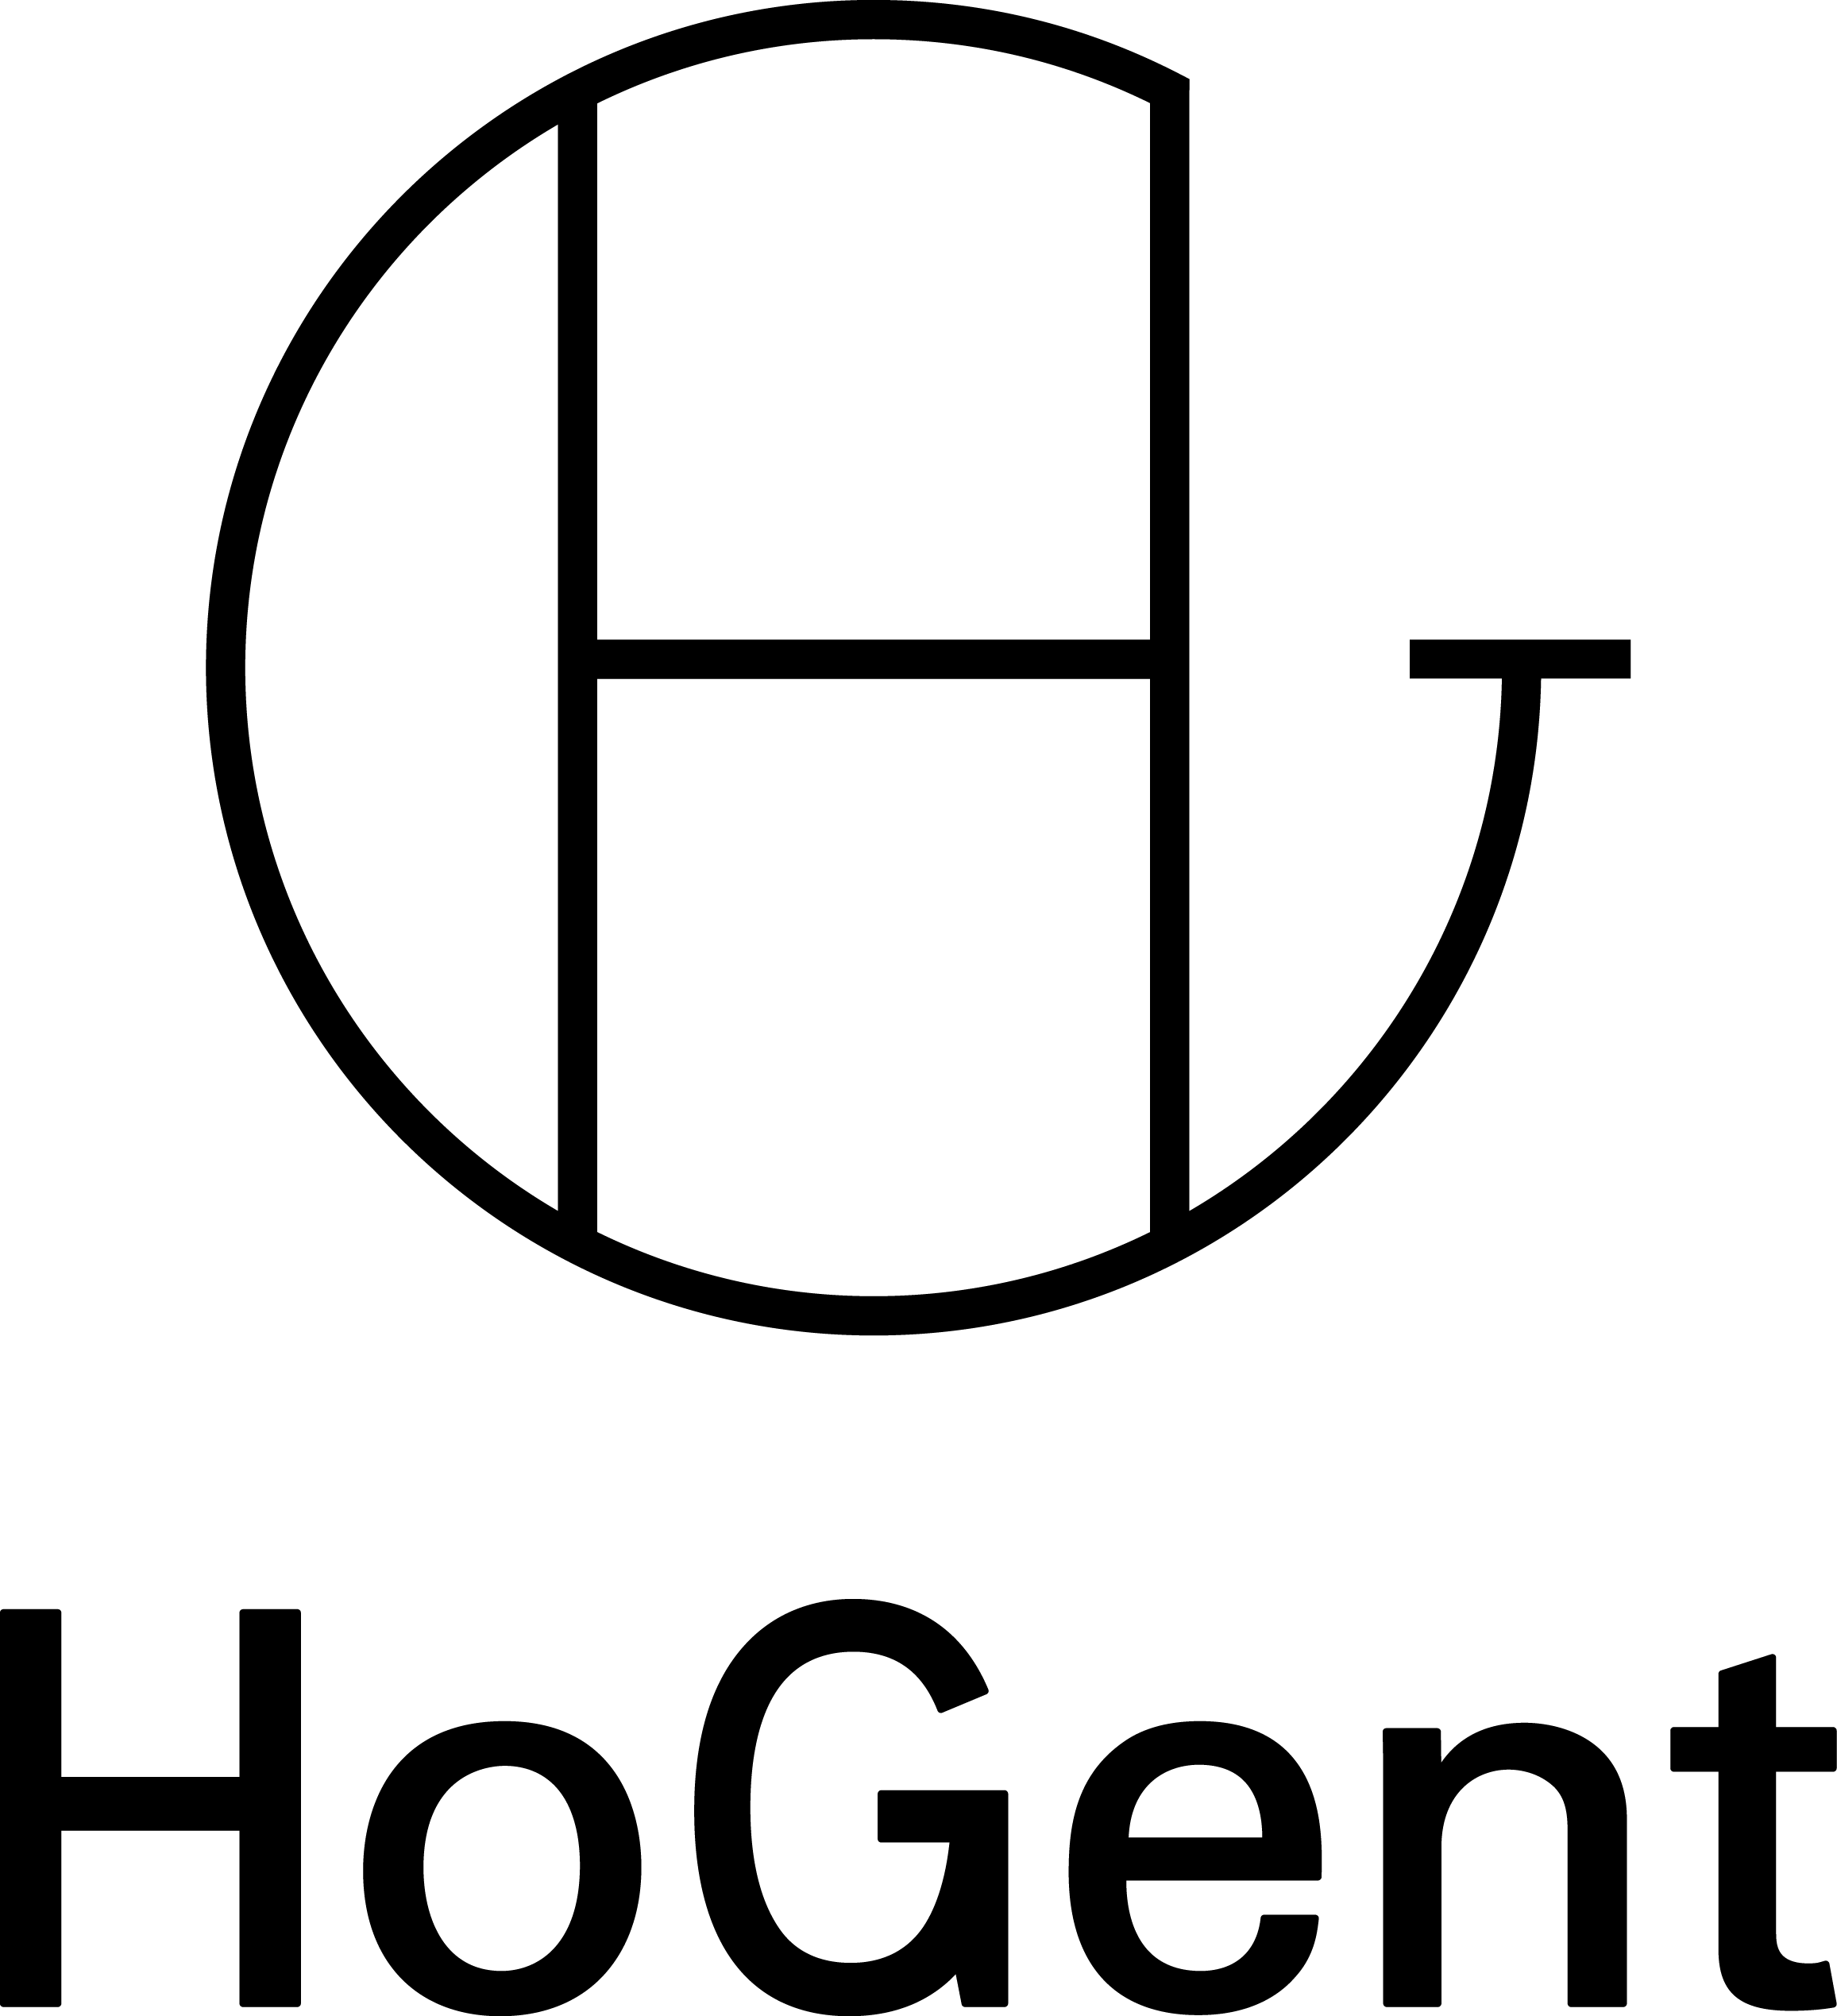
\includegraphics[width=2.5cm]{img/HG-beeldmerk-woordmerk}\\[.5cm]
    Faculteit Bedrijf en Organisatie\\[3cm]
    \titel
    \vfill
    \student\\[3.5cm]
    Scriptie voorgedragen tot het bekomen van de graad van\\professionele bachelor in de toegepaste informatica\\[2cm]
    Promotor:\\
    \promotor\\
    \ifdefempty{\copromotor}{\vspace{2.5cm}}{Co-promotor:\\\copromotor\\[2.5cm]}
    Instelling: \instelling\\[.5cm]
    Academiejaar: \academiejaar\\[.5cm]
    \ifcase \examenperiode \or Eerste \or Tweede \else Derde \fi examenperiode
    \endgroup

  \end{center}
  \restoregeometry
\end{titlepage}
  \emptypage
\begin{titlepage}
  \newgeometry{top=5.35cm,bottom=1.5cm,left=1.5cm,right=1.5cm}
  \begin{center}

    \begingroup
    \rmfamily
    \IfLanguageName{dutch}{Faculteit Bedrijf en Organisatie}{Faculty of Business and Information Management}\\[3cm]
    \titel
    \vfill
    \student\\[3.5cm]
    \IfLanguageName{dutch}{Scriptie voorgedragen tot het bekomen van de graad van\\professionele bachelor in de toegepaste informatica}{Thesis submitted in partial fulfilment of the requirements for the degree of\\professional bachelor of applied computer science}\\[2cm]
    Promotor:\\
    \promotor\\
    \ifdefempty{\copromotor}{\vspace{2.5cm}}{Co-promotor:\\\copromotor\\[2.5cm]}
    \IfLanguageName{dutch}{Instelling}{Institution}: \instelling\\[.5cm]
    \IfLanguageName{dutch}{Academiejaar}{Academic year}: \academiejaar\\[.5cm]
    \IfLanguageName{dutch}{%
    \ifcase \examenperiode \or Eerste \or Tweede \else Derde \fi examenperiode}{%
    \ifcase \examenperiode \or First \or Second \else Third \fi examination period}
    \endgroup

  \end{center}
  \restoregeometry
\end{titlepage}
}

%----------------------------------------------------------------------------------------
%	BIBLIOGRAPHY AND INDEX
%----------------------------------------------------------------------------------------

\usepackage[style=apa,backend=biber]{biblatex}
%\usepackage{apacite}
\usepackage{csquotes}
\DeclareLanguageMapping{dutch}{dutch-apa}
\addbibresource{bachproef-tin.bib} % BibTeX bibliography file
\addbibresource{voorstel/voorstel.bib}
\defbibheading{bibempty}{}

\usepackage{calc} % For simpler calculation - used for spacing the index letter headings correctly
\usepackage{makeidx} % Required to make an index
\makeindex % Tells LaTeX to create the files required for indexing
\usepackage[acronym]{glossaries}
\makeglossaries
%----------------------------------------------------------------------------------------
%	MAIN TABLE OF CONTENTS
%----------------------------------------------------------------------------------------

\usepackage{titletoc} % Required for manipulating the table of contents

\contentsmargin{0cm} % Removes the default margin

% Part text styling
\titlecontents{part}[0cm]
{\addvspace{20pt}\centering\large\bfseries}
{}
{}
{}

% Chapter text styling
\titlecontents{chapter}[1.25cm] % Indentation
{\addvspace{12pt}\large\sffamily\bfseries} % Spacing and font options for chapters
{\color{maincolor!60}\contentslabel[\Large\thecontentslabel]{1.25cm}\color{maincolor}} % Chapter number
{\color{maincolor}}
{\color{maincolor!60}\normalsize\;\titlerule*[.5pc]{.}\;\thecontentspage} % Page number

% Section text styling
\titlecontents{section}[1.25cm] % Indentation
{\addvspace{3pt}\sffamily\bfseries} % Spacing and font options for sections
{\contentslabel[\thecontentslabel]{1.25cm}} % Section number
{}
{\hfill\color{black}\thecontentspage} % Page number
[]

% Subsection text styling
\titlecontents{subsection}[1.25cm] % Indentation
{\addvspace{1pt}\sffamily\small} % Spacing and font options for subsections
{\contentslabel[\thecontentslabel]{1.25cm}} % Subsection number
{}
{\ \titlerule*[.5pc]{.}\;\thecontentspage} % Page number
[]

% List of figures
\titlecontents{figure}[0em]
{\addvspace{-5pt}\sffamily}
{\thecontentslabel\hspace*{1em}}
{}
{\ \titlerule*[.5pc]{.}\;\thecontentspage}
[]

% List of tables
\titlecontents{table}[0em]
{\addvspace{-5pt}\sffamily}
{\thecontentslabel\hspace*{1em}}
{}
{\ \titlerule*[.5pc]{.}\;\thecontentspage}
[]

%----------------------------------------------------------------------------------------
%	MINI TABLE OF CONTENTS IN PART HEADS
%----------------------------------------------------------------------------------------

% Chapter text styling
\titlecontents{lchapter}[0em] % Indenting
{\addvspace{15pt}\large\sffamily\bfseries} % Spacing and font options for chapters
{\color{maincolor}\contentslabel[\Large\thecontentslabel]{1.25cm}\color{maincolor}} % Chapter number
{}
{\color{maincolor}\normalsize\sffamily\bfseries\;\titlerule*[.5pc]{.}\;\thecontentspage} % Page number

% Section text styling
\titlecontents{lsection}[0em] % Indenting
{\sffamily\small} % Spacing and font options for sections
{\contentslabel[\thecontentslabel]{1.25cm}} % Section number
{}
{}

% Subsection text styling
\titlecontents{lsubsection}[.5em] % Indentation
{\normalfont\footnotesize\sffamily} % Font settings
{}
{}
{}

%----------------------------------------------------------------------------------------
%	PAGE HEADERS
%----------------------------------------------------------------------------------------

\usepackage{fancyhdr} % Required for header and footer configuration

\pagestyle{fancy}
\renewcommand{\chaptermark}[1]{\markboth{\sffamily\normalsize\bfseries\chaptername\ \thechapter.\ #1}{}} % Chapter text font settings
\renewcommand{\sectionmark}[1]{\markright{\sffamily\normalsize\thesection\hspace{5pt}#1}{}} % Section text font settings
\fancyhf{} \fancyhead[LE,RO]{\sffamily\normalsize\thepage} % Font setting for the page number in the header
\fancyhead[LO]{\rightmark} % Print the nearest section name on the left side of odd pages
\fancyhead[RE]{\leftmark} % Print the current chapter name on the right side of even pages
\renewcommand{\headrulewidth}{0.5pt} % Width of the rule under the header
\addtolength{\headheight}{2.5pt} % Increase the spacing around the header slightly
\renewcommand{\footrulewidth}{0pt} % Removes the rule in the footer
\fancypagestyle{plain}{\fancyhead{}\renewcommand{\headrulewidth}{0pt}} % Style for when a plain pagestyle is specified

% Removes the header from odd empty pages at the end of chapters
\makeatletter
\renewcommand{\cleardoublepage}{
\clearpage\ifodd\c@page\else
\hbox{}
\vspace*{\fill}
\thispagestyle{empty}
\newpage
\fi}

%----------------------------------------------------------------------------------------
%	THEOREM STYLES
%----------------------------------------------------------------------------------------

\usepackage{amsmath,amsfonts,amssymb,amsthm} % For math equations, theorems, symbols, etc

\newcommand{\intoo}[2]{\mathopen{]}#1\,;#2\mathclose{[}}
\newcommand{\ud}{\mathop{\mathrm{{}d}}\mathopen{}}
\newcommand{\intff}[2]{\mathopen{[}#1\,;#2\mathclose{]}}
\newtheorem{notation}{Notation}[chapter]

% Boxed/framed environments
\newtheoremstyle{maincolornumbox}% % Theorem style name
{0pt}% Space above
{0pt}% Space below
{\normalfont}% % Body font
{}% Indent amount
{\small\bf\sffamily\color{maincolor}}% % Theorem head font
{\;}% Punctuation after theorem head
{0.25em}% Space after theorem head
{\small\sffamily\color{maincolor}\thmname{#1}\nobreakspace\thmnumber{\@ifnotempty{#1}{}\@upn{#2}}% Theorem text (e.g. Theorem 2.1)
\thmnote{\nobreakspace\the\thm@notefont\sffamily\bfseries\color{black}---\nobreakspace#3.}} % Optional theorem note
\renewcommand{\qedsymbol}{$\blacksquare$}% Optional qed square

\newtheoremstyle{blacknumex}% Theorem style name
{5pt}% Space above
{5pt}% Space below
{\normalfont}% Body font
{} % Indent amount
{\small\bf\sffamily}% Theorem head font
{\;}% Punctuation after theorem head
{0.25em}% Space after theorem head
{\small\sffamily{\tiny\ensuremath{\blacksquare}}\nobreakspace\thmname{#1}\nobreakspace\thmnumber{\@ifnotempty{#1}{}\@upn{#2}}% Theorem text (e.g. Theorem 2.1)
\thmnote{\nobreakspace\the\thm@notefont\sffamily\bfseries---\nobreakspace#3.}}% Optional theorem note

\newtheoremstyle{blacknumbox} % Theorem style name
{0pt}% Space above
{0pt}% Space below
{\normalfont}% Body font
{}% Indent amount
{\small\bf\sffamily}% Theorem head font
{\;}% Punctuation after theorem head
{0.25em}% Space after theorem head
{\small\sffamily\thmname{#1}\nobreakspace\thmnumber{\@ifnotempty{#1}{}\@upn{#2}}% Theorem text (e.g. Theorem 2.1)
\thmnote{\nobreakspace\the\thm@notefont\sffamily\bfseries---\nobreakspace#3.}}% Optional theorem note

% Non-boxed/non-framed environments
\newtheoremstyle{maincolornum}% % Theorem style name
{5pt}% Space above
{5pt}% Space below
{\normalfont}% % Body font
{}% Indent amount
{\small\bf\sffamily\color{maincolor}}% % Theorem head font
{\;}% Punctuation after theorem head
{0.25em}% Space after theorem head
{\small\sffamily\color{maincolor}\thmname{#1}\nobreakspace\thmnumber{\@ifnotempty{#1}{}\@upn{#2}}% Theorem text (e.g. Theorem 2.1)
\thmnote{\nobreakspace\the\thm@notefont\sffamily\bfseries\color{black}---\nobreakspace#3.}} % Optional theorem note
\renewcommand{\qedsymbol}{$\blacksquare$}% Optional qed square
\makeatother

% Defines the theorem text style for each type of theorem to one of the three styles above
\newcounter{dummy}
\numberwithin{dummy}{section}
\theoremstyle{maincolornumbox}
\newtheorem{theoremeT}[dummy]{Theorem}
\newtheorem{problem}{Problem}[chapter]
\newtheorem{exerciseT}{Exercise}[chapter]
\theoremstyle{blacknumex}
\newtheorem{exampleT}{Example}[chapter]
\theoremstyle{blacknumbox}
\newtheorem{vocabulary}{Vocabulary}[chapter]
\newtheorem{definitionT}{Definition}[section]
\newtheorem{corollaryT}[dummy]{Corollary}
\theoremstyle{maincolornum}
\newtheorem{proposition}[dummy]{Proposition}

%----------------------------------------------------------------------------------------
%	DEFINITION OF COLORED BOXES
%----------------------------------------------------------------------------------------

\RequirePackage[framemethod=default]{mdframed} % Required for creating the theorem, definition, exercise and corollary boxes

% Theorem box
\newmdenv[skipabove=7pt,
skipbelow=7pt,
backgroundcolor=black!5,
linecolor=maincolor,
innerleftmargin=5pt,
innerrightmargin=5pt,
innertopmargin=5pt,
leftmargin=0cm,
rightmargin=0cm,
innerbottommargin=5pt]{tBox}

% Exercise box
\newmdenv[skipabove=7pt,
skipbelow=7pt,
rightline=false,
leftline=true,
topline=false,
bottomline=false,
backgroundcolor=maincolor!10,
linecolor=maincolor,
innerleftmargin=5pt,
innerrightmargin=5pt,
innertopmargin=5pt,
innerbottommargin=5pt,
leftmargin=0cm,
rightmargin=0cm,
linewidth=4pt]{eBox}

% Definition box
\newmdenv[skipabove=7pt,
skipbelow=7pt,
rightline=false,
leftline=true,
topline=false,
bottomline=false,
linecolor=maincolor,
innerleftmargin=5pt,
innerrightmargin=5pt,
innertopmargin=0pt,
leftmargin=0cm,
rightmargin=0cm,
linewidth=4pt,
innerbottommargin=0pt]{dBox}

% Corollary box
\newmdenv[skipabove=7pt,
skipbelow=7pt,
rightline=false,
leftline=true,
topline=false,
bottomline=false,
linecolor=gray,
backgroundcolor=black!5,
innerleftmargin=5pt,
innerrightmargin=5pt,
innertopmargin=5pt,
leftmargin=0cm,
rightmargin=0cm,
linewidth=4pt,
innerbottommargin=5pt]{cBox}

% Creates an environment for each type of theorem and assigns it a theorem text style from the "Theorem Styles" section above and a colored box from above
\newenvironment{theorem}{\begin{tBox}\begin{theoremeT}}{\end{theoremeT}\end{tBox}}
\newenvironment{exercise}{\begin{eBox}\begin{exerciseT}}{\hfill{\color{maincolor}\tiny\ensuremath{\blacksquare}}\end{exerciseT}\end{eBox}}
\newenvironment{definition}{\begin{dBox}\begin{definitionT}}{\end{definitionT}\end{dBox}}
\newenvironment{example}{\begin{exampleT}}{\hfill{\tiny\ensuremath{\blacksquare}}\end{exampleT}}
\newenvironment{corollary}{\begin{cBox}\begin{corollaryT}}{\end{corollaryT}\end{cBox}}

%----------------------------------------------------------------------------------------
%	REMARK ENVIRONMENT
%----------------------------------------------------------------------------------------

\newenvironment{remark}{\par\vspace{10pt}\small % Vertical white space above the remark and smaller font size
\begin{list}{}{
\leftmargin=35pt % Indentation on the left
\rightmargin=25pt}\item\ignorespaces % Indentation on the right
\makebox[-2.5pt]{\begin{tikzpicture}[overlay]
\node[draw=maincolor!60,line width=1pt,circle,fill=maincolor!25,font=\sffamily\bfseries,inner sep=2pt,outer sep=0pt] at (-15pt,0pt){\textcolor{maincolor}{R}};\end{tikzpicture}} % Orange R in a circle
\advance\baselineskip -1pt}{\end{list}\vskip5pt} % Tighter line spacing and white space after remark

%----------------------------------------------------------------------------------------
%	SECTION NUMBERING IN THE MARGIN
%----------------------------------------------------------------------------------------

\makeatletter
\renewcommand{\@seccntformat}[1]{\llap{\textcolor{maincolor}{\csname the#1\endcsname}\hspace{1em}}}
\renewcommand{\section}{\@startsection{section}{1}{\z@}
{-4ex \@plus -1ex \@minus -.4ex}
{1ex \@plus.2ex }
{\normalfont\large\sffamily\bfseries}}
\renewcommand{\subsection}{\@startsection {subsection}{2}{\z@}
{-3ex \@plus -0.1ex \@minus -.4ex}
{0.5ex \@plus.2ex }
{\normalfont\sffamily\bfseries}}
\renewcommand{\subsubsection}{\@startsection {subsubsection}{3}{\z@}
{-2ex \@plus -0.1ex \@minus -.2ex}
{.2ex \@plus.2ex }
{\normalfont\small\sffamily\bfseries}}
\renewcommand\paragraph{\@startsection{paragraph}{4}{\z@}
{-2ex \@plus-.2ex \@minus .2ex}
{.1ex}
{\normalfont\small\sffamily\bfseries}}

%----------------------------------------------------------------------------------------
%	PART HEADINGS
%----------------------------------------------------------------------------------------

% numbered part in the table of contents
\newcommand{\@mypartnumtocformat}[2]{%
\setlength\fboxsep{0pt}%
\noindent\colorbox{maincolor!20}{\strut\parbox[c][.7cm]{\ecart}{\color{maincolor!70}\Large\sffamily\bfseries\centering#1}}\hskip\esp\colorbox{maincolor!40}{\strut\parbox[c][.7cm]{\linewidth-\ecart-\esp}{\Large\sffamily\centering#2}}}%
%%%%%%%%%%%%%%%%%%%%%%%%%%%%%%%%%%
% unnumbered part in the table of contents
\newcommand{\@myparttocformat}[1]{%
\setlength\fboxsep{0pt}%
\noindent\colorbox{maincolor!40}{\strut\parbox[c][.7cm]{\linewidth}{\Large\sffamily\centering#1}}}%
%%%%%%%%%%%%%%%%%%%%%%%%%%%%%%%%%%
\newlength\esp
\setlength\esp{4pt}
\newlength\ecart
\setlength\ecart{1.2cm-\esp}
\newcommand{\thepartimage}{}%
\newcommand{\partimage}[1]{\renewcommand{\thepartimage}{#1}}%
\def\@part[#1]#2{%
\ifnum \c@secnumdepth >-2\relax%
\refstepcounter{part}%
\addcontentsline{toc}{part}{\texorpdfstring{\protect\@mypartnumtocformat{\thepart}{#1}}{\partname~\thepart\ ---\ #1}}
\else%
\addcontentsline{toc}{part}{\texorpdfstring{\protect\@myparttocformat{#1}}{#1}}%
\fi%
\startcontents%
\markboth{}{}%
{\thispagestyle{empty}%
\begin{tikzpicture}[remember picture,overlay]%
\node at (current page.north west){\begin{tikzpicture}[remember picture,overlay]%
\fill[maincolor!20](0cm,0cm) rectangle (\paperwidth,-\paperheight);
\node[anchor=north] at (4cm,-3.25cm){\color{maincolor!40}\fontsize{220}{100}\sffamily\bfseries\@Roman\c@part};
\node[anchor=south east] at (\paperwidth-1cm,-\paperheight+1cm){\parbox[t][][t]{8.5cm}{
\printcontents{l}{0}{\setcounter{tocdepth}{1}}%
}};
\node[anchor=north east] at (\paperwidth-1.5cm,-3.25cm){\parbox[t][][t]{15cm}{\strut\raggedleft\color{white}\fontsize{30}{30}\sffamily\bfseries#2}};
\end{tikzpicture}};
\end{tikzpicture}}%
\@endpart}
\def\@spart#1{%
\startcontents%
\phantomsection
{\thispagestyle{empty}%
\begin{tikzpicture}[remember picture,overlay]%
\node at (current page.north west){\begin{tikzpicture}[remember picture,overlay]%
\fill[maincolor!20](0cm,0cm) rectangle (\paperwidth,-\paperheight);
\node[anchor=north east] at (\paperwidth-1.5cm,-3.25cm){\parbox[t][][t]{15cm}{\strut\raggedleft\color{white}\fontsize{30}{30}\sffamily\bfseries#1}};
\end{tikzpicture}};
\end{tikzpicture}}
\addcontentsline{toc}{part}{\texorpdfstring{%
\setlength\fboxsep{0pt}%
\noindent\protect\colorbox{maincolor!40}{\strut\protect\parbox[c][.7cm]{\linewidth}{\Large\sffamily\protect\centering #1\quad\mbox{}}}}{#1}}%
\@endpart}
\def\@endpart{\vfil\newpage
\if@twoside
\if@openright
\null
\thispagestyle{empty}%
\newpage
\fi
\fi
\if@tempswa
\twocolumn
\fi}

%----------------------------------------------------------------------------------------
%	CHAPTER HEADINGS
%----------------------------------------------------------------------------------------

% A switch to conditionally include a picture, implemented by  Christian Hupfer
\newif\ifusechapterimage
\usechapterimagetrue
\newcommand{\thechapterimage}{}%
\newcommand{\chapterimage}[1]{\ifusechapterimage\renewcommand{\thechapterimage}{#1}\fi}%
\def\@makechapterhead#1{%
{\parindent \z@ \raggedright \normalfont
\ifnum \c@secnumdepth >\m@ne
\if@mainmatter
\begin{tikzpicture}[remember picture,overlay]
\node at (current page.north west)
{\begin{tikzpicture}[remember picture,overlay]
\node[anchor=north west,inner sep=0pt] at (0,0) {\ifusechapterimage\includegraphics[width=\paperwidth]{\thechapterimage}\fi};
\draw[anchor=west] (\Gm@lmargin,-9cm) node [line width=2pt,rounded corners=15pt,draw=maincolor,fill=white,fill opacity=0.5,inner sep=15pt]{\strut\makebox[22cm]{}};
\draw[anchor=west] (\Gm@lmargin+.3cm,-9cm) node {\huge\sffamily\bfseries\color{black}\thechapter. #1\strut};
\end{tikzpicture}};
\end{tikzpicture}
\else
\begin{tikzpicture}[remember picture,overlay]
\node at (current page.north west)
{\begin{tikzpicture}[remember picture,overlay]
\node[anchor=north west,inner sep=0pt] at (0,0) {\ifusechapterimage\includegraphics[width=\paperwidth]{\thechapterimage}\fi};
\draw[anchor=west] (\Gm@lmargin,-9cm) node [line width=2pt,rounded corners=15pt,draw=maincolor,fill=white,fill opacity=0.5,inner sep=15pt]{\strut\makebox[22cm]{}};
\draw[anchor=west] (\Gm@lmargin+.3cm,-9cm) node {\huge\sffamily\bfseries\color{black}#1\strut};
\end{tikzpicture}};
\end{tikzpicture}
\fi\fi\par\vspace*{270\p@}}}

%-------------------------------------------

\def\@makeschapterhead#1{%
\begin{tikzpicture}[remember picture,overlay]
\node at (current page.north west)
{\begin{tikzpicture}[remember picture,overlay]
\node[anchor=north west,inner sep=0pt] at (0,0) {\ifusechapterimage\includegraphics[width=\paperwidth]{\thechapterimage}\fi};
\draw[anchor=west] (\Gm@lmargin,-9cm) node [line width=2pt,rounded corners=15pt,draw=maincolor,fill=white,fill opacity=0.5,inner sep=15pt]{\strut\makebox[22cm]{}};
\draw[anchor=west] (\Gm@lmargin+.3cm,-9cm) node {\huge\sffamily\bfseries\color{black}#1\strut};
\end{tikzpicture}};
\end{tikzpicture}
\par\vspace*{270\p@}}
\makeatother

%----------------------------------------------------------------------------------------
%	HYPERLINKS IN THE DOCUMENTS
%----------------------------------------------------------------------------------------

\usepackage{hyperref}
\hypersetup{hidelinks,colorlinks=false,breaklinks=true,urlcolor= maincolor,bookmarksopen=false,pdftitle={Title},pdfauthor={Author}}
\usepackage{bookmark}
\bookmarksetup{
open,
numbered,
addtohook={%
\ifnum\bookmarkget{level}=0 % chapter
\bookmarksetup{bold}%
\fi
\ifnum\bookmarkget{level}=-1 % part
\bookmarksetup{color=maincolor,bold}%
\fi
}
}

%----------------------------------------------------------------------------------------
%	Java source code
%----------------------------------------------------------------------------------------

% Commando voor invoegen Java-broncodebestanden (dank aan Niels Corneille)
% Gebruik:
%   \codefragment{source/MijnKlasse.java}{Uitleg bij de code}
%
% Je kan dit aanpassen aan de taal die je zelf het meeste gebruikt in je
% bachelorproef.
\usepackage{color}
\definecolor{lightgray}{rgb}{0.95, 0.95, 0.95}
\definecolor{darkgray}{rgb}{0.4, 0.4, 0.4}
%\definecolor{purple}{rgb}{0.65, 0.12, 0.82}
\definecolor{editorGray}{rgb}{0.95, 0.95, 0.95}
\definecolor{editorOcher}{rgb}{1, 0.5, 0} % #FF7F00 -> rgb(239, 169, 0)
\definecolor{editorGreen}{rgb}{0, 0.5, 0} % #007C00 -> rgb(0, 124, 0)
\definecolor{orange}{rgb}{1,0.45,0.13}		
\definecolor{olive}{rgb}{0.17,0.59,0.20}
\definecolor{brown}{rgb}{0.69,0.31,0.31}
\definecolor{purple}{rgb}{0.38,0.18,0.81}
\definecolor{lightblue}{rgb}{0.1,0.57,0.7}
\definecolor{lightred}{rgb}{1,0.4,0.5}

\lstdefinelanguage{JavaScript}{
  keywords={describe, await, async, const, typeof, new, true, false, catch, function, return, null, catch, switch, var, if, in, while, do, else, case, break, exports.config, module.exports, before:, before, browser, after:, after, exports.command, break, for},
  ndkeywords={default, expect, textContent, setData, port:, port, path:, specs:, exclude:, maxInstances:, capabilities:, sync:, logLevel:, coloredLogs:, deprecationWarnings:, bail:, screenshotPath:, baseUrl:, waitforTimeout:, connectionRetryTimeout:, connectionRetryCount:, framework:, mochaOpts:, ui:, services:, chromeDriverArgs:, chromeDriverLogs:, chromedriver, exports, url, assert.containsText, setValue, submitForm, useXpath, end, useCss, click, assert.containsText, submitForm, require, adminUsername:, adminPassword:, timeoutTime:, launch\_url:, env:, chromeDesktop:, chromeHeadless:, firefoxDesktop:, firefoxHeadless:, drupalAssertParagraphButton,
drupalAssertParagraphCkeditor,
drupalAssertParagraphFaq,
drupalAssertParagraphForm,
drupalAssertParagraphGuidance,
drupalAssertParagraphImage,
drupalAssertParagraphLink,
drupalAssertParagraphTestimonial,
drupalAssertParagraphTitle,
drupalAssertParagraphUsp,
drupalAssertParagraphVideo,
drupalAssertParagraphViewmode,
drupalCreatePageWithParagraph,
drupalDeletePage,
drupalInputParagraphButton,
drupalInputParagraphCkeditor,
drupalInputParagraphFaq,
drupalInputParagraphForm,
drupalInputParagraphGuidance,
drupalInputParagraphImage,
drupalInputParagraphLink,
drupalInputParagraphTestimonial,
drupalInputParagraphTitle,
drupalInputParagraphUsp,
drupalInputParagraphVideo,
drupalInputParagraphViewmode,
drupalLogin,
drupalLoginAsAdmin,
drupalLogout,
drupalRelativeURL,
drupalScreenshot,
drupalSubmit,
drupalUserIsLoggedIn, tags:, this.assert.containsText, this.waitForElementVisible, waitForElementVisible, assert.urlEquals, back, assert.attributeEquals, this.assert.attributeEquals, this.assert.cssProperty,  this.drupalRelativeURL, this.waitForElementPresent, execute, this.execute, this.setValue, resolve, this.drupalUserIsLoggedIn, this.drupalLogout, callback.call, this.drupalLogin, this.url, this.resizeWindow, this.saveScreenshot, value.some, name.match}
  morecomment=[s]{/*}{*/},
  morecomment=[l]//,
  morestring=[b]",
  morestring=[b]'
}

\lstdefinelanguage{testcafe}{
  morekeywords={import, fixture, test, async, Selector, from, await},
  morendkeywords={page, beforeEach, expect, find, innerText, contains, click, typeText, afterEach, withText, t.expect, t.click, t},
  morestring=[b]`,
}

\lstdefinelanguage{cypress}{
  morekeywords={context, force:, it, beforeEach, afterEach, done, err, runnable, err.message},
  ndkeywords={cy.visit, get, should, click, type, submit, contains, cy.on, expect, cy.get, to.include},
  morestring=[b]`,
}

\lstdefinelanguage{webdriverio}{
  morekeywords={describe},
  morendkeywords={browser.url, chai.expect, browser.click, to.have.text, chai.use, default},
  morestring=[b]`,
}

\lstdefinelanguage{nightmare}{
  morekeywords={show:, describe},
  morendkeywords={wait, type, nightmare.evaluate, document.querySelector, textContent, nightmare.click, chai.expect, to.have.string, textContent;},
  morestring=[b]`,
}

\lstdefinelanguage{puppeteer}{
  morekeywords={let, page},
  morendkeywords={chai.expect, browser.newPage, args:, headless:, puppeteer.launch, page.evaluate, page.click, page.waitFor, textContent, browser.close, width:, height:, page.goto, page.setViewport, timeout:, waitUntil:, document.querySelector, to.have.string, expect},
  morestring=[b]`,
}

\newcommand{\codefragment}[2]{ \lstset{%
  language={JavaScript},
  alsolanguage={#2},
  breaklines=true,
  float=th,
  basicstyle=\scriptsize,
  frame=b,
  extendedchars=\true,
  literate={á}{{\'a}}1 {ã}{{\~a}}1 {é}{{\'e}}1,
  % line-numbers
  xleftmargin={0.75cm},
  numbers=left,
  stepnumber=1,
  firstnumber=1,
  numberfirstline=true,
  % Code design
  identifierstyle=\color{black},
  keywordstyle=\color{blue}\bfseries,
  ndkeywordstyle=\color{editorGreen}\bfseries,
  stringstyle=\color{brown}\ttfamily,
  commentstyle=\color{brown}\ttfamily,
  % Code
  alsodigit={.:;},	
  tabsize=2,
  showtabs=false,
  showspaces=false,
  showstringspaces=false,
}
\lstinputlisting{#1}}

% Leeg blad
\newcommand{\emptypage}{%
\newpage
\thispagestyle{empty}
\mbox{}
\newpage
}


%%---------- Documenteigenschappen --------------------------------------------
%% TODO: Vul dit aan met je eigen info:

% Je eigen naam
\newcommand{\student}{Maarten De Roover}

% De naam van je promotor (lector van de opleiding)
\newcommand{\promotor}{Steven Vermeulen}

% De naam van je co-promotor. Als je promotor ook je opdrachtgever is en je
% dus ook inhoudelijk begeleidt (en enkel dan!), mag je dit leeg laten.
\newcommand{\copromotor}{Nick Veenhof}

% Indien je bachelorproef in opdracht van/in samenwerking met een bedrijf of
% externe organisatie geschreven is, geef je hier de naam. Zoniet laat je dit
% zoals het is.
\newcommand{\instelling}{Dropsolid}

% De titel van het rapport/bachelorproef
\newcommand{\titel}{De selectie van een JavaScript gebaseerde functionele test tool voor een KMO gespecialiseerd in Drupal}

% Datum van indienen (gebruik telkens de deadline, ook al geef je eerder af)
\newcommand{\datum}{20 augustus 2018}

% Academiejaar
\newcommand{\academiejaar}{2017-2018}

% Examenperiode
%  - 1e semester = 1e examenperiode => 1
%  - 2e semester = 2e examenperiode => 2
%  - tweede zit  = 3e examenperiode => 3
\newcommand{\examenperiode}{3}

%%=============================================================================
%% Inhoud document
%%=============================================================================

\begin{document}

%---------- Taalselectie ------------------------------------------------------
% Als je je bachelorproef in het Engels schrijft, haal dan onderstaande regel
% uit commentaar. Let op: de tekst op de voorkaft blijft in het Nederlands, en
% dat is ook de bedoeling!

%\selectlanguage{english}

%---------- Titelblad ---------------------------------------------------------
\inserttitlepage

%---------- Samenvatting, voorwoord -------------------------------------------
\usechapterimagefalse
%%=============================================================================
%% Voorwoord
%%=============================================================================

\chapter*{Woord vooraf}
\label{ch:voorwoord}
\newglossaryentry{KMO}{
	type=\acronymtype,
    name={KMO},
    description={Kleine of Middelgrote Onderneming},
    plural={KMO's}
}
\newglossaryentry{SEO}{
	type=\acronymtype,
    name={SEO},
    description={Search Engine Optimization},
    first={Search Engine Optimization (SEO) \glsadd{SEOG}},
    see=[Glossary:]{SEOG}
}
\newglossaryentry{SEOG}{
	name={SEO},
    description={Search Engine Optimization of zoekmachineoptimalisatie is het optimaliseren van de kans dat een website hoog scoort in de organische zoekresultaten op een zoekmachine}
}
\newglossaryentry{SEA}{
	type=\acronymtype,
    name={SEA},
    description={Search Engine Advertising},
    first={Search Engine Advertising (SEA)\glsadd{SEAG}},
    see=[Glossary:]{SEAG}
}
\newglossaryentry{SEAG}{
	name={SEA},
    description={Search Engine Advertising of zoekmachinemarketing is het tegen betaling laten verschijnen van advertenties voor en naast de zoekmachineresultaten}
}

Deze bachelorproef is geschreven in opdracht van Dropsolid, het bedrijf waar ik stage en vakantiejob heb gedaan. Dropsolid is een \gls{KMO} gelegen te Gent die in 2012 werd opgericht en ondertussen al meer dan 50 werknemers telt. De missie van Dropsolid is om digitaal ondernemen voor bedrijven makkelijker te maken. Dit doen ze door de klant tijdens elke fase van hun digitale transformatie bij te staan. Concreet wil dit zeggen dat ze een digitaal platform voor de klant opzetten met behulp van Drupal en hen trainen in hoe ze dit digitaal platform kunnen gebruiken. Ook ondersteunen ze klanten door hen advies te geven over digitale marketing, \gls{SEO} en \gls{SEA}.

Het onderwerp van deze bachelorproef werd mij aangereikt tijdens mijn stage door Nick Veenhof, de CTO van Dropsolid. Tijdens mijn stage bespraken we enkele onderzoeken die interessant voor Dropsolid zouden zijn. Ik koos voor dit onderwerp omdat dit mij het interessantste leek en het dichtst tegen mijn sterkten aanleunde.

Graag zou ik Rembrand Le Compte, Technical Lead bij Dropsolid, en mijn co-promotor Nick Veenhof bedanken om mij in de juiste richting te sturen tijdens mijn onderzoek. Verder zou ik graag alle developers van Dropsolid bedanken omdat ik steeds bij hen terecht kon voor vragen.

Ook zou ik graag mijn promotor Steven Vermeulen bedanken voor het vertrouwen en de hulp tijdens het onderzoeksproces. Steven was altijd beschikbaar en antwoordde snel op al mijn vragen.
%% TODO:
%% Het voorwoord is het enige deel van de bachelorproef waar je vanuit je
%% eigen standpunt (``ik-vorm'') mag schrijven. Je kan hier bv. motiveren
%% waarom jij het onderwerp wil bespreken.
%% Vergeet ook niet te bedanken wie je geholpen/gesteund/... heeft


%%=============================================================================
%% Samenvatting
%%=============================================================================

% TODO: De "abstract" of samenvatting is een kernachtige (~ 1 blz. voor een
% thesis) synthese van het document.
%
% Deze aspecten moeten zeker aan bod komen:
% - Context: waarom is dit werk belangrijk?
% - Nood: waarom moest dit onderzocht worden?
% - Taak: wat heb je precies gedaan?
% - Object: wat staat in dit document geschreven?
% - Resultaat: wat was het resultaat?
% - Conclusie: wat is/zijn de belangrijkste conclusie(s)?
% - Perspectief: blijven er nog vragen open die in de toekomst nog kunnen
%    onderzocht worden? Wat is een mogelijk vervolg voor jouw onderzoek?
%
% LET OP! Een samenvatting is GEEN voorwoord!

%%---------- Nederlandse samenvatting -----------------------------------------
%
% TODO: Als je je bachelorproef in het Engels schrijft, moet je eerst een
% Nederlandse samenvatting invoegen. Haal daarvoor onderstaande code uit
% commentaar.
% Wie zijn bachelorproef in het Nederlands schrijft, kan dit negeren, de inhoud
% wordt niet in het document ingevoegd.

\IfLanguageName{english}{%
\selectlanguage{dutch}
\chapter*{Samenvatting}

\selectlanguage{english}
}{}

\newglossaryentry{CI}{
	type=\acronymtype,
    name={CI},
    description={Continue Integratie},
    first={Continue Integratie (CI)\glsadd{CIG}},
    see=[Glossary:]{CIG}
}
\newglossaryentry{CIG}
{
    name={CI},
    description={Continue Integratie is het proces waarbij de code die weggeschreven is met een versie controle systeem automatisch wordt getest en gebouwd naar een omgeving, \textcite{Guckenheimer2017}}
}
\newglossaryentry{Paragraph Types}
{
    name=Paragraph Types,
    description={Paragraph Types zijn inhoudstypes die gemaakt worden met de Drupal module Paragraphs. Paragraph Types kunnen zeer uiteenlopend zijn, van een simpele blok met een afbeelding tot een ingewikkelde slideshow, \textcite{Bobbeldijk2013}}
}
\newglossaryentry{tool}
{
    name=Tool,
    text={tool},
    description={Een software tool is een programma dat gebruikt wordt voor de ontwikkeling, herstelling of verbetering van een ander programma, \textcite{Tool2004}},
    plural={tools}
}
\newglossaryentry{framework}
{
    name=Framework,
    text={framework},
    description={Een framework is een verzameling van \glspl{library} die gebruikt kunnen worden aan de hand van een \gls{API}, \textcite{Framework}},
    plural={frameworks}
}
\newglossaryentry{library}
{
    name=Library,
    text={library},
    description={Een library is een verzameling van code die gebruikt wordt om programma's en applicaties te maken, \textcite{Library}},
    plural={libraries}
}

%%---------- Samenvatting -----------------------------------------------------
% De samenvatting in de hoofdtaal van het document

\chapter*{\IfLanguageName{dutch}{Samenvatting}{Abstract}}
Tegenwoordig bestaat er een verscheidenheid aan \glspl{tool} voor het functioneel testen van een website. Sommige van deze \glspl{tool} bestaan al langer en hebben een groot gebruikersbestand waardoor er veel documentatie over te vinden is. Andere zijn recenter en daar is moeilijk documentatie over te vinden, maar omdat ze dingen vanaf de basis anders doen, kunnen ze beter zijn dan de oudere \glspl{tool}. Sommige \glspl{tool} werken op zichzelf en voor andere dient een extra \gls{tool} gebruikt te worden. Dit alles zorgt er voor dat het voor Dropsolid niet makkelijk is om de beste keuze te maken.

\hyperref[ch:inleiding]{Het eerste hoofdstuk} van dit onderzoek is de \hyperref[ch:inleiding]{inleiding} en hierin wordt de probleemstelling, de onderzoeksvraag en de onderzoeksdoelstelling geformuleerd. \hyperref[ch:stand-van-zaken]{Het tweede hoofdstuk} vormt de literatuurstudie van dit onderzoek en hierin wordt de stand van zaken in verband met functioneel testen besproken en worden de verschillende \glspl{tool} toegelicht. Ook de \glspl{tool} die niet onderzocht werden maar wel significant kunnen zijn komen hier aan bod en hier wordt toegelicht waarom deze niet geselecteerd werden. In het daarop volgende hoofdstuk, \hyperref[ch:methodologie]{Methodologie}, wordt de installatie en implementatie van de \glspl{tool} toegelicht.  De \glspl{tool} die in dit onderzoek onderzocht en getest worden zijn: TestCafé, Cypress, Nightwatch, WebdriverIO, Nightmare en Puppeteer. Voor elk van deze wordt een test geschreven die hetzelfde doet om een ruim idee te krijgen over de verschillende uitvoeringstijden, de syntax en de mogelijkheden met de \gls{tool}. De vergelijking van deze \glspl{tool} en de conclusie wordt in het hoofdstuk \hyperref[ch:conclusie]{Conclusie} beschreven.

In samenspraak met Dropsolid werd geconcludeerd dat Nightwatch de beste \gls{tool} is voor hun use case. Deze kwam als beste naar voor grotendeels omdat de Drupal community naar deze \gls{tool} toe groeit. Zo zit Nightwatch al in de core van de pre-release van Drupal 8.6. Verder is cross-browser en cross-platform testen met Nightwatch mogelijk en is er een \gls{tool} specifiek voor cloud testen met Nightwatch in ontwikkeling, Nightcloud.
\newglossaryentry{testsuite}
{
    name=Testsuite,
    text=testsuite,
    description={Een testsuite is een collectie van samenhorende testen}
}

Tenslotte wordt in het laatste hoofdstuk, \hyperref[ch:proofofconcept]{Proof of concept}, de uitwerking van de \gls{testsuite} voor de \gls{Paragraph Types} van Dropsolid hun Drupal 8 installatieprofiel, genaamd Rocketship, besproken.

In de toekomst kan dit onderzoek uitgebreid worden met een onderzoek dat uitzoekt welke service zoals SauceLabs of Browserstack de beste is voor cross-browser testen in de cloud. Ook een onderzoek dat de \gls{CI} mogelijkheden uitzoekt en hoe deze kunnen geïmplementeerd worden zou een goed vervolg zijn op dit onderzoek.


%---------- Inhoudstafel ------------------------------------------------------
\pagestyle{empty} % No headers
\tableofcontents % Print the table of contents itself
\cleardoublepage % Forces the first chapter to start on an odd page so it's on the right
\pagestyle{fancy} % Print headers again

%---------- Lijst figuren, afkortingen, ... -----------------------------------

% Indien gewenst kan je hier een lijst van figuren/tabellen opgeven. Geef in
% dat geval je figuren/tabellen altijd een korte beschrijving:
%
%  \caption[korte beschrijving]{uitgebreide beschrijving}
\printglossaries

\newglossaryentry{web server}
{
    name=Web server,
    description={Een web server is een programma dat HyperText Transfer Protocol verzoeken ontvangt en verstuurt naar een web client. Voorbeelden van web clients zijn Google Chrome, Mozilla Firefox, Internet Explorer,... Voorbeelden van web servers zijn Apache, IIS (Internet Information Services), NGINX,..}
}
\newglossaryentry{contentmanagementsysteem}
{
    name=Contentmanagementsysteem,
    description={Een contentmanagementsysteem is een webapplicatie waarmee een website makkelijk kan beheerd worden en inhoud kan toegevoegd worden. Voorbeelden van bekende contentmanagementsystemen zijn WordPress, Drupal en Joomla}
}





%\listoffigures
%\listoftables

% Als je een lijst van afkortingen of termen wil toevoegen, dan hoort die
% hier thuis. Gebruik bijvoorbeeld de ``glossaries'' package.
% https://www.sharelatex.com/learn/Glossaries

%%---------- Kern -------------------------------------------------------------

%%=============================================================================
%% Inleiding
%%=============================================================================

\chapter{Inleiding}
\label{ch:inleiding}

%De inleiding moet de lezer net genoeg informatie verschaffen om het onderwerp te begrijpen en in te zien waarom de onderzoeksvraag de moeite waard is om te onderzoeken. In de inleiding ga je literatuurverwijzingen beperken, zodat de tekst vlot leesbaar blijft. Je kan de inleiding verder onderverdelen in secties als dit de tekst verduidelijkt. Zaken die aan bod kunnen komen in de inleiding~\autocite{Pollefliet2011}:

%\begin{itemize}
%  \item context, achtergrond
%  \item afbakenen van het onderwerp
%  \item verantwoording van het onderwerp, methodologie
%  \item probleemstelling
%  \item onderzoeksdoelstelling
%  \item onderzoeksvraag
%  \item \ldots
%\end{itemize}


\newglossaryentry{API}{
	type=\acronymtype,
    name={API},
    description={Application Programming Interface},
    plural={API's},
    first={API \glsadd{APIG}},
    see=[Glossary:]{APIG}
}
\newglossaryentry{APIG}{
	name={API},
    description={Een Application Programming Interface is een set aan definities waarmee softwareprogramma's onderling kunnen communiceren, \textcite{Tuil2011}}
}

\section{Probleemstelling}
\label{sec:probleemstelling}
Tegenwoordig bestaat er een waaier aan \glspl{tool}, \glspl{framework} en \glspl{library} voor het functioneel testen van een website. Deze hebben elk hun eigen implementatie en vaak ook hun eigen filosofie in verband met testen. 

Enerzijds zijn er de \glspl{tool} die al langer op de markt zijn en die gaandeweg een grote community hebben opgebouwd. Deze soort \glspl{tool} zijn over het algemeen goed gedocumenteerd en er is veel informatie over te vinden. Hierdoor is de instap vaak eenvoudiger dan de \glspl{tool} die minder lang bestaan.

Anderzijds zijn er de \glspl{tool} die recenter zijn ontwikkeld en die nog geen grote community hebben opgebouwd. Deze soort zijn  vaak ontwikkeld met één specifieke toepassing in gedachten of doen dingen vanaf de basis anders waardoor ze beter kunnen zijn dan de oudere \glspl{tool}. 

Deze waaier aan verschillende \glspl{tool} maakt het voor Dropsolid niet makkelijk om de juiste keuze te maken.


%Uit je probleemstelling moet duidelijk zijn dat je onderzoek een meerwaarde heeft voor een concrete doelgroep. De doelgroep moet goed gedefinieerd en afgelijnd zijn. Doelgroepen als ``bedrijven,'' ``KMO's,'' systeembeheerders, enz.~zijn nog te vaag. Als je een lijstje kan maken van de personen/organisaties die een meerwaarde zullen vinden in deze bachelorproef (dit is eigenlijk je steekproefkader), dan is dat een indicatie dat de doelgroep goed gedefinieerd is. Dit kan een enkel bedrijf zijn of zelfs één persoon (je co-promotor/opdrachtgever).

\section{Onderzoeksvraag}
\label{sec:onderzoeksvraag}
Dit onderzoek wordt in opdracht van Dropsolid uitgevoerd dus de onderzoeksvraag is gebaseerd op hun specifieke toepassing. De onderzoeksvraag luidt als volgt: Welke op Javascript gebaseerde \glspl{tool} voor het schrijven van functionele testen kan een \gls{KMO} gespecialiseerd in Drupal het best gebruiken?

%Wees zo concreet mogelijk bij het formuleren van je onderzoeksvraag. Een onderzoeksvraag is trouwens iets waar nog niemand op dit moment een antwoord heeft (voor zover je kan nagaan). Het opzoeken van bestaande informatie (bv. ``welke \glspl{tool} bestaan er voor deze toepassing?'') is dus geen onderzoeksvraag. Je kan de onderzoeksvraag verder specifiëren in deelvragen. Bv.~als je onderzoek gaat over performantiemetingen, dan 

\section{Onderzoeksdoelstelling}
\label{sec:onderzoeksdoelstelling}
Het hoofddoel van dit onderzoek is om de verschillende op javascript gebaseerde \glspl{tool} voor het schrijven van functionele testen te vergelijken en de selectie te maken voor de \gls{tool} of combinatie van \glspl{tool} die het beste bij Dropsolid passen. Een bijkomend doel is om deze \gls{tool} of combinatie van \glspl{tool} te gebruiken om op een nieuwe installatie van Dropsolid hun Drupal 8 installatieprofiel, genaamd Rocketship, een \gls{testsuite} op te zetten die de voorgeprogrammeerde \gls{Paragraph Types} aanmaakt en test.


%Wat is het beoogde resultaat van je bachelorproef? Wat zijn de criteria voor succes? Beschrijf die zo concreet mogelijk.

\section{Opzet van deze bachelorproef}
\label{sec:opzet-bachelorproef}

% Het is gebruikelijk aan het einde van de inleiding een overzicht te
% geven van de opbouw van de rest van de tekst. Deze sectie bevat al een aanzet
% die je kan aanvullen/aanpassen in functie van je eigen tekst.

De rest van deze bachelorproef is als volgt opgebouwd:

In Hoofdstuk~\ref{ch:stand-van-zaken} wordt de huidige stand van zaken in verband met het funtioneel testen van websites besproken aan de hand van een literatuurstudie. Hier worden de verschillende \glspl{tool} besproken.

In Hoofdstuk~\ref{ch:methodologie} wordt toegelicht hoe de installatie, configuratie en implementatie van de verschillende \glspl{tool} verliep.

% TODO: Vul hier aan voor je eigen hoofstukken, één of twee zinnen per hoofdstuk

In Hoofdstuk~\ref{ch:conclusie}, tenslotte, wordt de conclusie gegeven en wordt toegelicht welke \gls{tool} verkozen werd en waarom deze voor Dropsolid de beste is.


\chapter{Stand van zaken}
\label{ch:stand-van-zaken}
\section{Belangrijkste testtypes voor webdevelopment}
% Tip: Begin elk hoofdstuk met een paragraaf inleiding die beschrijft hoe
% dit hoofdstuk past binnen het geheel van de bachelorproef. Geef in het
% bijzonder aan wat de link is met het vorige en volgende hoofdstuk.

% Pas na deze inleidende paragraaf komt de eerste sectiehoofding.
Dit hoofdstuk bespreekt de belangrijkste testtypes voor webdevelopment: unit testen, integratie testen en functionele testen. In het volgende hoofdstuk wordt dieper ingegaan op het functionele testtype, het testtype dat het belangrijkst is voor dit onderzoek.

\subsection{Unit testen}

Unit testen zijn de soort testen die er voor zorgen dat elke individuele component van een applicatie werkt. Met een unit wordt een module, een functie of een specifiek stukje code van een applicatie bedoeld, \textcite{Elliott2016}.
\newglossaryentry{dummy}
{
    name=Dummy,
    description={Een dummy is een object dat nooit echt gebruikt wordt. Dummies worden meestal gebruikt voor het opvullen van parameterlijsten, \textcite{Fowler2007}}
    plural={dummies}
}
\newglossaryentry{fake}
{
    name=Fake,
    description={Een fake is een object dat werkende implementaties heeft maar dat gebruik maakt van een kortere weg waardoor ze niet ideaal zijn voor productie, \textcite{Fowler2007}}
    plural={fakes}
}
\newglossaryentry{stub}
{
    name=Stub,
    description={Een stub wordt tijdens het testen gebruikt om een standaard antwoord te geven op een oproep, \textcite{Fowler2007}}
    plural={stubs}
}
\newglossaryentry{spy}
{
    name=Spy,
    description={Een spy is een \gls{stub} die informatie geeft over wanneer die opgeroepen werd, \textcite{Fowler2007}}
    plural={spies}
}
\newglossaryentry{mock}
{
    name=Mock,
    description={Een mock is een object dat voorgeprogrammeerd werd met oproepen die ze verwachten te krijgen in gedachten, \textcite{Fowler2007}}
    plural={mocks}
}
Een unit test zou simpel en snel moeten zijn en zou wanneer de test faalt duidelijk moeten zeggen waar de fout ligt en wat het probleem is. Om unit testen zo snel mogelijk te maken wordt er vaak gebruik gemaakt van \glspl{dummy}, \glspl{fake}, \glspl{stub}, \glspl{spy} en \glspl{mock}. 

Unit testen zouden een vangnet moeten zijn die het grootste deel van de code omvat. Ze zouden ontwikkelaars het vertrouwen moeten geven om aanpassingen te maken omdat ze weten dat als er iets misloopt ze een duidelijk overzicht gaan krijgen van wat waar misliep, \textcite{Zilberfeld2013}.

Unit testen houden zeker niet alle bugs tegen maar ze vergroten de kans dat een nieuw stuk code correct werkt en ze zorgen er voor dat het debuggen van code minder tijd in beslag neemt.

\subsection{Integratie testen}

Integratie testen zijn de soort testen die nagaan of de verschillende componenten (units) correct met elkaar samenwerken. Bij integratietesten komen alle verschillende componenten samen en worden die in hun geheel getest. Hier wordt dus geen gebruik gemaakt van \glspl{mock} zoals in unit tests, \textcite{Reselman2017}.

Integratietesten maken vaak gebruik van \glspl{API} van derden zoals een API die dingen wegschrijft naar een databank. Integratietesten hebben hierdoor vaak een netwerk connectie nodig waardoor het uitvoeren van deze testen veel trager verloopt dan het uitvoeren van unit testen. Unit testen en integratietesten hou je het best gescheiden omdat het voor unit testen belangrijk is dat deze zo snel mogelijk zijn, \autocite{Elliott2016}.

\subsection{Functionele testen}

Functionele testen, ook wel browser testen, UI testen, front-end testen of end-to-end testen genoemd, zijn de soort testen die de applicatie testen vanuit het oogpunt van de gebruiker. Functionele testen worden ook wel end-to-end testen genoemd omdat de volledige applicatie van front-end tot back-end correct moet werken voor het slagen van deze testen.

Functionele testen doorlopen de processen die de gebruiker ook doorloopt, zoals bijvoorbeeld het inloggen op een website, het navigeren naar een bepaalde pagina via het menu, het invullen van een formulier op een website,... Functionele testen krijgen hiervoor een input mee en een verwachting van wat de output zal zijn en gaat dan na of dit ook daadwerkelijk zo is.

\section{Soorten tools voor het functioneel testen van een website}

In dit gedeelte wordt onderscheid gemaakt tussen drie soorten tools die gebruikt worden bij het functioneel testen van een website. De eerste soort die besproken wordt is voor dit onderzoek het belangrijkst. In het volgende hoofdstuk wordt de onderverdeling van die eerste soort nader toegelicht en worden de tools die in dit onderzoek vergeleken worden, besproken.

\subsection{Tools voor het maken van functionele testen}
\newglossaryentry{WebDriver}
{
    name=WebDriver,
    description={Een WebDriver is een framework voor de automatisatie van een browser. Een WebDriver maakt het mogelijk om gebruikersinteracties zoals het navigeren naar een pagina of het invullen van een formulier te automatiseren. Voorbeelden van WebDrivers zijn: Selenium WebDriver, ChromeDriver, GeckoDriver, Microsoft WebDriver,..}
}
\newglossaryentry{assertie}
{
    name=Assertie,
    text=assertie,
    description={Een assertie is een bewering. Tijdens het schrijven van testen worden asserties gemaakt over de output en vervolgens wordt nagegaan of de werkelijke output hetzelfde is als de beweerde output}
    plural={asserties}
}
De eerste soort zijn de tools die je nodig hebt voor het maken van functionele testen. Deze soort wordt nog eens opgesplitst in drie verschillende categorieën: 
\begin{itemize}
\item De all-in-one tools, dit zijn de tools die volledig onafhankelijk werken en waarvoor je dus geen extra tools, frameworks of libraries nodig hebt.
\item De tools waarvoor je nog een \gls{WebDriver} nodig hebt voor het kunnen uitvoeren van je testen.
\item De libraries die nood hebben aan een testing framework en \gls{assertie} \gls{library} om als volwaardige testing tool te kunnen beschouwd worden.
\end{itemize}
Meer over deze verschillende soorten in het volgende deel.
\subsection{Tools voor cross-browser testing}

Deze soort zijn de tools die je nodig hebt om je functionele testen op verschillende besturingssystemen, browsers en formaten uit te voeren. Deze tools maken het volgende mogelijk: 
\begin{itemize}
\item Het testen van een website op verschillende browsers zoals Google Chrome, Mozilla Firefox, Internet Explorer, Safari, \ldots
\item Het testen van een website op verschillende versies van browsers.
\item Het testen van een website op browsers op verschillende besturingssystemen zoals Windows, MacOS, Linux, \ldots
\item Het testen van een website op verschillende formaten zoals het smartphone formaat, tablet formaat, desktop formaat, \ldots
\end{itemize}
\newglossaryentry{Selenium-Grid}
{
    name=Selenium-Grid,
    description={Een Selenium-Grid is een netwerk van verschillende browsers, versies van browsers, browsers op verschillende besturingssystemen en verschillende formaten van browsers die gebruik maken van het Selenium framework}
}
Deze tools bieden vaak nog extra diensten aan waarvan het in de cloud uitvoeren van testen een van de belangrijkste is. Dit zorgt er voor dat testen niet meer lokaal uitgevoerd worden maar wel op afstand in de cloud. Hierdoor is het parallel uitvoeren van testen mogelijk. Deze tools maken meestal gebruik van een \gls{Selenium-Grid}. In het volgende hoofdstuk wordt dieper ingegaan op Selenium en bibliotheken die Selenium uitbreiden.
\newglossaryentry{snapshot}
{
    name=Snapshot,
    text=snapshot,
    description={Een snapshot is een afbeelding van de huidige staat van het systeem}
    plural={snapshots}
}

Een andere dienst die deze tools kunnen aanbieden zijn het nemen van \glspl{snapshot} na het falen van een test. Aan de hand van deze snapshots kan je specifiek gaan debuggen omdat je de exacte staat hebt van het systeem waar de test faalde.

Voorbeelden van deze soort tools zijn SauceLabs, BrowserStack, CrossBrowserTesting, Testingbot en BrowseEmAll.

\subsection{Tools voor Behavior Driven Development}
\newglossaryentry{BDD}{
	type=\acronymtype,
    name={BDD},
    description={Behavior Driven Development},
}
\newglossaryentry{user story}
{
    name=User story,
    description={Een user story is een beschrijving van wat een bepaalde gebruiker wil en waarom},
    plural={user stories}
}
De laatste soort zijn optionele tools die een abstractielaag toevoegen bovenop de andere tools om Behavior Driven Development, gedragsgerichte ontwikkeling, mogelijk te maken. \gls{BDD} is een methodologie waarbij de focus ligt op het gedrag van de gebruiker. De verschillende gedragen van de gebruiker (scenario's)  worden meestal vastgelegd aan de hand van \glspl{user story}.

Deze soort tools zijn optioneel en dienen enkel om het lezen en schrijven van testen te vereenvoudigen. Het voordeel van deze tools is dat ze het mogelijk maken voor niet-programmeurs om testen te schrijven. Het nadeel is dat ze extra complexiteit toevoegen die vaak overbodig is.

Voorbeelden van dergelijke tools zijn Cucumber.js en CodeceptJS.

\section{Tools voor het maken van functionele testen}
\subsection{All-in-one tools}

Dit zijn tools die geen frameworks of libraries van derden nodig hebben om te werken, deze tools zijn zelfstandig en bevatten het hele pakket. Het voordeel van deze tools is dat je je testen kan schrijven en uitvoeren zonder het downloaden van extra software. Ook de extra complexiteit die wordt toegevoegd bij de integratie van verschillende tools met elkaar valt hier dus weg. De twee die in dit onderzoek besproken en vergeleken worden van dit type zijn: TestCafé en Cypress.

\subsubsection{TestCafé}
TestCafé \autocite{Testcafe}, niet te verwarren met TestCafé Studio, is een  gratis opensource node.js tool voor het automatiseren van end-to-end web testen ontwikkelt door DevExpress. TestCafé Studio daarentegen is een IDE die ook door DevExpress ontwikkelt werd en die het mogelijk maakt om testen te maken zonder code te moeten schrijven. TestCafé Studio is betalend en hierop wordt in dit onderzoek niet verder ingegaan. 

TestCafé werkt op volgende besturingssystemen: Windows, MacOS en Linux, en kan gebruik maken van volgende browsers: Google Chrome, Internet Explorer, Microsoft Edge, Mozilla Firefox, Safari, Android browser, Safari. Je kan ook gebruik maken van programma's zoals SauceLabs, BrowserStack of CrossBrowserTesting voor je testen in de cloud op meerdere browsers en formaten uit te voeren.

Het schrijven van testen met TestCafé gebeurt in JavaScript of TypeScript. TypeScript is een superset van JavaScript dit wil zeggen dat JavaScript een deelverzameling is van TypeScript en beiden kunnen door elkaar gebruikt worden. Een kenmerk van TestCafé is dat het een manier implementeert om slim te testen. Je kan wachttijden instellen voor elementen om te verschijnen op de pagina. Van zodra het element verschijnt gaat de test verder en als de wachttijd overschreden wordt dan faalt de test. Dit zorgt er voor dat je geen verplichte slaaptijden moet inbouwen om te wachten op elementen die niet direct tevoorschijn komen. De code zelf is goed leesbaar omdat de API die gebruikt wordt voor elementen te selecteren en asserties te maken eenvoudig, leesbaar en logisch is. Verder kan je ook gebruik maken van het Page Object patroon om je testen te vereenvoudigen en dubbele code te vermijden. Het Page Object patroon laat je toe om de pagina die je wil testen te abstraheren en in de code van de test te referen naar elementen van de pagina die je wil testen. 

Een ander belangrijk kenmerk van TestCafé is de mogelijkheid om testen parallel uit te voeren. Het is mogelijk om meerdere instanties van dezelfde browser of van verschillende browsers op te zetten. Vervolgens wordt bij het uitvoeren van je \gls{testsuite} je testen over deze verschillende instanties verdeeld.

TestCafé rapporteert automatisch alle JavaScript errors die tegen gekomen worden tijdens het uitvoeren van een test op de verschillende webpagina's die bezocht werden. 

TestCafé heeft ook een plugin genaam TestCafé live waarmee je testen kan schrijven en aanpassen terwijl deze worden uitgevoerd. Van zodra je een aanpassing hebt gemaakt stopt het de huidige test indien die nog bezig was en start het de test gewoon opnieuw. Dit vereenvoudigt het proces van testen schrijven en debuggen sterk. 

Om TestCafé te integreren in je \gls{CI} systeem is er op de site van TestCafé zelf voldoende documentatie hoe je dit moet doen en zijn er ook door de community plugins ontwikkelt om dit proces te vereenvoudigen. Op de site van TestCafé zelf vind je documentatie voor de implementatie in volgende continue integratie systemen: AppVeyor, CircleCI, Jenkins, TeamCity en Travis. TestCafé testen kunnen ook uitgevoerd worden tijdens het ontwikkelingsproces door je testen via plugins toe te voegen aan Gulp of Grunt. Gulp en Grunt zijn automatisatie tools die voor vele verschillende doeleinden kunnen gebruikt worden. Een voorbeeld hiervan is het automatisch compileren van SASS code naar CSS code bij het opslaan van een SASS bestand.
\subsubsection{Cypress}

\subsection{Tools die nood hebben aan en WebDriver}

Dit zijn frameworks die hun eigen syntax en tools voor \glspl{assertie} hebben maar die nog geen \gls{WebDriver} hebben voor het uitvoeren van deze testen. Voor het uitvoeren van testen met deze soort tools moet je dus nog een WebDriver van een derde partij voorzien zoals bijvoorbeeld de Selenium WebDriver, ChromeDriver of GeckoDriver. Voorbeelden van deze soort zijn Nightwatch en WebdriverIO.

\subsection{Libraries voor webautomatisering}

Dit zijn libraries die in eerste plaats niet specifiek dienen voor testen maar wel voor webautomatisering. Deze libraries kunnen in combinatie met andere tools en frameworks gebruikt worden voor testen. Het eerste dat deze soort tools nodig heeft is een testing framework, de populairste voorbeelden hiervan zijn Mocha en Jasmine. Het tweede dat deze soort tools nodig heeft is een library voor asserties, het populairste voorbeeld hiervan is Chai. Aan de hand van deze twee soorten tools kunnen libraries zoals Puppeteer en Nightmare fungeren als een volwaardig test framework.
\section{}
In dit hoofdstuk bespreek ik de verschillende tools, frameworks en libraries die ik getest heb en die in het volgende hoofdstuk vergeleken worden. In dit hoofdstuk ga ik dieper in op de sterktes, zwaktes en mogelijke limitaties van de verschillende tools.


%Dit hoofdstuk bevat je literatuurstudie. De inhoud gaat verder op de inleiding, maar zal het onderwerp van de bachelorproef *diepgaand* uitspitten. De bedoeling is dat de lezer na lezing van dit hoofdstuk helemaal op de hoogte is van de huidige stand van zaken (state-of-the-art) in het onderzoeksdomein. Iemand die niet vertrouwd is met het onderwerp, weet er nu voldoende om de rest van het verhaal te kunnen volgen, zonder dat die er nog andere informatie moet over opzoeken \autocite{Pollefliet2011}.

%Je verwijst bij elke bewering die je doet, vakterm die je introduceert, enz. naar je bronnen. In \LaTeX{} kan dat met het commando \texttt{$\backslash${textcite\{\}}} of \texttt{$\backslash${autocite\{\}}}. Als argument van het commando geef je de ``sleutel'' van een ``record'' in een bibliografische databank in het Bib\TeX{}-formaat (een tekstbestand). Als je expliciet naar de auteur verwijst in de zin, gebruik je \texttt{$\backslash${}textcite\{\}}.
%Soms wil je de auteur niet expliciet vernoemen, dan gebruik je \texttt{$\backslash${}autocite\{\}}. In de volgende paragraaf een voorbeeld van elk.

%\textcite{Knuth1998} schreef een van de standaardwerken over sorteer- en zoekalgoritmen. Experten zijn het erover eens dat cloud computing een interessante opportuniteit vormen, zowel voor gebruikers als voor dienstverleners op vlak van informatietechnologie~\autocite{Creeger2009}.

%\lipsum[7-20]

%%=============================================================================
%% Methodologie
%%=============================================================================

\chapter{Methodologie}
\label{ch:methodologie}
In dit hoofdstuk wordt eerst de werkomgeving besproken. Daarna wordt het testscenario toegelicht, hierin staat hoe de \glspl{tool} getest zijn. Vervolgens wordt de basis configuratie besproken die voor het testen van elke \gls{tool} hetzelfde is. Hierna wordt elke verschillende \gls{tool} getest.

\clearpage
\section{Werkomgeving}
In dit deel wordt de werkomgeving waarvan voor dit onderzoek gebruik is gemaakt toegelicht. De verschillende programma's en de reden waarom deze verkozen werden worden individueel toegelicht. In dit onderzoek wordt telkens, indien dit mogelijk was, gebruik gemaakt van de laatste stabiele versie die beschikbaar was om dit onderzoek zo actueel mogelijk te maken. Deze programma's werden voornamelijk geïnstalleerd met de package manager van de Linux versie die wordt gebruikt maar er wordt wel vermeld waar deze programma's te verkrijgen zijn.

\subsection{Virtuele machine}
Dit onderzoek maakt gebruik van de laatste versie van VirtualBox die momenteel beschikbaar is, VirtualBox 5.2.16 \textcite{VirtualBox}. VirtualBox is een programma waarmee andere besturingssystemen kunnen gedraaid worden binnen het huidige besturingssysteem. VirtualBox wordt gebruikt om een omgeving op te zetten die enkel dient voor dit onderzoek en dus niet beïnvloed wordt door externe factoren, zoals het downloaden van programma's voor andere doeleinden. Deze omgeving bevat enkel het nodige voor dit onderzoek en niet meer. 

In VirtualBox werd er een linux virtuele machine opgezet. Er wordt gebruik gemaakt van Linux Mint 19 64-bit Cinnamon editie omdat dit besturingssysteem door Dropsolid wordt aangeraden. Linux Mint is een gratis en open source besturingssysteem dat gebaseerd is op Debian en Ubuntu en al 30000 packages voorziet, \textcite{LinuxMint}.
\newglossaryentry{HTTP}{
	type=\acronymtype,
    name={HTTP},
    description={HyperText Transfer Protocol}
}
\newglossaryentry{RAM}{
	type=\acronymtype,
    name={RAM},
    description={Random Access Memory}
}
\newglossaryentry{TCP}{
	type=\acronymtype,
    name={TCP},
    description={Transmission Control Protocol}
}

De specificaties van de virtuele machine zijn de volgende:
\begin{itemize}
\item 8192MB \gls{RAM} geheugen.
\item Een virtuele harde schijf met een vaste grootte van 50GB. Er wordt gebruik gemaakt van een vaste grootte en niet van een virtuele harde schijf die dynamisch vergroot omdat die laatste de performantie van zowel het huidig besturingssysteem als dat van de virtuele machine kan aantasten, \textcite{Sanders2006}.
\item 128MB video geheugen.
\item 4 \glspl{CPU}
\item In de netwerkinstellingen werden 2 poortdoorverwijzingen ingesteld. De eerste voor \gls{HTTP} met als protocol \gls{TCP} en van hostpoort 80 naar gastpoort 80. De tweede voor MariaDB met terug \gls{TCP} als protocol en van hostpoort 3306 naar gastpoort 3306.
\end{itemize}

\subsection{LAMP-stack}

LAMP-stack is de benaming voor een combinatie van softwarepakketten die dienen voor het draaien van websites. De LAMP-stack die voor dit onderzoek werd opgezet bestaat uit Linux Mint, Apache2, MariaDB en PHP 7.1. De Linux Mint versie werd reeds besproken in het vorige deel, de overige worden in dit deel toegelicht.

\paragraph{Apache}
\textcite{Apache} is een gratis \gls{web server} en de laatste stabiele versie die is uitgekomen is 2.4.34. Voor dit onderzoek wordt gebruik gemaakt van deze laatste stabiele versie van Apache en niet van NGINX of IIS omdat Apache gedeelde hosting mogelijk maakt met .htaccess bestanden. Apache heeft momenteel met 46\% ook het grootste marktaandeel, \autocite{Leslie2018}.

\paragraph{MariaDB}
\textcite{MariaDB} is een relationeel databasemanagementsysteem. Een relationeel databasemanagementsysteem is een programma waarmee een relationele database gecreëerd, geüpdatet en beheerd kan worden. Een database is een set van data dat op een computer wordt opgeslagen en relationeel wijst er op dat er een structuur in zit die werkt aan de hand van relaties tussen de verschillende stukken data, \autocite{RDBMS}. Voor dit onderzoek wordt de laatste stabiele versie van MariaDB gebruikt, MariaDB 10.3.8. De keuze ging uit naar MariaDB en niet naar MySQL om 2 redenen. De eerste reden is dat MariaDB performanter is dan MySQL dit blijkt zowel uit het onderzoek van Lindstrom in 2014, \autocite{Lindstrom2014}, als uit het recentere onderzoek in 2017 van Taranto, \autocite{Taranto2017}. De tweede reden is dat Drupal websites beter met MariaDB samenwerken dan met MySQL.

\paragraph{PHP}
\textcite{PHP}, Hypertext preprocessor, is een scripting taal die specifiek voor web development ontwikkeld is. Aangezien PHP de programmeertaal is van Drupal is Php dus zeker een vereiste. De laatste stabiele versie van PHP is PHP 7.2.8 en deze versie wordt vanaf Drupal 8.5.0 ondersteund. De laatste stabiele versie van Drupal die uitgekomen is en die in dit onderzoek gebruikt wordt, is 8.5.6. Meer hierover in het gedeelte over Drupal.

\subsection{Extra tools}
\paragraph{PhpMyAdmin}
\textcite{PhpMyAdmin} is een handige \gls{tool} om een database te beheren vanuit een webinterface. De versie die gebruikt wordt is opnieuw de laatste stabiele versie en voor phpmyadmin is dat momenteel 4.8.2.

\paragraph{Drush}
\textcite{Drush} is een hulpprogramma om Drupal vanuit de command line te bedienen. Drush bevat handige commando's om bijvoorbeeld de cache van een site te legen vanuit de command line. Aangezien dit allemaal vanuit de command line gebeurt is dit dus sneller dan via de webinterface. De versie van Drush die in dit onderzoek gebruikt wordt is 8.1.17.

\paragraph{Git}
\textcite{Git} is een gratis open source versiebeheersysteem. Aan de hand van Git kunnen bestanden en mappen gemakkelijk online in een Git repository bijgehouden en geüpdatet worden. De laatste stabiele versie van Git dat uitgekomen is, is 2.18.0 en dit is ook de versie die gebruikt wordt.

\paragraph{Node.js \& Npm}
\label{nodejs}
\textcite{Node} is een open source runtime-omgeving die het mogelijk maakt om JavaScript code uit te voeren buiten de browser. De versie van Node.js die voor dit onderzoek gebruikt wordt is Node.js 10.8.0. Bij de installatie van Node.js wordt Npm meegeleverd. \textcite{Npm} staat voor Node Package Manager en is dus het programma waarmee Node.js modules kunnen worden gedownload. De versie van Npm die meegeleverd werd met Node.js 10.8.0 is 6.2.0. Node.js en Npm wordt in dit onderzoek meerdere keren gebruikt om verschillende \glspl{tool}, \glspl{framework} en \glspl{library} te downloaden en uit te voeren.

\paragraph{Visual Studio Code}
Visual Studio Code is de code-editor die in dit onderzoek gebruikt wordt om de testen te schrijven of om de configuratie bestanden aan te passen. Er werd gekozen voor Visual Studio Code omdat dit een veelzijdige lichte code-editor is die kan uitgebreid worden met plugins voor specifieke doeleinden.

\subsection{Drupal}
Aangezien dit onderzoek uitgevoerd wordt in opdracht van Dropsolid, wordt dus gebruik gemaakt van het \gls{contentmanagementsysteem} waarin zij gespecialiseerd zijn, namelijk \textcite{Drupal}.

Drupal is een gratis open source \gls{contentmanagementsysteem} geschreven in PHP dat zeer krachtig is en waarmee flexibele websites kunnen gebouwd worden die zeer schaalbaar zijn. Voor het bouwen van een website in Drupal is een redelijke portie technische kennis vereist, het onderhouden en toevoegen van inhoud vereist echter minder technische kennis en kan makkelijk door iemand gedaan worden die niet technisch is. Drupal is open source en heeft een grote community die actief modules en thema's toevoegen aan Drupal.org zodat deze door anderen kunnen gebruikt worden. Een Drupal module is een extensie die kan toegevoegd worden aan een Drupal website en die een bepaalde functionaliteit voorziet. Thema's zijn extensies die aan een site kunnen toegevoegd worden en die de look en feel van de site aanpassen.

\clearpage
Momenteel zijn er 2 versies van Drupal in omloop die beiden nog onderhouden en ondersteund worden, Drupal 7 en Drupal 8. Drupal 7 kwam uit op 5 januari 2011 en is sinds dan uitgegroeid tot een volwaardig systeem met veel modules, veel documentatie en veel problemen die al opgelost werden door de community. Drupal 8 is nieuwer en werd gelanceerd op 19 november 2015. Hierdoor is er over Drupal 8 minder documentatie te vinden en zijn er momenteel nog minder modules ontwikkeld. Drupal 8 bevat nog steeds de kernideeën van Drupal maar is ontwikkeld met de gedachte om Drupal toegankelijker te maken voor zowel gebruikers als voor ontwikkelaars. Drupal 8 is beter in lijn met het web zoals \textcite{Ramael2015} zei in zijn vergelijking tussen Drupal 7 en Drupal 8.

Voor dit onderzoek wordt gebruik gemaakt van de laatste versie van Drupal 8, namelijk Drupal 8.5.6. Het doel van dit onderzoek is om het voor Dropsolid mogelijk te maken om functionele testen te schrijven voor hun Drupal 8 installatieprofiel, genaamd Rocketship, dus het is logisch dat enkel Drupal 8 in aanmerking komt. Rocketship is door Dropsolid ontwikkeld en is een Drupal 8 installatieprofiel dat al modules, features en een basis thema bevat om het webontwikkelingsproces te versnellen.

\clearpage
\section{Testscenario}
\label{testscenario}
\subsection{Installatie en configuratie}
In dit deel zal het installatieproces beschreven worden. Hier zullen ook de configuratie bestanden terechtkomen die aangemaakt werden voor de installatie van de \glspl{tool}.

\subsection{Implementatie}
In dit onderdeel zal de test, die met de \gls{tool} geschreven werd, komen en hier zal ook het commando voor het uitvoeren van de test te vinden zijn.

De test is steeds op dezelfde manier opgebouwd en is geschreven met als doel het proces dat een normale gebruiker zou doorlopen zo goed mogelijk na te bootsen. Dit gebeurt door gebruik te maken van de menu's om te navigeren en van de buttons om bijvoorbeeld in te loggen. Er zal geen gebruik gemaakt worden van kortere wegen om het testen te versnellen.

De test start met het inloggen als administrator op een Drupal 8.5.6 website die reeds vooraf geïnstalleerd werd. Vervolgens wordt er een nieuwe node aangemaakt van het type "basic page" met de titel "Een nieuwe node". Daarna wordt deze node verwijderd en ten slotte wordt er uigelogd. Tijdens deze test worden er vier \glspl{assertie} gemaakt om na te gaan of de test foutloos verlopen is. De eerste \gls{assertie} is direct bij het optarten van de site om te controleren of de correcte site is geopend en of deze correct geopend is door de titel van de pagina te controleren. De tweede \gls{assertie} controleert of er correct is ingelogd door na het inloggen te controleren of de huidige pagina de account overzichtspagina is. De derde \gls{assertie} gaat na of de node correct is aangemaakt door te controleren of de huidige pagina de node pagina is. De laatste \gls{assertie} controleert of er tijdens het verwijderen van de pagina een bevestigingspagina getoond wordt.
\subsection{Uitvoeringstijd}
In dit deel zal de uitvoeringstijd van het tien maal uitvoeren van de test en de gemiddelde tijd hiervoor worden weergegeven. De uitvoeringstijden werden gemeten met de ingebouwde reporters van de \glspl{tool}, hierdoor zijn de tijden niet altijd even precies. De uitvoeringstijden die in dit onderzoek gemeten worden, moeten niet als een benchmark gezien worden maar eerder als een proof of concept om ruim de verschillen in tijd te vergelijken.

\clearpage
\section{Basisconfiguratie}
Voor het surfen naar de website te vereenvoudigen werd een apache2 configuratie bestand aangemaakt voor elk project dat in de folders /etc/apache2/sites-available en /etc/apache2/sites-enabled terechtkomt.

\paragraph{PROJECT\_NAAM.conf}
\begin{lstlisting}[breaklines=true]
<VirtualHost *:80>
  ServerName PROJECT_NAAM
  ServerAlias *.PROJECT_NAAM
  
  DocumentRoot /websites/PROJECT_NAAM
  
  <Directory /websites/PROJECT_NAAM>
     Options Indexes FollowSymLinks MultiViews
     AllowOverride All
     Require all granted
  </Directory>
  
   ErrorLog /var/log/apache2/PROJECT_NAAM_error.log
   LogLevel error
   CustomLog /var/log/apache2/PROJECT_NAAM_access.log combined
</VirtualHost>
\end{lstlisting}

In het hosts bestand in de /etc/ folder werd volgende regel toegevoegd: 

127.0.0.1   PROJECT\_NAAM .

Deze configuratie maakt het mogelijk om lokaal via de projectnaam naar de website te surfen.

Verder wordt elke \gls{tool} geïnstalleerd via Npm en hiervoor moet eerst een package.json bestand aangemaakt worden in de hoofdmap. Dit gebeurt met het volgende commando: "npm init". Bij de Npm installatie worden ook de dependencies van de \glspl{tool} geïnstalleerd.

\clearpage
\section{TestCafé}

\subsection{Installatie en configuratie}
De installatie van TestCafé gebeurt met het commando: "npm install testcafe". Hiermee wordt testcafe lokaal geïnstalleerd in de hoofdmap van de Drupal installatie. Met het commando: npm install -g testcafe, wordt testcafe ook globaal geïnstalleerd. Zowel lokaal als globaal installeren van TestCafé maakt het mogelijk om gebruik te maken van het commando "testcafe" voor het uitvoeren van de test.

Vervolgens wordt in dezelfde map een tests folder aangemaakt die de test bevat. De test wordt "testcafe.js" genoemd en is in het volgende deel, implementatie, te vinden.

\subsection{Implementatie}
Het uitvoeren van de test gebeurt met het commando: "testcafe 'chrome' tests/testcafe.js". Dit voert de test op Chrome uit.

\paragraph{testcafe.js}
\codefragment{testen/testcafe.js}{testcafe}

\subsection{Uitvoeringstijd}

\begin{tabular}{ |c| |c |c |c |c |c |c |c |c |c |c| }
\hline
	\# & 1 & 2 & 3 & 4 & 5 & 6 & 7 & 8 & 9 & 10\\
\hline
	tijd (s) & 23 & 11 & 11 & 11 & 11 & 12 & 11 & 11 & 11 & 11\\
\hline
 Gemiddelde & \multicolumn{10}{c|}{12,3 seconden}\\
\hline
\end{tabular}

\clearpage
\section{Cypress}

\subsection{Installatie en configuratie}


Cypress wordt geïnstalleerd met het commando: "npm install cypress". Vervolgens wordt de Cypress client geopend met het commando: "npx cypress open". In de client zijn momenteel enkel voorbeeldtesten terug te vinden die bij de installatie werden meegeleverd. Hier wordt naast de examples folder een tests folder aangemaakt met de test "cypress.spec.js".

In de hoofdmap is er bij de installatie een cypress.json bestand aangemaakt. In dit bestand kan de standaard configuratie overschreven worden. Hier wordt de volgende regel toegevoegd om vast te leggen op welke site de testen moeten uitgevoerd worden: 

"baseUrl": "http://cypress.local/".

\subsection{Implementatie}
De test verloopt volgens de specificaties beschreven in het vorige deel en wordt met behulp van de \gls{UI} gestart. In deze test wordt error handling afgezet zodat de test niet zou stoppen wanneer er ergens in de JavaScript een error wordt tegengekomen.

\clearpage
\paragraph{cypress.spec.js}
\codefragment{testen/cypress.spec.js}{cypress}
\subsection{Uitvoeringstijd}

\begin{tabular}{ |c| |c |c |c |c |c |c |c |c |c |c| }
\hline
	\# & 1 & 2 & 3 & 4 & 5 & 6 & 7 & 8 & 9 & 10\\
\hline
	tijd (s) & 8,70 & 6,70 & 5,88 & 6,68 & 6,64 & 6,55 & 6,46 & 6,46 & 6,44 & 5,88\\
\hline
 Gemiddelde & \multicolumn{10}{c|}{6,64 seconden}\\
\hline
\end{tabular}

\clearpage
\section{Nightwatch}
\subsection{Installatie en configuratie}
Eerst wordt Nightwatch lokaal geïnstalleerd door het volgende commando uit te voeren in de hoofdmap van het project dat hiervoor is aangemaakt: "npm install nightwatch". Vervolgens wordt Nightwatch ook globaal geïnstalleerd met het commando: "npm install -g nightwatch". Hierdoor kan gebruik gemaakt worden van het "nightwatch" commando voor testen uit te voeren.

De volgende stap is de installatie van de \hyperref[chromedriver]{ChromeDriver} met het commando: "npm install chromedriver". Hierna wordt in de hoofdmap het configuratie bestand nightwatch.json aangemaakt waarin gedefinieerd wordt dat de \hyperref[chromedriver]{ChromeDriver} standaard moet gebruikt worden. Ten slotte wordt in het globals.js bestand gedefinieerd dat \hyperref[chromedriver]{ChromeDriver} automatisch moet opstarten bij het uitvoeren van testen met Nightwatch. 

\clearpage
\paragraph{nightwatch.json}
\lstinputlisting[breaklines=true]{Configuratie_bestanden/nightwatch.json}

\paragraph{globals.js}
\begin{lstlisting}[breaklines=true]
var chromedriver = require('chromedriver');

module.exports = {
  before: function (done) {
    chromedriver.start();

    done();
  },

  after: function (done) {
    chromedriver.stop();

    done();
  }
};  
\end{lstlisting}

\clearpage
\subsection{Implementatie}
De test verloopt volgens de specificaties beschreven in het vorige deel en wordt met het commando "nightwatch nightwatch/tests/nightwatch.js" gestart.

\paragraph{nightwatch.js}
\codefragment{testen/nightwatch.js}{}
\subsection{Uitvoeringstijd}


\begin{tabular}{ |c| |c |c |c |c |c |c |c |c |c |c| }
\hline
	\# & 1 & 2 & 3 & 4 & 5 & 6 & 7 & 8 & 9 & 10\\
\hline
	tijd (s) & 5,44 & 5,51 & 5,41 & 5,41 & 5,58 & 5,71 & 5,41 & 5,39 & 5,66 & 5,51\\
\hline
 Gemiddelde & \multicolumn{10}{c|}{5,50 seconden}\\
\hline
\end{tabular}


\clearpage
\section{WebdriverIO}
\subsection{Installatie en configuratie}
De installatie begint met WebdriverIO lokaal en globaal te installeren met de commando's "npm install webdriverio", "npm install -g webdriverio". Hierdoor kunnen testen uitgevoerd worden met het wdio commando. Hierna wordt \hyperref[chromedriver]{ChromeDriver} geïnstalleerd met "npm install chromedriver". Normaal gezien zou de volgende stap zijn om gebruik te maken van de Selenium Standalone Service om de \hyperref[chromedriver]{ChromeDriver} te kunnen aanspreken, maar deze stap kan vervangen worden door wdio ChromeDriver Service te installeren met het commando "npm install wdio-chromedriver-service". In de hoofdmap wordt een map webdriverio aangemaakt met daarin een map tests die de test zal bevatten. Voor de logs van Chromedriver in op te slaan wordt ook een folder aangemaakt. Om \glspl{assertie} te maken in de test, wordt de \gls{assertie} \gls{library} \hyperref[chai]{Chai} gebruikt. Dit wordt geïnstalleerd met het commando "npm install chai". Om die \gls{library} samen met WebdriverIO te gebruiken moet ook de module chai-webdriverio geïnstalleerd worden met "npm install chai-webdriverio".

Nu wordt de configuratie van WebdriverIO vanuit de command line gestart met "wdio config". De volgende opties worden geselecteerd:
\begin{itemize}
\item Waar moeten de testen uitgevoerd worden? Op mijn lokale machine
\item Welk test \gls{framework} moet er gebruikt worden? \hyperref[mocha]{Mocha}
\item Moet het \gls{framework} automatisch geïnstalleerd worden? Ja
\item Waar kunnen de testen teruggevonden worden? ./webdriverio/tests/*.js
\item Welke reporter mag gebruikt worden? Dot reporter (standaard)
\item Welke service moet er gebruikt worden voor het uitvoeren van testen? \hyperref[chromedriver]{ChromeDriver}
\item Hoeveel moet gelogd worden? Stil (standaard)
\item Waar moeten de \glspl{snapshot} van de errors opgeslagen worden? ./webdriverio/errorShots/
\item Wat is de base url? http://webdriverio.local
\end{itemize}
Dit zorgt ervoor dat een basis configuratie bestand wdio.conf.js wordt aangemaakt. Dit bestand wordt nog aangepast om de \hyperref[chromedriver]{ChromeDriver} op de standaard 9515 poort te vinden.

\clearpage
\paragraph{wdio.conf.js}
\codefragment{Configuratie_bestanden/wdio.conf.js}{webdriverio}

\subsection{Implementatie}
Voor het uitvoeren van de test moet eerst de \hyperref[chromedriver]{ChromeDriver} service opgestart worden met het commando "./node\_modules/.bin/chromedriver". Zodra de \hyperref[chromedriver]{ChromeDriver} opgestart is, kan met het commando "wdio wdio.conf.js" de test uitgevoerd worden.
\clearpage
\paragraph{webdriverio.js}
\lstinputlisting[breaklines=true]{testen/webdriverio.js}

\subsection{Uitvoeringstijd}


\begin{tabular}{ |c| |c |c |c |c |c |c |c |c |c |c| }
\hline
	\# & 1 & 2 & 3 & 4 & 5 & 6 & 7 & 8 & 9 & 10\\
\hline
	tijd (s) & 6,7 & 6,8 & 6,5 & 7,0 & 6,7 & 6,5 & 6,7 & 6,7 & 6,1 & 6,7\\
\hline
 Gemiddelde & \multicolumn{10}{c|}{6,64 seconden}\\
\hline
\end{tabular}


\clearpage
\section{Nightmare}
\subsection{Installatie en configuratie}
De installatie van Nightmare start net zoals de andere \glspl{tool} met een Npm commando "npm install nightmare". Bij de installatie van Nightmare wordt ook al \hyperref[electron]{Electron} meegeleverd dus dit moet niet zelf nog eens geïnstalleerd worden. Hierna wordt het test \gls{framework} \hyperref[mocha]{Mocha} geïnstalleerd met "npm install mocha", en de \gls{assertie} \gls{library} \hyperref[chai]{Chai} met "npm install chai". Het package.json bestand wordt ook aangepast om het uitvoeren van de testen met npm mogelijk te maken.

\paragraph{package.json}
\lstinputlisting[breaklines=true]{Configuratie_bestanden/package.json}
De laatste stap van de installatie is om een map met de naam test aan te maken. Deze map zal dan de test bevatten die uitgevoerd wordt.

\subsection{Implementatie}
Het uitvoeren van de test gebeurt met het commando "npm test".

\clearpage
\paragraph{nightmare.js}
\codefragment{testen/nightmare.js}{nightmare}
\subsection{Uitvoeringstijd}

\begin{tabular}{ |c| |c |c |c |c |c |c |c |c |c |c| }
\hline
	\# & 1 & 2 & 3 & 4 & 5 & 6 & 7 & 8 & 9 & 10\\
\hline
	tijd (s) & 7,94 & 8,77 & 8,99 & 8,67 & 8,04 & 8,81 & 8,60 & 8,71 & 8,92 & 9,45\\
\hline
 Gemiddelde & \multicolumn{10}{c|}{8,69 seconden}\\
\hline
\end{tabular}

\clearpage
\section{Puppeteer}
\subsection{Installatie en configuratie}
De installatie van Puppeteer start terug met een Npm commando, "npm install puppeteer". Bij de installatie van Puppeteer wordt Chromium meegeleverd omdat dit de browser is die Puppeteer automatiseert. De volgende stap is om het test \gls{framework} \hyperref[mocha]{Mocha} te installeren met "npm install mocha". Vervolgens wordt de \gls{assertie} \gls{library} \hyperref[chai]{Chai} met "npm install chai" geïnstalleerd. Hierna wordt het package.json bestand aangepast zodat de testen kunnen uitgevoerd worden met een Npm commando.

\paragraph{package.json}
\lstinputlisting[breaklines=true]{Configuratie_bestanden/puppeteer.json}

De laatste stap is om een map aan te maken in de hoofdmap met de naam "test", waarin het test bestand zal komen.

\clearpage
\subsection{Implementatie}
Het uitvoeren van de test gebeurt met het commando "npm test".

\paragraph{puppeteer.js}
\codefragment{testen/puppeteer.js}{puppeteer}

\clearpage
\subsection{Uitvoeringstijd}

\begin{tabular}{ |c| |c |c |c |c |c |c |c |c |c |c| }
\hline
	\# & 1 & 2 & 3 & 4 & 5 & 6 & 7 & 8 & 9 & 10\\
\hline
	tijd (s) & 5,09 & 4,93 & 5,67 & 5,14 & 4,96 & 5,34 & 4,71 & 5,00 & 5,25 & 5,18\\
\hline
 Gemiddelde & \multicolumn{10}{c|}{5,13 seconden}\\
\hline
\end{tabular}
%% TODO: Hoe ben je te werk gegaan? Verdeel je onderzoek in grote fasen, en
%% licht in elke fase toe welke stappen je gevolgd hebt. Verantwoord waarom je
%% op deze manier te werk gegaan bent. Je moet kunnen aantonen dat je de best
%% mogelijke manier toegepast hebt om een antwoord te vinden op de
%% onderzoeksvraag.




% Voeg hier je eigen hoofdstukken toe die de ``corpus'' van je bachelorproef
% vormen. De structuur en titels hangen af van je eigen onderzoek. Je kan bv.
% elke fase in je onderzoek in een apart hoofdstuk bespreken.

%\input{...}
%\input{...}
%...

%%=============================================================================
%% Conclusie
%%=============================================================================

\chapter{Conclusie}
\label{ch:conclusie}

%% TODO: Trek een duidelijke conclusie, in de vorm van een antwoord op de
%% onderzoeksvra(a)g(en). Wat was jouw bijdrage aan het onderzoeksdomein en
%% hoe biedt dit meerwaarde aan het vakgebied/doelgroep? Reflecteer kritisch
%% over het resultaat. Had je deze uitkomst verwacht? Zijn er zaken die nog
%% niet duidelijk zijn? Heeft het onderzoek geleid tot nieuwe vragen die
%% uitnodigen tot verder onderzoek?




\chapter{Proof of concept}
\label{ch:proofofconcept}
Dit hoofdstuk bevat de proof of concept die voor Dropsolid werd uitgewerkt. Dit is een \gls{testsuite} die met Nightwatch gemaakt is om de \gls{Paragraph Types} op Rocketship, de Drupal 8 installatie van Dropsolid, te testen. In dit hoofdstuk wordt eerst uitgelegd wat Rocketship is en wat de verschillende \gls{Paragraph Types} zijn. Hierna wordt de installatie en configuratie van Nightwatch besproken. Vervolgens wordt de code van de testen opgelijst en wordt uigelegd wat er specifiek in de test gebeurt. Ten slotte wordt de code van de verschillende commando's die voor de testen werd geschreven opgelijst en toegelicht.

\clearpage
\section{Rocketship \& Paragraph Types}
Rocketship is het installatieprofiel van Drupal dat Dropsolid heeft ontwikkeld. Dit wel zeggen dat er na de installatie van Rocketship, een werkende versie van een Drupal 8 site beschikbaar is die al voorgeprogrammeerde zaken bevat om het ontwikkelingsproces van een website te versnellen en vereenvoudigen.

\gls{Paragraph Types} zijn voorgeprogrammeerde blokken die aan een website kunnen toegevoegd worden. Dit zijn bijvoorbeeld blokken waarin een afbeelding kan geplaatst worden of blokken die een titel en wat tekst bevat.

\clearpage
\subsubsection{Paragraph 1: Story}
De eerste Paragraph is een blok met een titel, een subtitel, een tekstveld, een afbeelding en een button die linkt naar een andere pagina.
\begin{figure}[h]
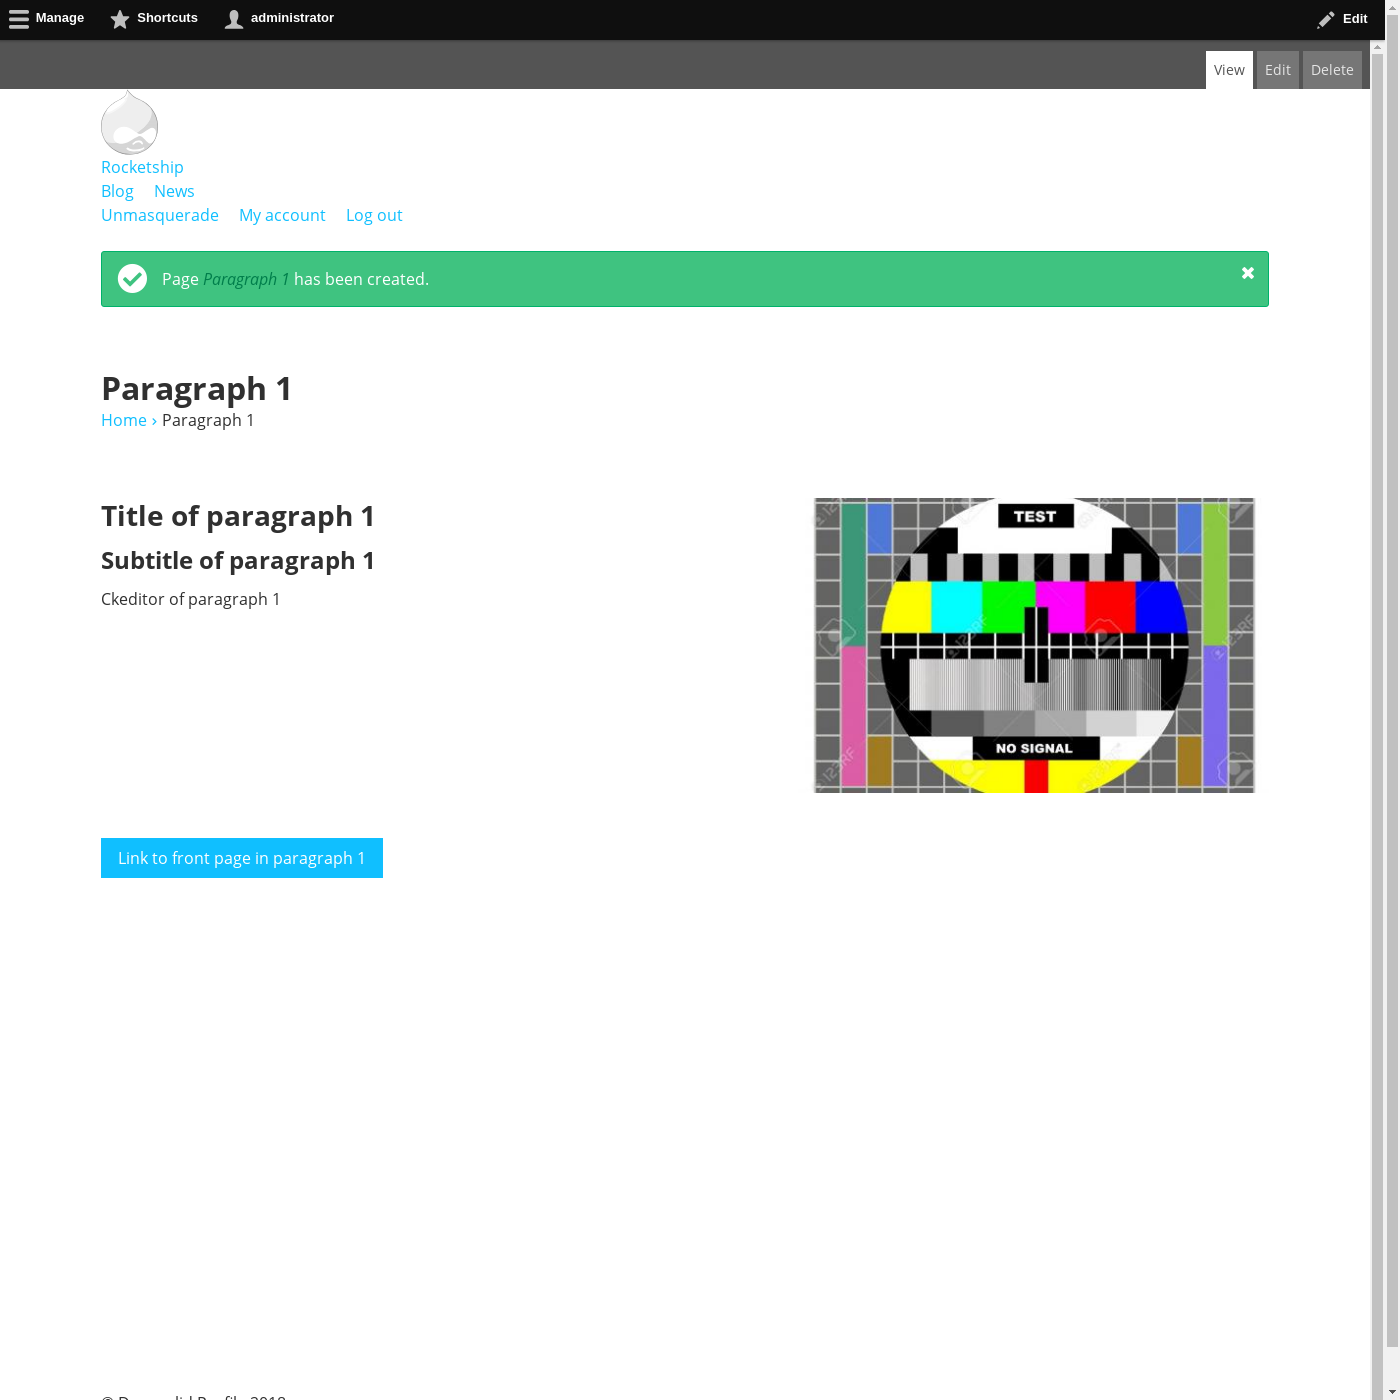
\includegraphics[width=1\textwidth]{img/p001.png}
\end{figure}

\clearpage
\paragraph{Paragraph 2: Image}
De tweede Paragraph is een blok die een afbeelding bevat en linkt naar een andere pagina.
\begin{figure}[h]
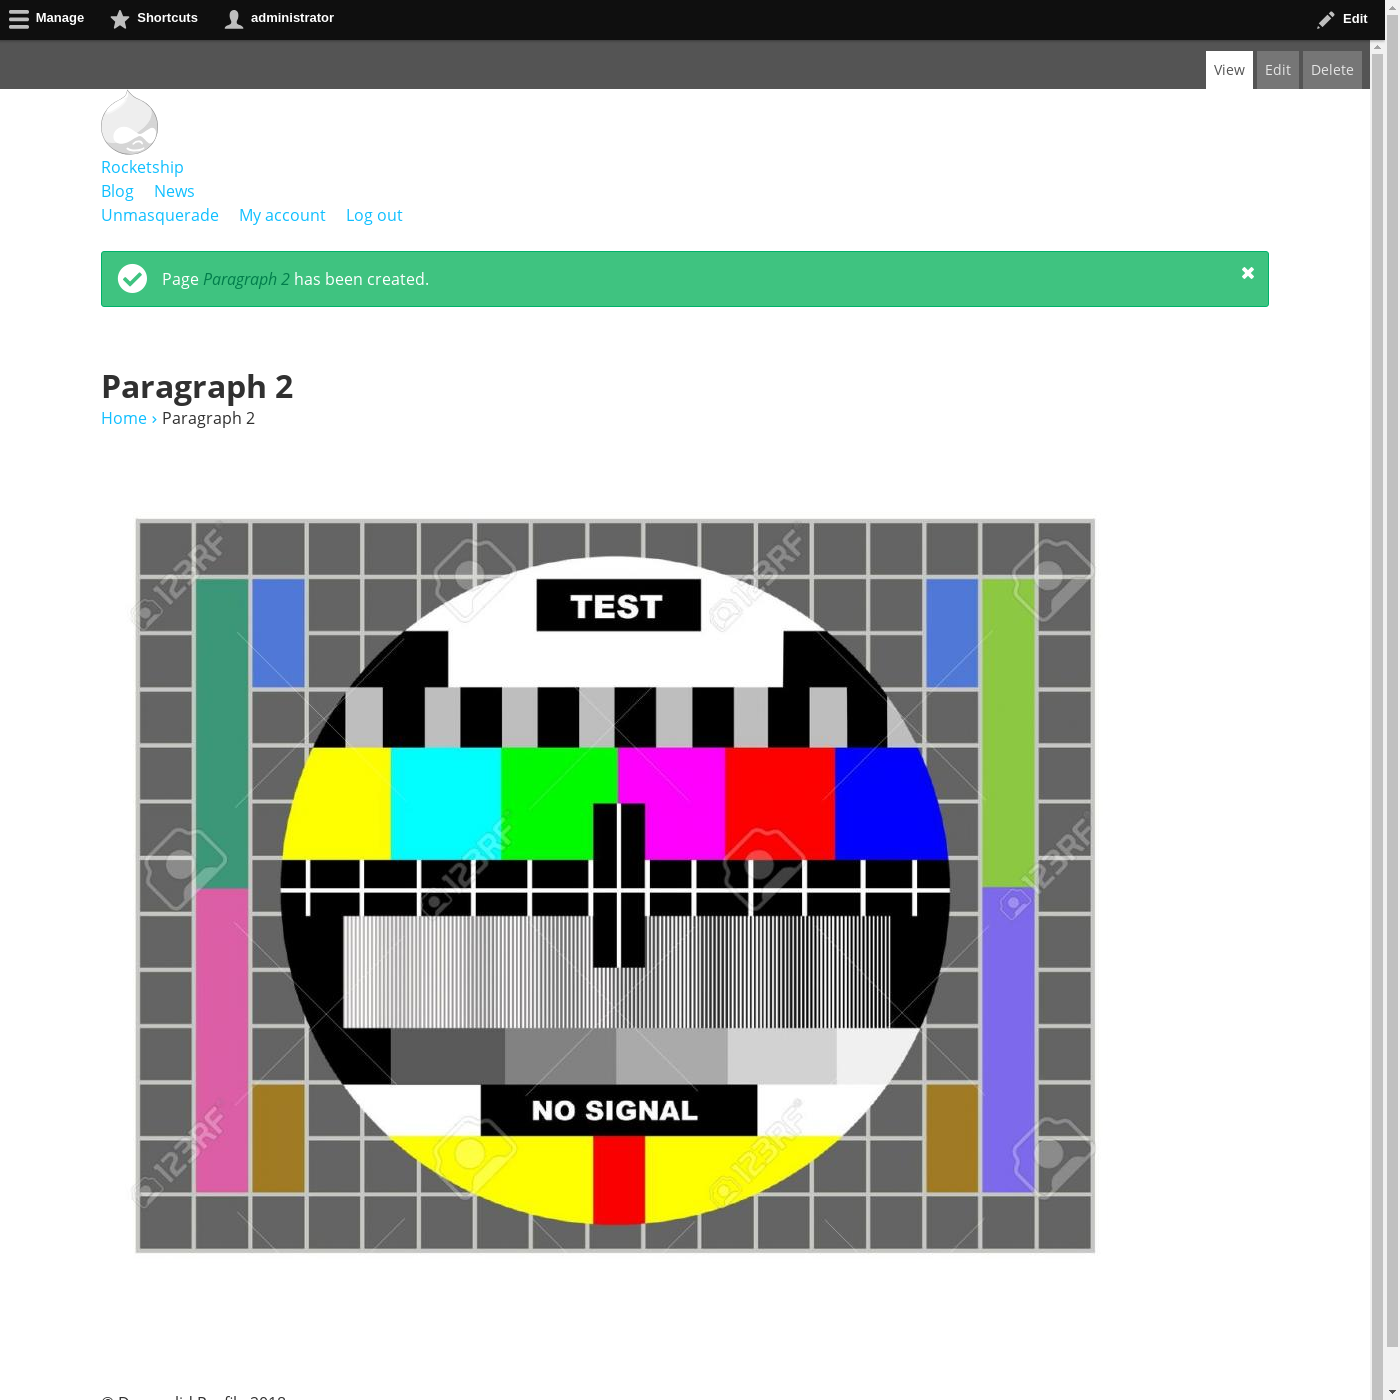
\includegraphics[width=1\textwidth]{img/p002.png}
\end{figure}

\clearpage
\paragraph{Paragraph 3: Text main}
De derde Paragraph is een blok met een titel, een teaser, een tekstveld en een button die linkt naar een andere pagina.
\begin{figure}[h]
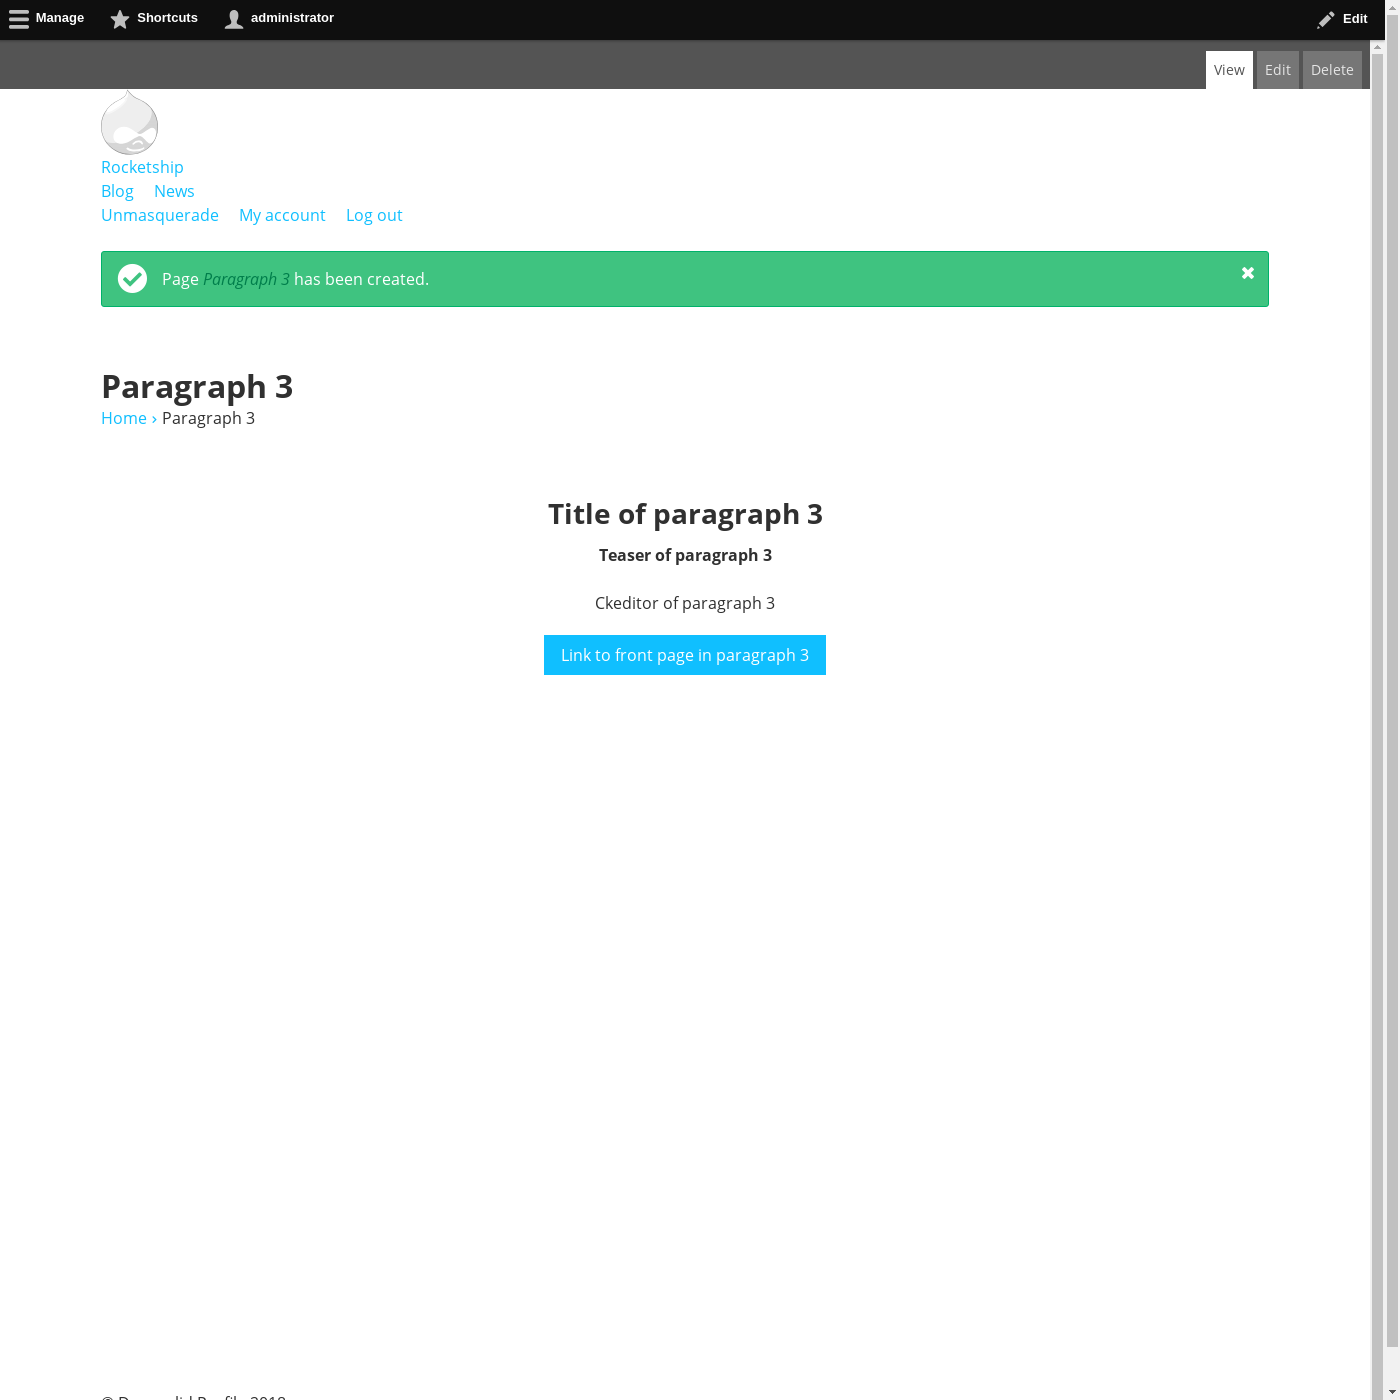
\includegraphics[width=1\textwidth]{img/p003.png}
\end{figure}

\clearpage
\paragraph{Paragraph 4: FAQ}
De vierde Paragraph is een blok met een titel, een subtitel en een teaser met daaronder veelgestgestelde vragen die kunnen open geklikt worden om het antwoord er op te zien.
\begin{figure}[h]
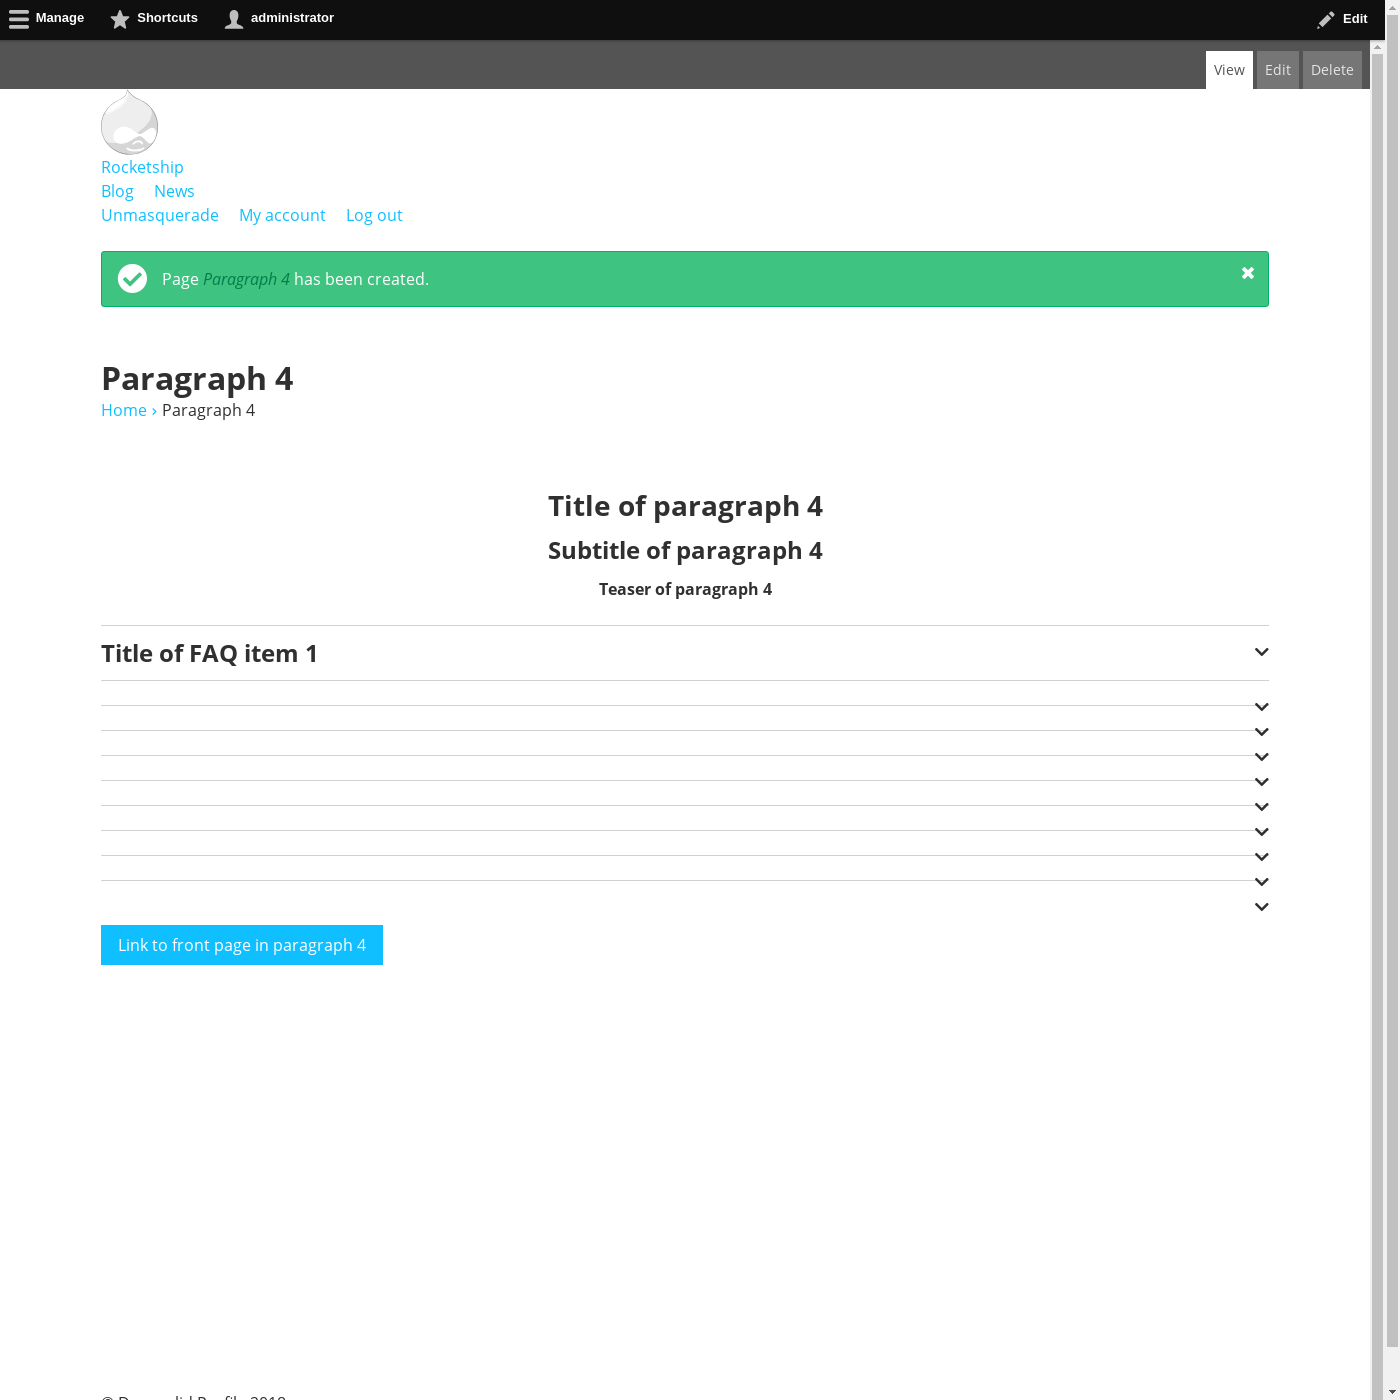
\includegraphics[width=1\textwidth]{img/p004.png}
\end{figure}

\clearpage
\paragraph{Paragraph 5: Testimonial}
De vijfde Paragraph is een blok die een afbeelding, een quote, een  naam, een extra tekstveld en een link naar een andere pagina bevat.
\begin{figure}[h]
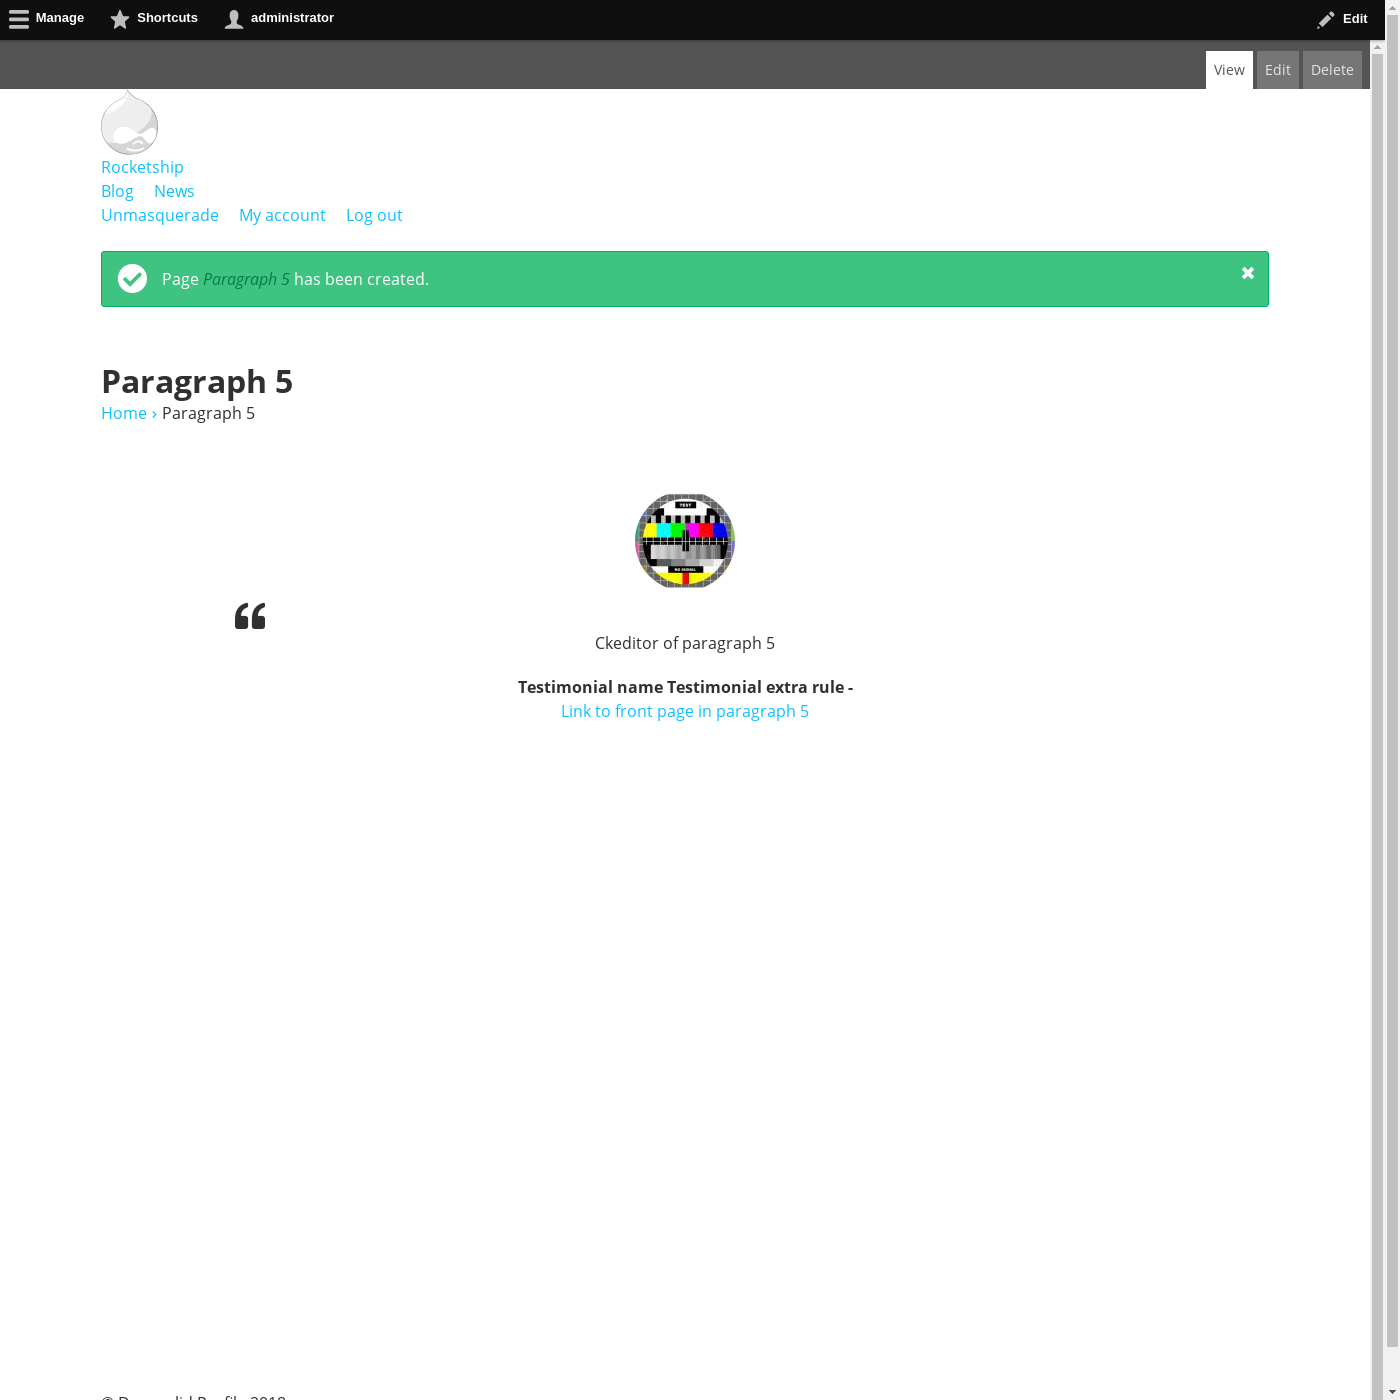
\includegraphics[width=1\textwidth]{img/p005.png}
\end{figure}

\clearpage
\paragraph{Paragraph 6: Video}
De zesde Paragraph is een blok die een youtube of vimeo video bevat.
\begin{figure}[h]
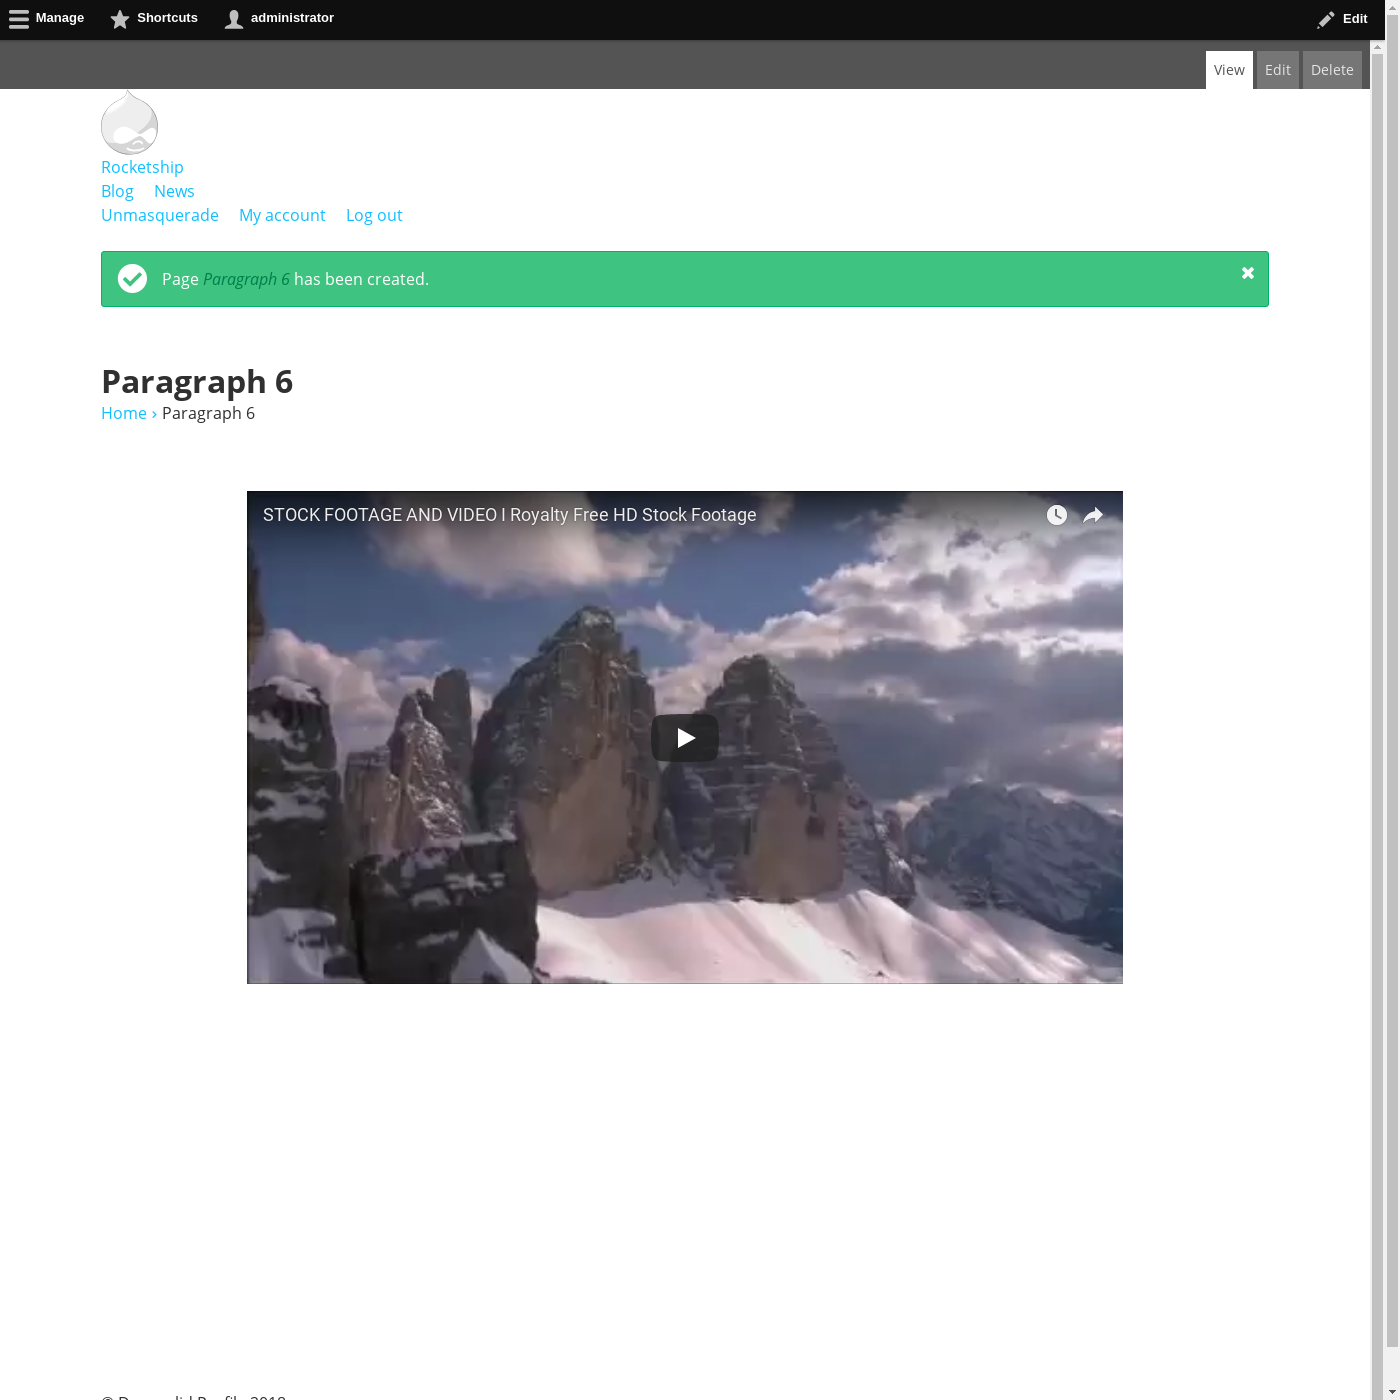
\includegraphics[width=1\textwidth]{img/p006.png}
\end{figure}

\clearpage
\paragraph{Paragraph 7: USP}
De zevende Paragraph is een blok met een titel, subtitel en teaser. Hieronder staat een USP item dat een afbeelding, titel en tekstveld bevat. Onder de USP items staat er ook nog eens een button die linkt naar een andere pagina.
\begin{figure}[h]
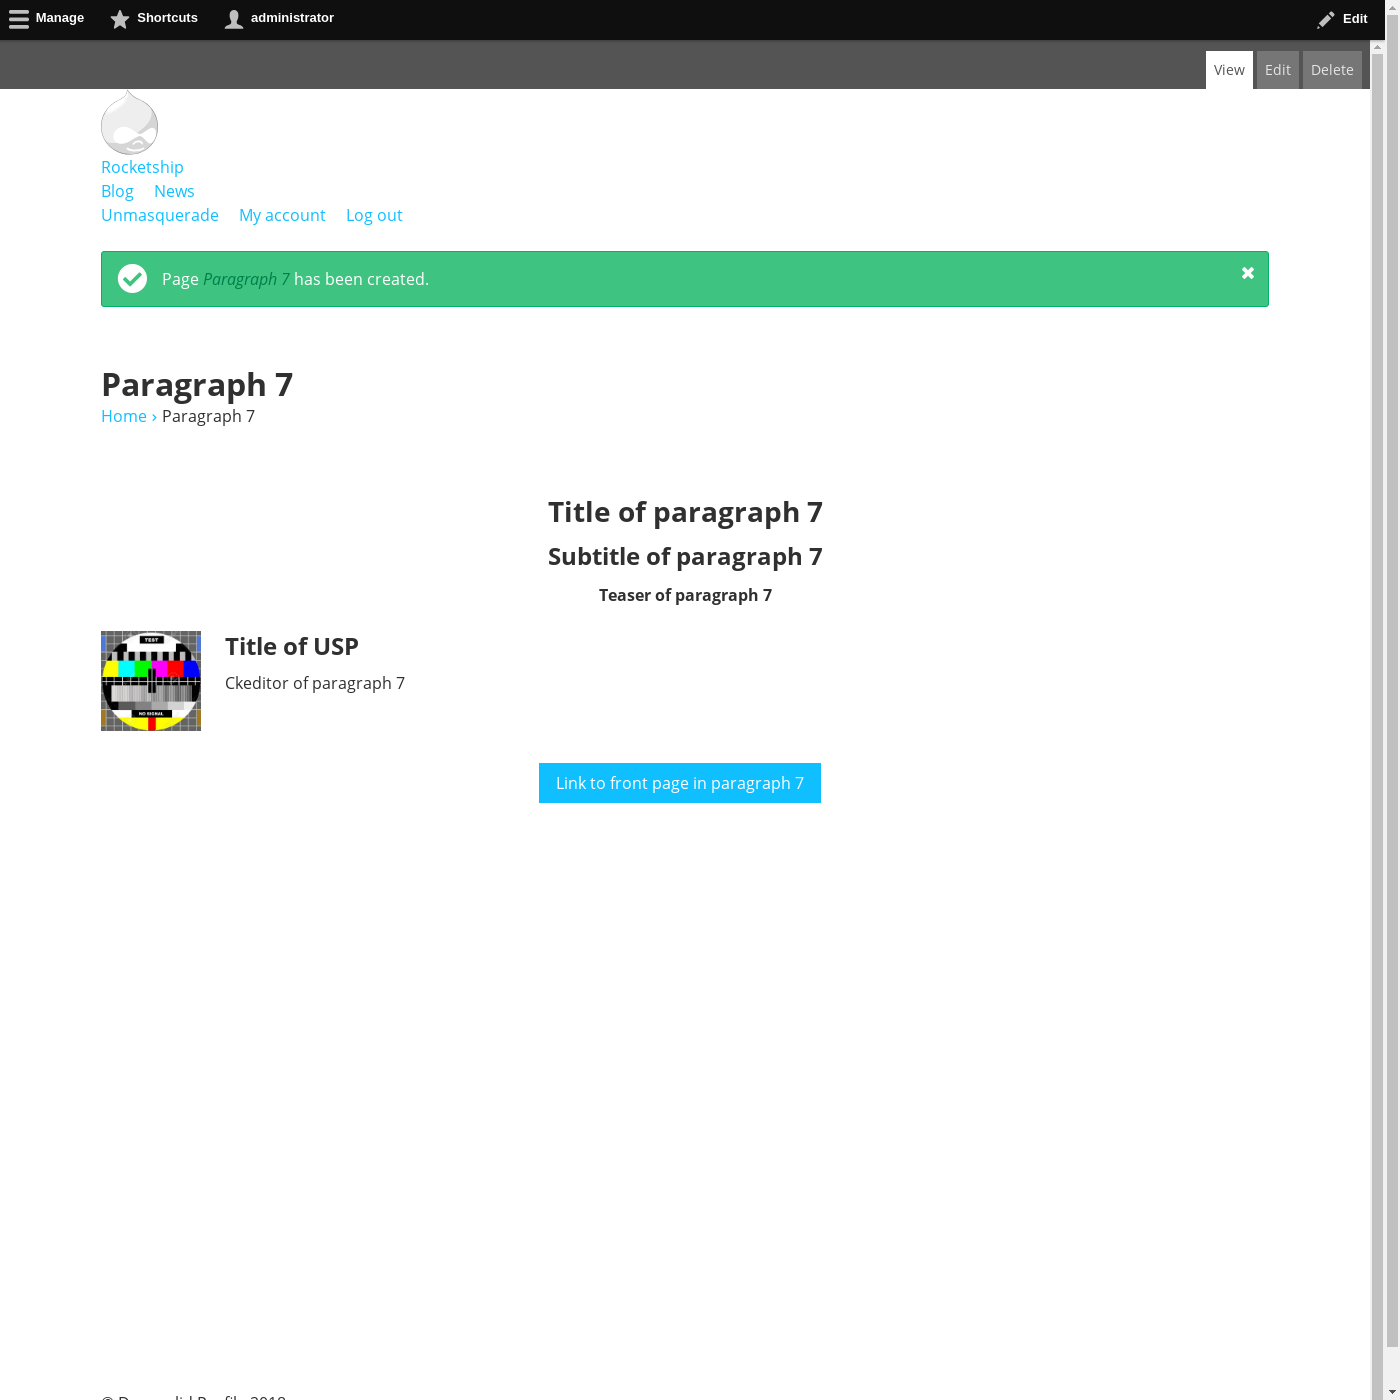
\includegraphics[width=1\textwidth]{img/p007.png}
\end{figure}

\clearpage
\paragraph{Paragraph 8: Focus}
De achtste Paragraph is gelijkaardig aan de derde Paragraph en is een blok met een titel, subtitel, teaser en button die linkt naar een andere pagina.
\begin{figure}[h]
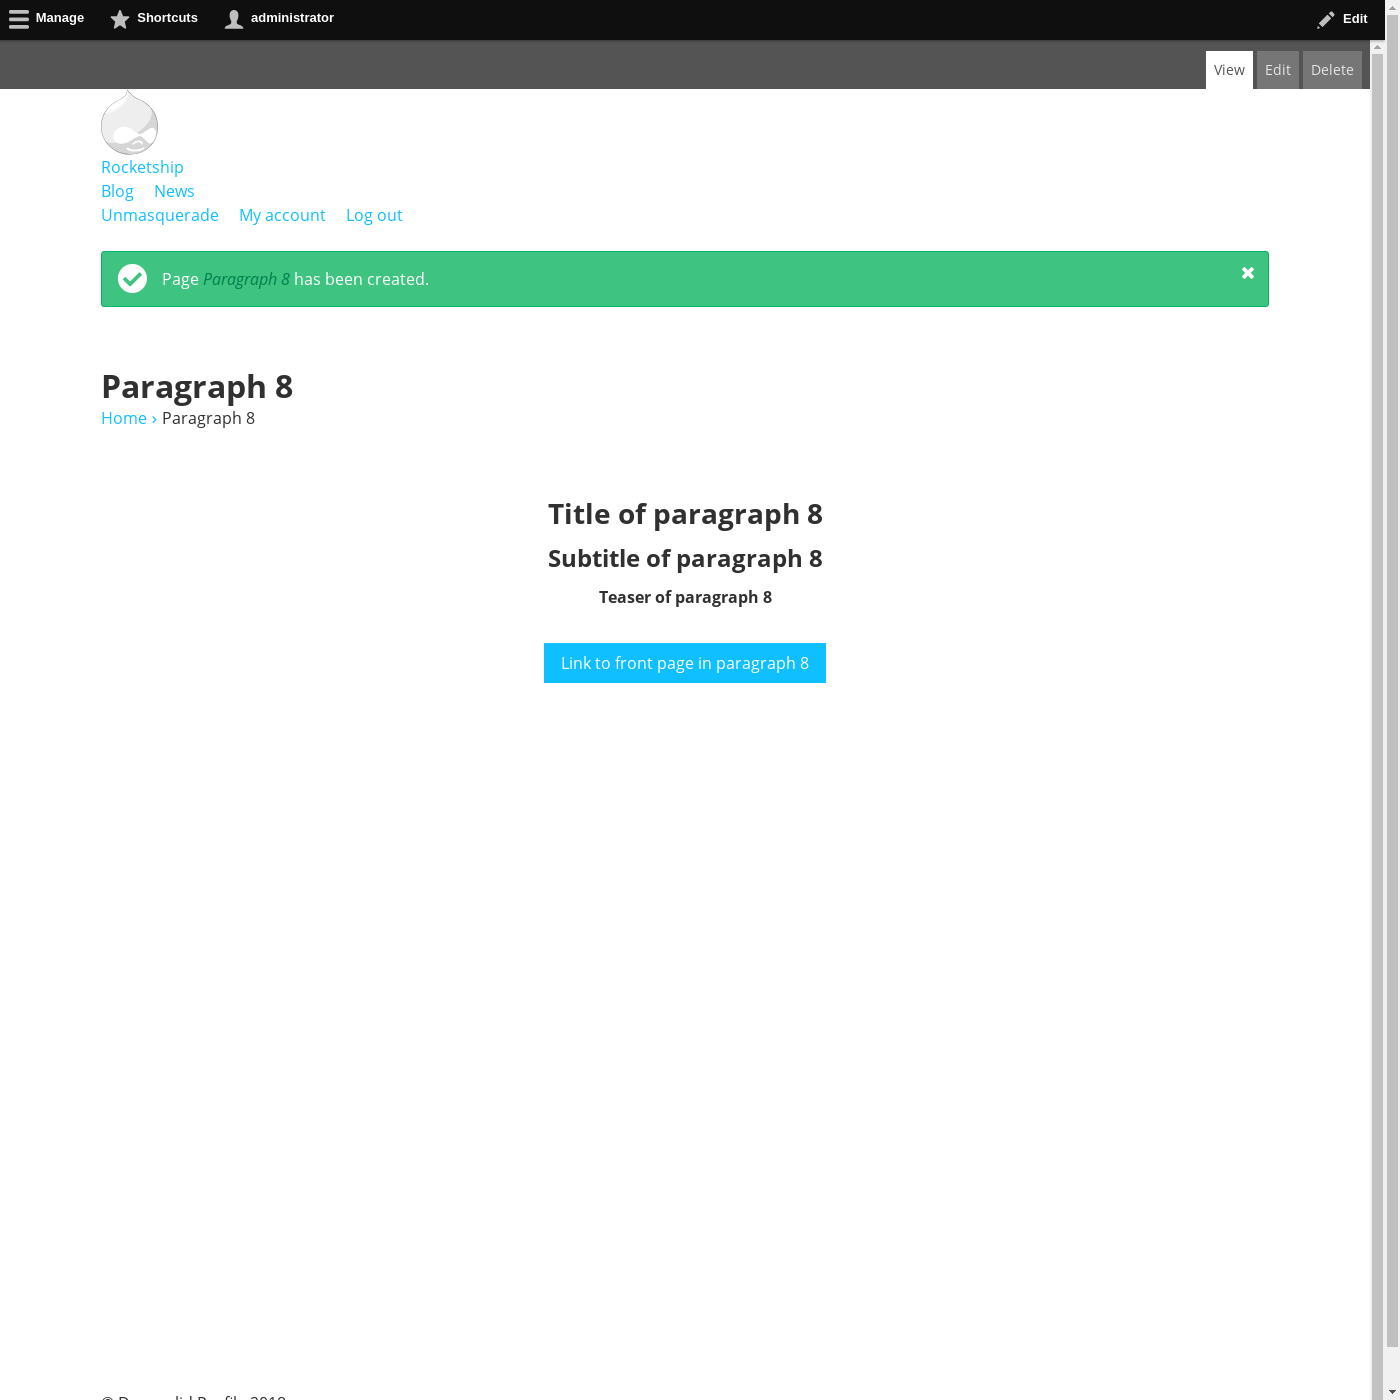
\includegraphics[width=1\textwidth]{img/p008.png}
\end{figure}

\clearpage
\paragraph{Paragraph 9: Photo gallery}
De negende Paragraph is een blok met een titel, subtitel en teaser. Hieronder staan afbeeldingen die linken naar een andere pagina en de blok wordt afgesloten met een button die ook een link bevat.
\begin{figure}[h]
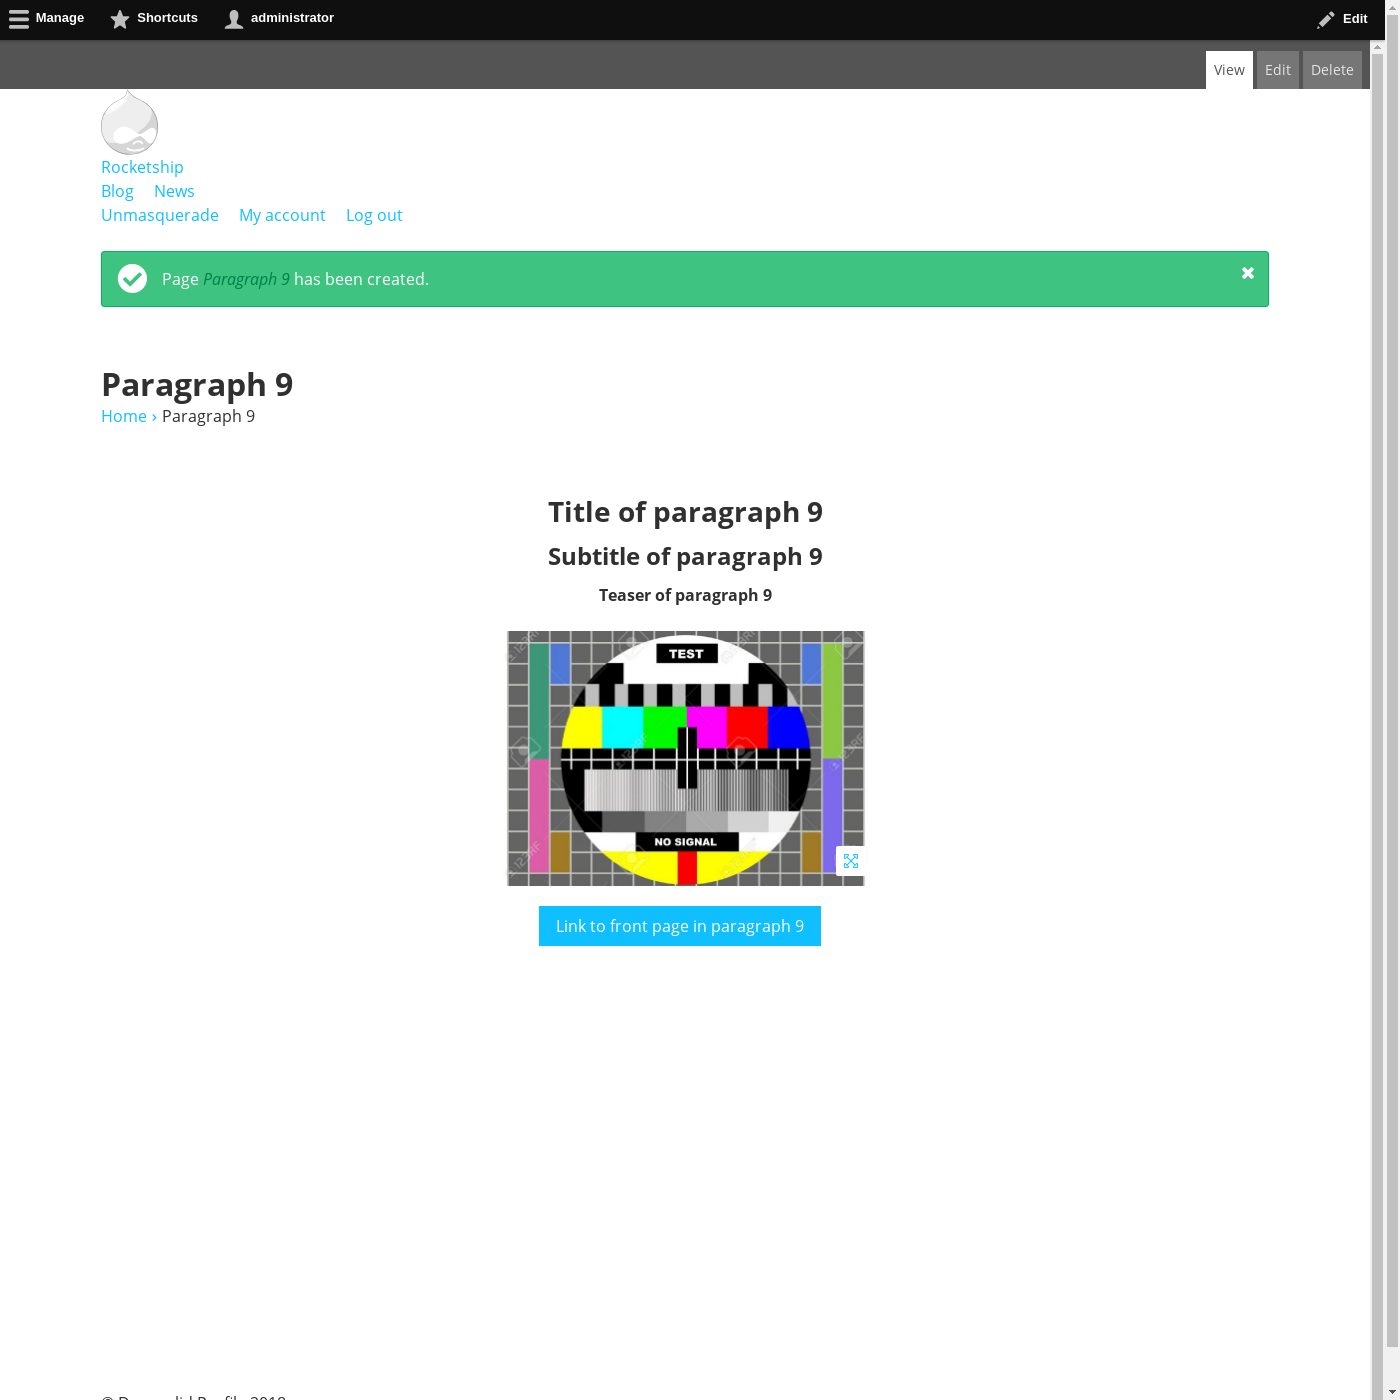
\includegraphics[width=1\textwidth]{img/p009.png}
\end{figure}

\clearpage
\paragraph{Paragraph 10: Logo bar}
De tiende Paragraph is een blok met een titel, subtitel, teaser, logo en button met een link.
\begin{figure}[h]
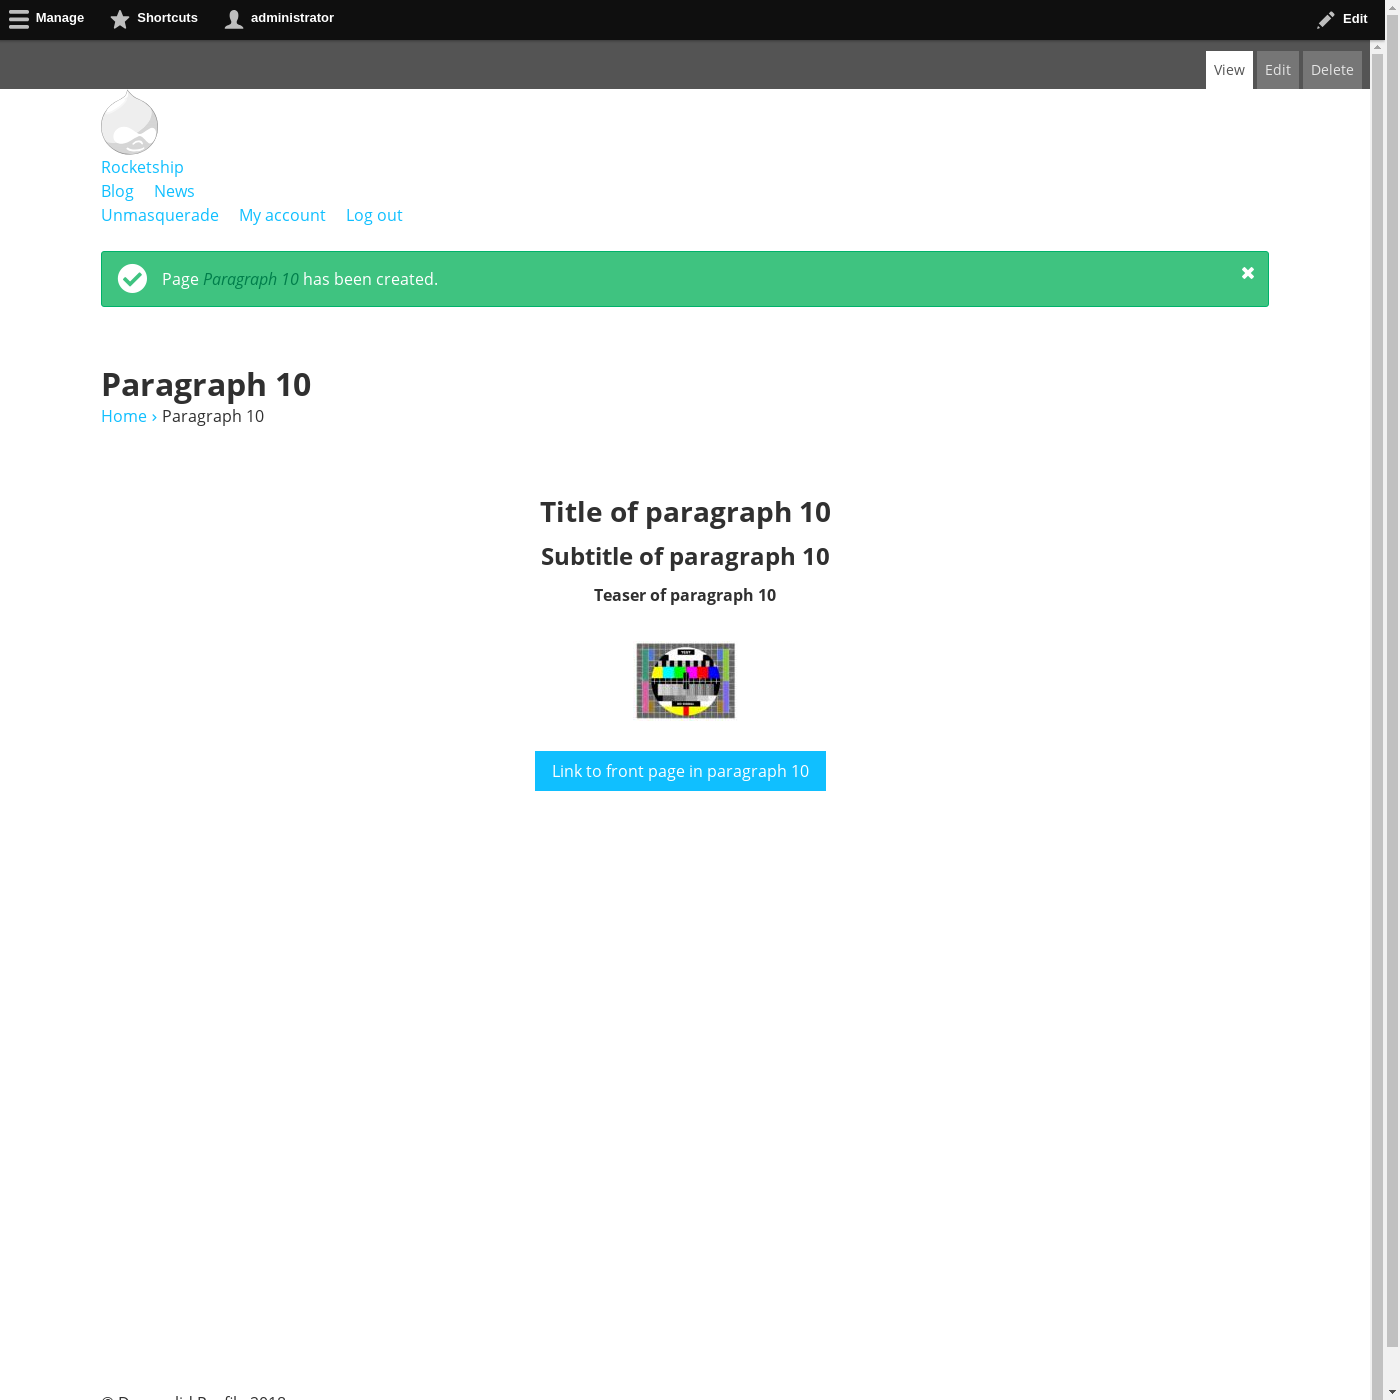
\includegraphics[width=1\textwidth]{img/p010.png}
\end{figure}

\clearpage
\paragraph{Paragraph 11: Form}
De elfde Paragraph is een blok met een formulier. Momenteel is het contact formulier het enige formulier dat met deze Paragraph kan aangemaakt worden.
\begin{figure}[h]
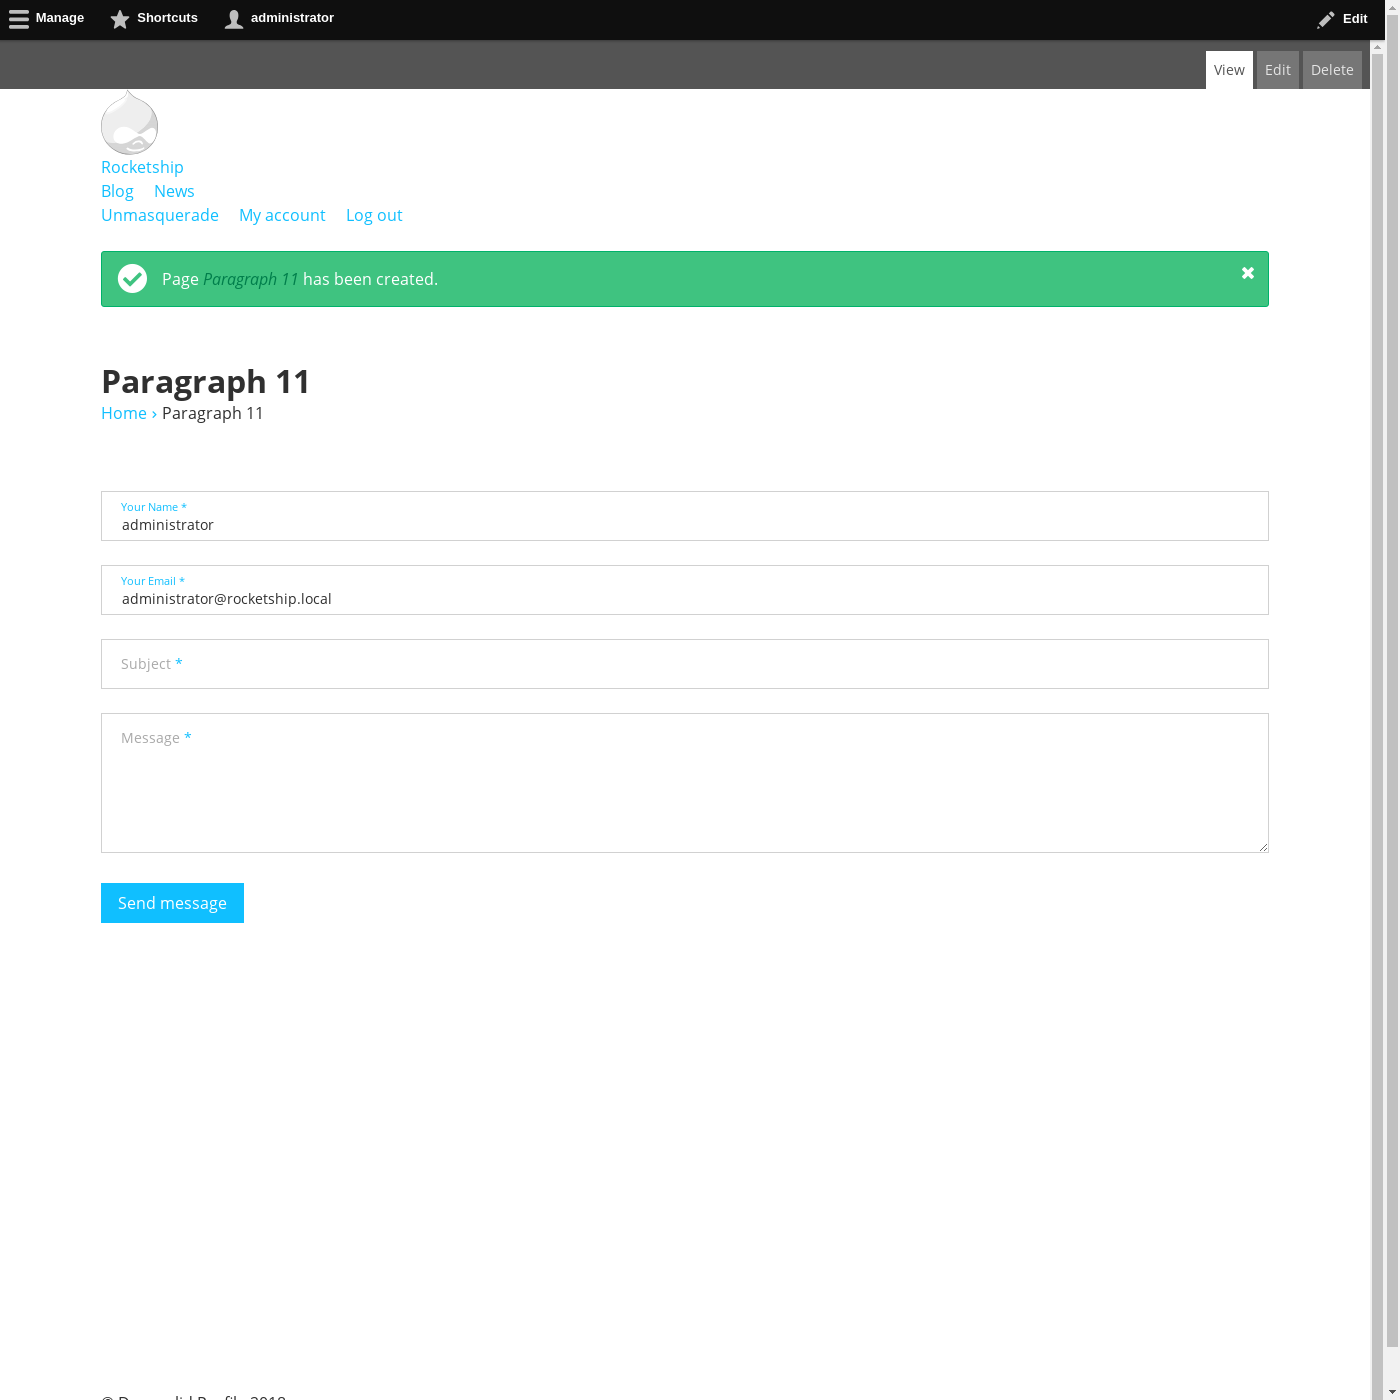
\includegraphics[width=1\textwidth]{img/p011.png}
\end{figure}


\clearpage
\paragraph{Paragraph 12: Guidance}
De twaalfde Paragraph is een blok die Guidance items bevat en deze items kunnen op verschillende manieren op de pagina geplaatsts worden, bijvoorbeeld per 2 of per 4 naast elkaar. Zo een Guidance item bevat een titel, een teaser en linkt naar een andere pagina. De blok wordt afgesloten met een button die een link bevat.
\begin{figure}[h]
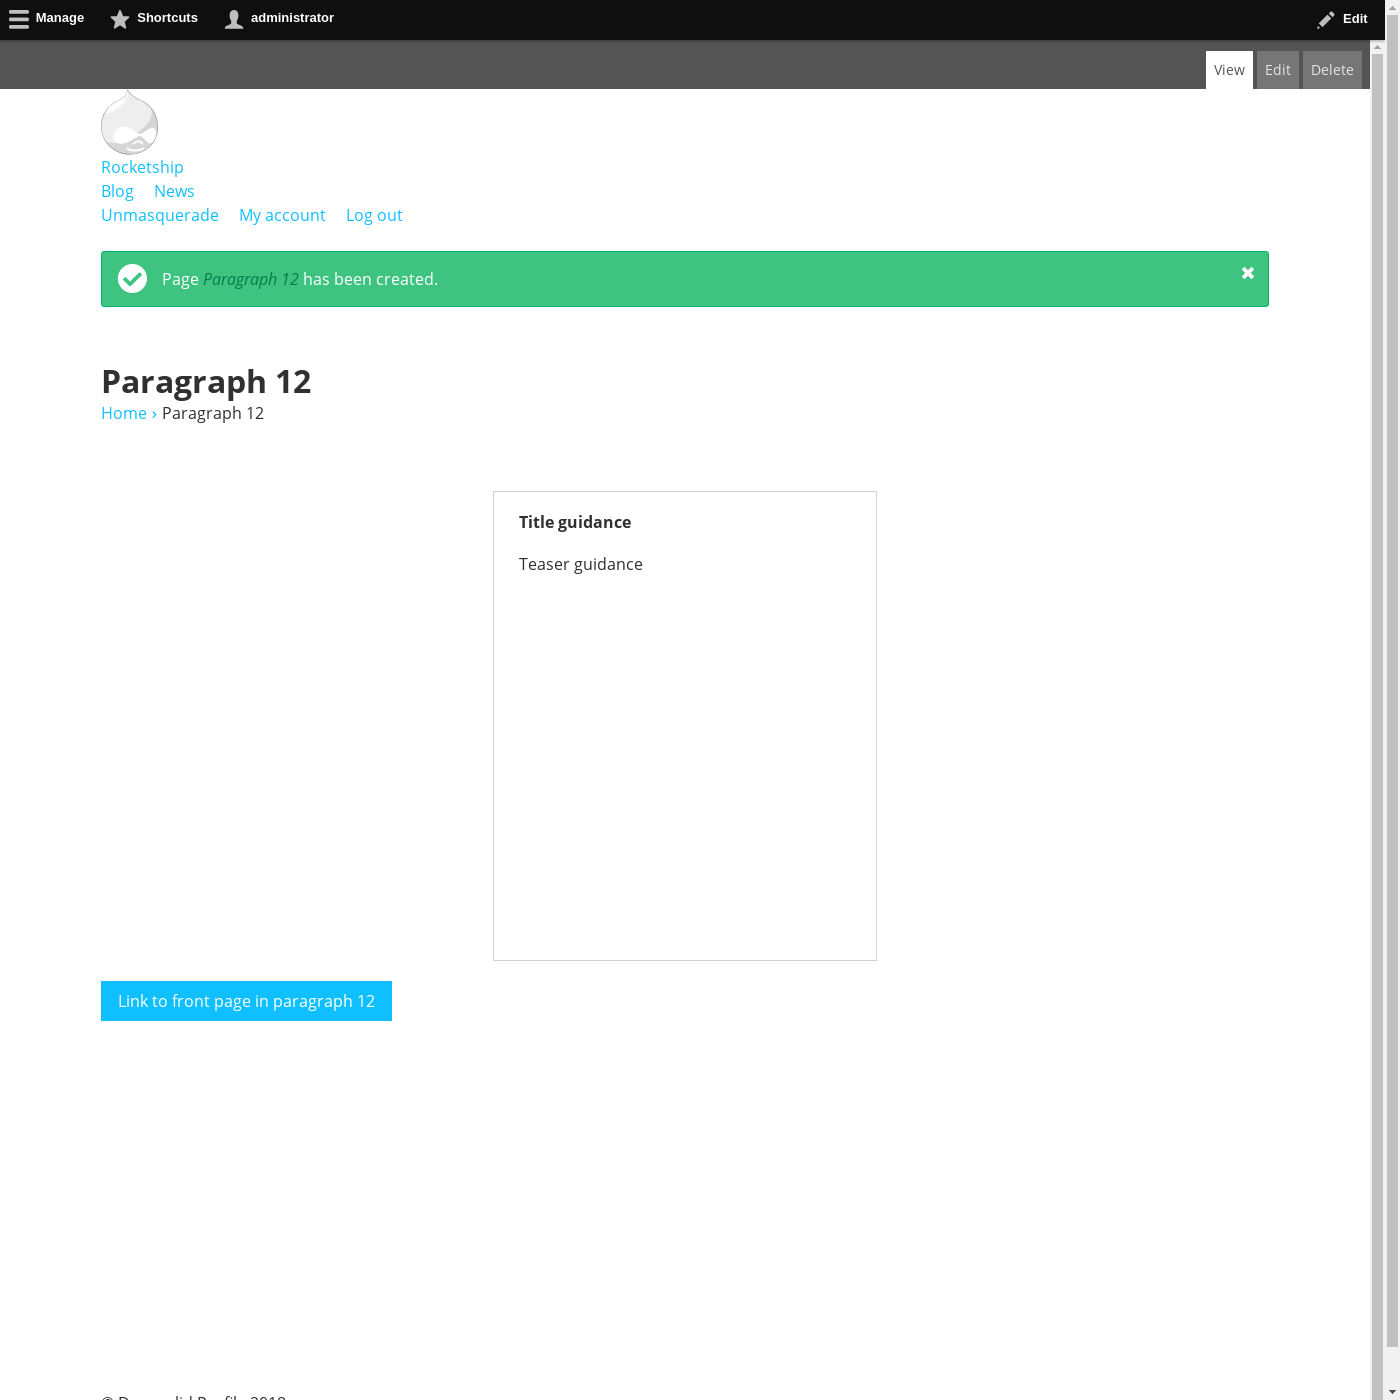
\includegraphics[width=1\textwidth]{img/p012.png}
\end{figure}

\clearpage
\section{Installatie en configuratie}
De installatie begon net zoals in het hoofdstuk methodologie met de lokale en globale installatie van Nightwatch met de respectievelijke commando's "npm install nightwatch" "npm install -g nightwatch".

Voor deze proof of concept wordt gebruik gemaakt van de \textcite{SeleniumStandaloneServer} om de mogelijkheden in verband met het parallel uitvoeren van testen en cross-browser testen aan te tonen. \textcite{ChromeDriver2018} en \textcite{GeckoDriver} worden gedownload met "npm install chromedriver geckodriver". Hiermee kunnen de testen uitgevoerd worden op Google Chrome en op Mozilla Firefox.

Er werden twee configuratiebestanden aangemaakt. Een globals.js bestand dat de globale variabelen bevat en een nightwatch.json bestand dat de hoofdconfiguratie bevat. Hierin staat de configuratie voor het parallel uitvoeren van testen, de configuratie om Selenium Standalone Server, ChromeDriver en GeckoDriver te gebruiken. Hierin staan ook vijf omgevingen gedefinïeerd. De eerste omgeving is de standaard Chrome omgeving. De tweede omgeving is de Chrome desktop omgeving die de testen uitvoert op de Chrome browser met een resolutie van 1366 pixels breed en 768 pixels hoog. De derde omgeving is de Chrome \gls{headless} omgeving. De vierde omgeving is de Firefox desktop omgeving die de testen uitvoert op de Firefox browser met een resolutie van 1366 pixels breed en 768 pixels hoog. De vijfde en laatste omgeving is de Firefox \gls{headless} omgeving.

\paragraph{globals.js}
\lstinputlisting[breaklines=true]{poc/globals.js}
\paragraph{nightwatch.json}
\lstinputlisting[breaklines=true]{poc/nightwatch.json}

\clearpage
\section{Testsuite}
Elke test start met het openen van een browser, te surfen naar de website en in te loggen als administrator. Dan wordt een pagina aangemaakt met de Paragraph die bij de test hoort en worden de velden van de Paragraph ingevuld. Ten slotte wordt elke test afgesloten met het uitloggen en sluiten van de browser.

\paragraph{Lijst van testen}
\begin{enumerate}
\item \hyperref[test1]{Test Paragraph 1}
\item \hyperref[test2]{Test Paragraph 2}
\item \hyperref[test3]{Test Paragraph 3}
\item \hyperref[test4]{Test Paragraph 4}
\item \hyperref[test5]{Test Paragraph 5}
\item \hyperref[test6]{Test Paragraph 6}
\item \hyperref[test7]{Test Paragraph 7}
\item \hyperref[test8]{Test Paragraph 8}
\item \hyperref[test9]{Test Paragraph 9}
\item \hyperref[test10]{Test Paragraph 10}
\item \hyperref[test11]{Test Paragraph 11}
\item \hyperref[test12]{Test Paragraph 12}
\end{enumerate}

\paragraph{Uitvoeringstijd testsuite}
\begin{tabular}{ |c| c| }
\hline
	Google Chrome standaard & 1 minuut 44 seconden \\
\hline
	Google Chrome desktop & 1 minuut 59 seconden \\
\hline
 	Google Chrome headless & 1 minuut 19 seconden \\
\hline
 	Mozilla Firefox desktop & 2 minuten 10 seconden \\
\hline
 	Mozilla Firefox headless & 1 minuut 36 seconden \\
\hline
\end{tabular}


\clearpage
\paragraph{Test Paragraph 1}
\label{test1}
Opbouw test: 
\begin{itemize}
\item test opstarten zoals in het begin van dit deel toegelicht
\item titel en subtitel invullen
\item tekstveld invullen
\item afbeelding met alt tekst toevoegen
\item de viewmode selecteren, in deze test image\_right
\item button met link en link tekst toevoegen
\item pagina opslaan en aanmaken
\item screenshot nemen van de aangemaakte pagina
\item controleren dat de titel en subtitel correct zijn
\item controleren dat het tekstveld correct is
\item controleren dat de alt tekst van de afbeelding correct is
\item controleren dat de correcte view mode is gebruikt
\item controleren dat de button correct is aangemaakt
\item test afsluiten zoals in het begin van dit deel toegelicht
\end{itemize}
\paragraph{testParagraph001.js}
\lstinputlisting[breaklines=true]{poc/testParagraph001.js}

\clearpage
\paragraph{Test Paragraph 2}
\label{test2}
Opbouw test: 
\begin{itemize}
\item test opstarten zoals in het begin van dit deel toegelicht
\item afbeelding met alt tekst toevoegen
\item link toevoegen aan de afbeelding
\item pagina opslaan en aanmaken
\item screenshot nemen van de aangemaakte pagina
\item controleren dat de alt tekst van de afbeelding correct is
\item controleren dat de link op de afbeelding werkt
\item test afsluiten zoals in het begin van dit deel toegelicht
\end{itemize}
\paragraph{testParagraph002.js}
\lstinputlisting[breaklines=true]{poc/testParagraph002.js}

\clearpage
\paragraph{Test Paragraph 3}
\label{test3}
Opbouw test: 
\begin{itemize}
\item test opstarten zoals in het begin van dit deel toegelicht
\item titel en teaser invullen
\item tekstveld invullen
\item de viewmode selecteren, in deze test centered
\item button met link en link tekst toevoegen
\item pagina opslaan en aanmaken
\item screenshot nemen van de aangemaakte pagina
\item controleren dat de titel en teaser correct zijn
\item controleren dat het tekstveld correct is
\item controleren dat de correcte view mode is gebruikt
\item controleren dat de button correct is aangemaakt
\item test afsluiten zoals in het begin van dit deel besproken
\end{itemize}
\paragraph{testParagraph003.js}
\lstinputlisting[breaklines=true]{poc/testParagraph003.js}

\clearpage
\paragraph{Test Paragraph 4}
\label{test4}
Opbouw test: 
\begin{itemize}
\item test opstarten zoals in het begin van dit deel toegelicht
\item titel, subtitel en teaser invullen
\item titel  en tekstveld van een FAQ item invullen
\item button met link en link tekst toevoegen
\item pagina opslaan en aanmaken
\item screenshot nemen van de aangemaakte pagina
\item controleren dat de titel, subtitel en teaser correct zijn
\item controleren dat het FAQ item correct is aangemaakt
\item controleren dat de button correct is aangemaakt
\item test afsluiten zoals in het begin van dit deel besproken
\end{itemize}
\paragraph{testParagraph004.js}
\lstinputlisting[breaklines=true]{poc/testParagraph004.js}

\clearpage
\paragraph{Test Paragraph 5}
\label{test5}
Opbouw test: 
\begin{itemize}
\item test opstarten zoals in het begin van dit deel toegelicht
\item afbeelding met alt tekst toevoegen
\item tekstveld invullen
\item Testimonial naam en extra regel invullen
\item Link aan testimonial toevoegen
\item pagina opslaan en aanmaken
\item screenshot nemen van de aangemaakte pagina
\item controleren dat het tekstveld correct is
\item controleren dat de naam en extra regel van het Testimonial item correct zijn
\item controleren dat de alt tekst van de afbeelding correct is
\item controleren dat de correcte view mode is gebruikt
\item controleren dat de Testimonial link correct werkt
\item test afsluiten zoals in het begin van dit deel toegelicht
\end{itemize}
\paragraph{testParagraph005.js}
\lstinputlisting[breaklines=true]{poc/testParagraph005.js}

\clearpage
\paragraph{Test Paragraph 6}
\label{test6}
Opbouw test: 
\begin{itemize}
\item test opstarten zoals in het begin van dit deel toegelicht
\item video link toevoegen
\item pagina opslaan en aanmaken
\item screenshot nemen van de aangemaakte pagina
\item controleren de video is correct is toegevoegd
\item test afsluiten zoals in het begin van dit deel toegelicht
\end{itemize}
\paragraph{testParagraph006.js}
\lstinputlisting[breaklines=true]{poc/testParagraph006.js}

\clearpage
\paragraph{Test Paragraph 7}
\label{test7}
Opbouw test: 
\begin{itemize}
\item test opstarten zoals in het begin van dit deel toegelicht
\item titel, subtitel en teaser invullen
\item titel van het USP item invullen
\item afbeelding met alt tekst toevoegen aan het USP item
\item tekstveld van het USP item invullen
\item link aan het USP item toevoegen
\item button met link en link tekst toevoegen
\item pagina opslaan en aanmaken
\item screenshot nemen van de aangemaakte pagina
\item controleren dat de titel, subtitel en teaser correct zijn
\item controleren dat de titel en tekstveld van het USP item correct zijn
\item controleren dat de alt tekst van de afbeelding van het USP item correct is
\item controleren dat de link van het USP item correct werkt
\item controleren dat de button correct is aangemaakt
\item test afsluiten zoals in het begin van dit deel toegelicht
\end{itemize}
\paragraph{testParagraph007.js}
\lstinputlisting[breaklines=true]{poc/testParagraph007.js}

\clearpage
\paragraph{Test Paragraph 8}
\label{test8}
Opbouw test: 
\begin{itemize}
\item test opstarten zoals in het begin van dit deel toegelicht
\item titel, subtitel en teaser invullen
\item button met link en link tekst toevoegen
\item pagina opslaan en aanmaken
\item screenshot nemen van de aangemaakte pagina
\item controleren dat de titel, subtitel en teaser correct zijn
\item controleren dat de button correct is aangemaakt
\item test afsluiten zoals in het begin van dit deel toegelicht
\end{itemize}
\paragraph{testParagraph008.js}
\lstinputlisting[breaklines=true]{poc/testParagraph008.js}

\clearpage
\paragraph{Test Paragraph 9}
\label{test9}
Opbouw test: 
\begin{itemize}
\item test opstarten zoals in het begin van dit deel toegelicht
\item titel, subtitel en teaser invullen
\item afbeelding met alt tekst toevoegen
\item button met link en link tekst toevoegen
\item pagina opslaan en aanmaken
\item screenshot nemen van de aangemaakte pagina
\item controleren dat de titel, subtitel en teaser correct zijn
\item controleren dat de alt tekst van de afbeelding correct is
\item controleren dat de button correct is aangemaakt
\item test afsluiten zoals in het begin van dit deel toegelicht
\end{itemize}
\paragraph{testParagraph009.js}
\lstinputlisting[breaklines=true]{poc/testParagraph009.js}

\clearpage
\paragraph{Test Paragraph 10}
\label{test10}
Opbouw test: 
\begin{itemize}
\item test opstarten zoals in het begin van dit deel toegelicht
\item titel, subtitel en teaser invullen
\item logo met alt tekst toevoegen
\item link aan het logo toevoegen
\item button met link en link tekst toevoegen
\item pagina opslaan en aanmaken
\item screenshot nemen van de aangemaakte pagina
\item controleren dat de titel, subtitel en teaser correct zijn
\item controleren dat de alt tekst van het logo correct is
\item controleren dat de link van het logo correct werkt
\item controleren dat de button correct is aangemaakt
\item test afsluiten zoals in het begin van dit deel toegelicht
\end{itemize}
\paragraph{testParagraph010.js}
\lstinputlisting[breaklines=true]{poc/testParagraph010.js}

\clearpage
\paragraph{Test Paragraph 11}
\label{test11}
Opbouw test: 
\begin{itemize}
\item test opstarten zoals in het begin van dit deel toegelicht
\item contact formulier selecteren
\item pagina opslaan en aanmaken
\item screenshot nemen van de aangemaakte pagina
\item controleren dat het contact formulier correct is aangemaakt en werkt
\item test afsluiten zoals in het begin van dit deel toegelicht
\end{itemize}
\paragraph{testParagraph011.js}
\lstinputlisting[breaklines=true]{poc/testParagraph011.js}

\clearpage
\paragraph{Test Paragraph 12}
\label{test12}
Opbouw test: 
\begin{itemize}
\item test opstarten zoals in het begin van dit deel toegelicht
\item de viewmode selecteren, hier default\_large
\item titel en teaser van Guidance item invullen
\item afbeelding met alt tekst toevoegen aan het Guidance item
\item link aan het Guidance item toevoegen
\item button met link en link tekst toevoegen
\item pagina opslaan en aanmaken
\item screenshot nemen van de aangemaakte pagina
\item controleren dat de titel en teaser van het Guidance item correct zijn
\item controleren dat de link van het Guidance item correct werkt
\item controleren dat de button correct is aangemaakt
\item test afsluiten zoals in het begin van dit deel toegelicht
\end{itemize}
\paragraph{testParagraph012.js}
\lstinputlisting[breaklines=true]{poc/testParagraph012.js}

\clearpage
\section{Commando's}
Voor de testen zo leesbaar en gebruiksvriendelijk mogelijk te maken werden er commando's geschreven die de achterliggende code weg abstraheren.

\paragraph{Lijst van commando's}
\begin{enumerate}
\item \hyperref[commando1]{drupalAssertParagraphButton}
\item \hyperref[commando2]{drupalAssertParagraphCkeditor}
\item \hyperref[commando3]{drupalAssertParagraphFaq}
\item \hyperref[commando4]{drupalAssertParagraphForm}
\item \hyperref[commando5]{drupalAssertParagraphGuidance}
\item \hyperref[commando6]{drupalAssertParagraphImage}
\item \hyperref[commando7]{drupalAssertParagraphLink}
\item \hyperref[commando8]{drupalAssertParagraphTestimonial}
\item \hyperref[commando9]{drupalAssertParagraphTitle}
\item \hyperref[commando10]{drupalAssertParagraphUsp}
\item \hyperref[commando11]{drupalAssertParagraphVideo}
\item \hyperref[commando12]{drupalAssertParagraphViewmode}
\item \hyperref[commando13]{drupalCreatePageWithParagraph}
\item \hyperref[commando14]{drupalDeletePage}
\item \hyperref[commando15]{drupalInputParagraphButton}
\item \hyperref[commando16]{drupalInputParagraphCkeditor}
\item \hyperref[commando17]{drupalInputParagraphFaq}
\item \hyperref[commando18]{drupalInputParagraphForm}
\item \hyperref[commando19]{drupalInputParagraphGuidance}
\item \hyperref[commando20]{drupalInputParagraphImage}
\item \hyperref[commando21]{drupalInputParagraphLink}
\item \hyperref[commando22]{drupalInputParagraphTestimonial}
\item \hyperref[commando23]{drupalInputParagraphTitle}
\item \hyperref[commando24]{drupalInputParagraphUsp}
\item \hyperref[commando25]{drupalInputParagraphVideo}
\item \hyperref[commando26]{drupalInputParagraphViewmode}
\item \hyperref[commando27]{drupalLogin}
\item \hyperref[commando28]{drupalLoginAsAdmin}
\item \hyperref[commando29]{drupalLogout}
\item \hyperref[commando30]{drupalRelativeURL}
\item \hyperref[commando31]{drupalScreenshot}
\item \hyperref[commando32]{drupalSubmit}
\item \hyperref[commando33]{drupalUserIsLoggedIn}
\end{enumerate}

\clearpage
\paragraph{drupalAssertParagraphButton}
\label{commando1}
Dit commando gaat na of een button op een Paragraph correct is aangemaakt door de titel te vergelijken met de waarde meegegeven en door op de button te klikken en de url van de bezochte pagina te vergelijken met de meegegeven waarde.
\paragraph{drupalAssertParagraphButton.js}
\begin{lstlisting}[breaklines=true]
exports.command = function drupalAssertParagraphButton({ title, url }) {
  if (typeof title !== 'undefined') {
    this.assert.containsText('.paragraph .field--name-field-p-button a', title);
  }

  if (typeof url !== 'undefined') {
    this.waitForElementVisible('.paragraph .field--name-field-p-button a', this.globals.timeoutTime)
      .click('.paragraph .field--name-field-p-button a')
      .assert.urlEquals(url)
      .back();
  }

  return this;
};
\end{lstlisting}


\clearpage
\paragraph{drupalAssertParagraphCkeditor}
\label{commando2}
Dit commando gaat na of het tekstveld op een Paragraph correct is aangemaakt door het te vergelijken met de meegegeven waarde.
\paragraph{drupalAssertParagraphCkeditor.js}
\begin{lstlisting}[breaklines=true]
exports.command = function drupalAssertParagraphCkeditor({ text }) {
  if (typeof text !== 'undefined') {
    this.assert.containsText('.paragraph .field--name-field-p-text p', text);
  }

  return this;
};
\end{lstlisting}


\clearpage
\paragraph{drupalAssertParagraphFaq}
\label{commando3}
Dit commando gaat na of de FAQ Paragraph correct is aangemaakt door de titel en het tekstveld te vergelijken met de meegegeven waarden.
\paragraph{drupalAssertParagraphFaq.js}
\begin{lstlisting}[breaklines=true]
exports.command = function drupalAssertParagraphFaq({ title, ckeditor }) {
  if (typeof title !== 'undefined') {
    this.assert.containsText('.paragraph--type-p-004 .field__item--name-field-p-004-item:first-of-type h3', title);
  }

  if (typeof ckeditor !== 'undefined') {
    this.waitForElementVisible('.paragraph--type-p-004 .field__item--name-field-p-004-item:first-of-type h3', this.globals.timeoutTime)
      .click('.paragraph--type-p-004 .field__item--name-field-p-004-item:first-of-type h3')
      .assert.containsText('.paragraph--type-p-004 .field__item--name-field-p-004-item:first-of-type .tab-item__content', ckeditor);
  }

  return this;
};
\end{lstlisting}


\clearpage
\paragraph{drupalAssertParagraphForm}
\label{commando4}
Dit commando gaat na of de Paragraph met een contact formulier correct is aangemaakt.
\paragraph{drupalAssertParagraphForm.js}
\begin{lstlisting}[breaklines=true]
exports.command = function drupalAssertParagraphForm({ subject, message }) {
  this.waitForElementVisible('input[name="name"]', this.globals.timeoutTime)
    .assert.attributeEquals('input[name="name"]', 'value', this.globals.adminUsername)
    .assert.attributeEquals('input[name="email"]', 'value', this.globals.adminUsername + '@rocketship.local');

  if (typeof subject !== 'undefined') {
    this.setValue('input[name="subject"]', subject);
  }

  if (typeof message !== 'undefined') {
    this.setValue('textarea[name="message"]', message);
  }

  if (typeof subject !== 'undefined' && typeof message !== 'undefined') {
    this.click('#edit-actions-submit')
      .assert.urlEquals(this.globals.launch_url + '/')
      .back();
  }
  return this;
};
\end{lstlisting}


\clearpage
\paragraph{drupalAssertParagraphGuidance}
\label{commando5}
Dit commando gaat na of de Paragraph Guidance titel en teaser correct zijn aangemaakt door deze te vergelijken met de meegegeven waarde.
\paragraph{drupalAssertParagraphGuidance.js}
\begin{lstlisting}[breaklines=true]
exports.command = function drupalAssertParagraphGuidance({ title, teaser }) {
  if (typeof title !== 'undefined') {
    this.assert.containsText('.paragraph--type-p-012 .paragraph--type-p-012-child .field--name-field-p-title h4', title);
  }

  if (typeof teaser !== 'undefined') {
    this.assert.containsText('.paragraph--type-p-012 .paragraph--type-p-012-child .field--name-field-p-teaser', teaser);
  }

  return this;
};
\end{lstlisting}


\clearpage
\paragraph{drupalAssertParagraphImage}
\label{commando6}
Dit commando gaat na of een Paragraph afbeelding correct is aangemaakt door de alt tag te vergelijken met de meegegeven waarde. Voor de afbeeldingen van Paragraph 7 en 9 moet een ander argument meegegeven worden.
\paragraph{drupalAssertParagraphImage.js}
\begin{lstlisting}[breaklines=true]
exports.command = function drupalAssertParagraphImage({ alt, altp007, altp009 }) {
  if (typeof alt !== 'undefined') {
    this.assert.attributeEquals('.paragraph .field--name-field-p-image img', 'alt', alt);
  }

  if (typeof altp007 !== 'undefined') {
    this.assert.attributeEquals('.paragraph--type-p-007 .field__item--name-field-p-007-children .field--name-image-url-field img', 'alt', altp007);
  }

  if (typeof altp009 !== 'undefined') {
    this.assert.attributeEquals('.paragraph--type-p-009 .field--name-field-p-images-unlimited img', 'alt', altp009);
  }

  return this;
};
\end{lstlisting}


\clearpage
\paragraph{drupalAssertParagraphLink}
\label{commando7}
Dit commando gaat na of de Paragraph link correct is aangemaakt door de titel er van te vergelijken met de meegegeven waarde en door op de link te klikken en de url te vergelijken met de meegegeven waarde. Voor Paragraph 7 moet een andere url argument meegegeven worden.
\paragraph{drupalAssertParagraphLink.js}
\begin{lstlisting}[breaklines=true]
exports.command = function drupalAssertParagraphLink({ title, url, urlp007 }) {
  if (typeof title !== 'undefined') {
    this.assert.containsText('.paragraph .field--name-field-p-link  a', title);
  }

  if (typeof url !== 'undefined') {
    this.waitForElementVisible('.paragraph .field--name-field-p-link  a', this.globals.timeoutTime)
      .click('.paragraph .field--name-field-p-link  a')
      .assert.urlEquals(url)
      .back();
  }

  if (typeof urlp007 !== 'undefined') {
    this.waitForElementVisible('.paragraph--type-p-007 .field__item--name-field-p-007-children .field--name-image-url-field a', this.globals.timeoutTime)
      .click('.paragraph--type-p-007 .field__item--name-field-p-007-children .field--name-image-url-field a')
      .assert.urlEquals(urlp007)
      .back();
  }

  return this;
};
\end{lstlisting}


\clearpage
\paragraph{drupalAssertParagraphTestimonial}
\label{commando8}
Dit commando gaat na of de Paragraph Testimonial correct is aangemaakt door de naam en extra regel te vergelijken met de meegegeven waarden.
\paragraph{drupalAssertParagraphTestimonial.js}
\begin{lstlisting}[breaklines=true]
exports.command = function drupalAssertParagraphTestimonial({name, extrarule}) {
  if(typeof name !== 'undefined') {
    this.assert.containsText('.paragraph--type-p-005 .field--name-field-p-name', name);
  }

  if(typeof extrarule !== 'undefined') {
    this.assert.containsText('.paragraph--type-p-005 .field--name-field-p-extra-rule', extrarule);
  }
  
  return this;
};
\end{lstlisting}


\clearpage
\paragraph{drupalAssertParagraphTitle}
\label{commando9}
Dit commando gaat na of de Paragraph titel, subtitel of teaser correct zijn aangemaakt door deze te vergelijken met de meegegeven waarden.
\paragraph{drupalAssertParagraphTitle.js}
\begin{lstlisting}[breaklines=true]
exports.command = function drupalAssertParagraphTitle({ title, subtitle, teaser }) {
  if (typeof title !== 'undefined') {
    this.assert.containsText('.paragraph .field--name-field-p-title h2', title);
  }

  if (typeof subtitle !== 'undefined') {
    this.assert.containsText('.paragraph .field--name-field-p-subtitle h3', subtitle);
  }

  if (typeof teaser !== 'undefined') {
    this.assert.containsText('.paragraph .field--name-field-p-teaser', teaser);
  }
  
  return this;
};
\end{lstlisting}


\clearpage
\paragraph{drupalAssertParagraphUsp}
\label{commando10}
Dit commando gaat na of de Paragraph USP correct is aangemaakt door de titel en tekst er van te vergelijken met de meegegeven waarden.
\paragraph{drupalAssertParagraphUsp.js}
\begin{lstlisting}[breaklines=true]
exports.command = function drupalAssertParagraphUsp({ title, text }) {
  if (typeof title !== 'undefined') {
    this.assert.containsText('.paragraph--type-p-007 .field__item--name-field-p-007-children .field--name-field-p-title h3', title);
  }

  if (typeof text !== 'undefined') {
    this.assert.containsText('.paragraph--type-p-007 .field__item--name-field-p-007-children .field--name-field-p-text p', text);
  }

  return this;
};
\end{lstlisting}


\clearpage
\paragraph{drupalAssertParagraphVideo}
\label{commando11}
Dit commando gaat na of de Paragraph video is aangemaakt en een video bevat.
\paragraph{drupalAssertParagraphVideo.js}
\begin{lstlisting}[breaklines=true]
exports.command = function drupalAssertParagraphVideo() {
  this.waitForElementVisible('.paragraph--type-p-006 .field--type-video-embed-field iframe', this.globals.timeoutTime);

  return this;
};
\end{lstlisting}


\clearpage
\paragraph{drupalAssertParagraphViewmode}
\label{commando12}
Dit commando gaat na of de juiste Paragraph viewmode is gebruikt. De argumenten die kunnen meegegeven worden zijn specifiek voor Paragraph 1 of Paragraph 3.
\paragraph{drupalAssertParagraphViewmode.js}
\begin{lstlisting}[breaklines=true]
exports.command = function drupalAssertParagraphViewmode({ viewmodep001, viewmodep003 }) {
  if (typeof viewmodep001 !== 'undefined') {
    switch (viewmodep001) {
      case 'image_right':
        this.assert.cssProperty('.paragraph .field--image', 'float', 'right');
        break;
      case 'image_left':
        this.assert.cssProperty('.paragraph .field--image', 'float', 'left');
        break;
    }
  }

  if (typeof viewmodep003 !== 'undefined') {
    switch (viewmodep003) {
      case 'centered':
        this.assert.cssProperty('.p-003--view-mode--centered', 'text-align', 'center');
        break;
      case 'left':
        this.assert.cssProperty('.p-003--view-mode--left', 'text-align', 'left');
        break;
    }
  }

  return this;
};
\end{lstlisting}


\clearpage
\paragraph{drupalCreatePageWithParagraph}
\label{commando13}
Dit commando maakt een pagina aan met de titel en beschrijving die meegegeven worden en selecteert de Paragraph die hoort bij de waarde die meegegeven is.
\paragraph{drupalCreatePageWithParagraph.js}
\begin{lstlisting}[breaklines=true]
exports.command = function drupalCreatePageWithParagraph({ pageTitle, pageDescription, paragraphValue }) {
  if (typeof pageTitle !== 'undefined') {
    this.drupalRelativeURL('/node/add/page')
      .waitForElementVisible('input[id=edit-title-0-value]', this.globals.timeoutTime)
      .setValue('input[id=edit-title-0-value]', pageTitle);
  }

  if (typeof pageDescription !== 'undefined') {
    this.waitForElementVisible('#edit-field-description-0-value', this.globals.timeoutTime)
      .setValue('#edit-field-description-0-value', pageDescription);
  }

  if (typeof paragraphValue !== 'undefined') {
    this.waitForElementVisible('#edit-field-paragraphs-add-more-add-more-select option[value=' + paragraphValue + ']', this.globals.timeoutTime)
      .click('#edit-field-paragraphs-add-more-add-more-select option[value=' + paragraphValue + ']')
      .click('#edit-field-paragraphs-add-more-add-more-button')
      .waitForElementVisible('input[value="Add another Paragraph"]', this.globals.timeoutTime);
  }

  return this;
};
\end{lstlisting}


\clearpage
\paragraph{drupalDeletePage}
\label{commando14}
Dit commando verwijdert de pagina waarop de gebruiker aanwezig is.
\paragraph{drupalDeletePage.js}
\begin{lstlisting}[breaklines=true]
exports.command = function drupalDeletePage() {
  this.waitForElementPresent('#block-dropsolid-starter-local-tasks', this.globals.timeoutTime)
    .execute(function () {
      document.querySelector('#block-dropsolid-starter-local-tasks .tabs__nav--local-tasks li:last-child a').click();
    })
    .drupalSubmit();

  return this;
};
\end{lstlisting}


\clearpage
\paragraph{drupalInputParagraphButton}
\label{commando15}
Dit commando voert de waarden voor het aanmaken van een Paragraph button in met de waarden die zijn meegegeven. Dit zijn de titel van de button, de link van de button en de target (open de pagina in hetzelfde of in een ander tabblad).
\paragraph{drupalInputParagraphButton.js}
\begin{lstlisting}[breaklines=true]
exports.command = function drupalInputParagraphButton({ url, title, target }) {
  if (typeof url !== 'undefined') {
    this.waitForElementVisible('input[name="field_paragraphs[0][subform][field_p_button][0][uri]"]', this.globals.timeoutTime)
      .setValue('input[name="field_paragraphs[0][subform][field_p_button][0][uri]"]', url);
  }

  if (typeof title !== 'undefined') {
    this.waitForElementVisible('input[name="field_paragraphs[0][subform][field_p_button][0][title]"]', this.globals.timeoutTime)
      .setValue('input[name="field_paragraphs[0][subform][field_p_button][0][title]"]', title);
  }

  if (typeof target !== 'undefined') {
    this.waitForElementVisible('select[name="field_paragraphs[0][subform][field_p_button][0][options][attributes][target]"] option[value= ' + target + ']', this.globals.timeoutTime)
      .click('select[name="field_paragraphs[0][subform][field_p_button][0][options][attributes][target]"] option[value= ' + target + ']');
  }

  return this;
};
\end{lstlisting}


\clearpage
\paragraph{drupalInputParagraphCkeditor}
\label{commando16}
Dit commando voert de waarde van een Paragraph tekstveld in met de waarde die is meegegeven.
\paragraph{drupalInputParagraphCkeditor.js}
\begin{lstlisting}[breaklines=true]
exports.command = function drupalInputParagraphCkeditor({ text }) {
  if (typeof text !== 'undefined') {
    var ckeditor;
    this.execute(
      function (instance, content) {
        for (var i in CKEDITOR.instances)
          CKEDITOR.instances[i].setData(content);
      },
      [
        ckeditor,
        text
      ]
    );
  }

  return this;
};
\end{lstlisting}


\clearpage
\paragraph{drupalInputParagraphFaq}
\label{commando17}
Dit commando voert de tekst van de Paragraph FAQ in met de waarde die is meegegeven.
\paragraph{drupalInputParagraphFaq.js}
\begin{lstlisting}[breaklines=true]
exports.command = function drupalInputParagraphFaq({ text }) {
  if (typeof text !== 'undefined') {
    this.waitForElementVisible('.field--name-field-p-004-item tbody tr:first-child summary[role="button"]', this.globals.timeoutTime)
      .click('.field--name-field-p-004-item tbody tr:first-child summary[role="button"]')
      .setValue('input[name="field_paragraphs[0][subform][field_p_004_item][0][container_1][title]"]', text);
  }

  return this;
};
\end{lstlisting}


\clearpage
\paragraph{drupalInputParagraphForm}
\label{commando18}
Dit commando selecteert de waarde van de form die in Paragraph form kan aangemaakt worden met de waarde die is meegegeven.
\paragraph{drupalInputParagraphForm.js}
\begin{lstlisting}[breaklines=true]
exports.command = function drupalInputParagraphForm({ form }) {
  if (typeof form !== 'undefined') {
    this.waitForElementVisible('select[name="field_paragraphs[0][subform][field_webform][0][target_id]"]', this.globals.timeoutTime)
      .click('select[name="field_paragraphs[0][subform][field_webform][0][target_id]"] option[value=' + form + ']');
  }

  return this;
};
\end{lstlisting}


\clearpage
\paragraph{drupalInputParagraphGuidance}
\label{commando19}
Dit commando vult de titel en teaser van Paragraph Guidance in met de meegegeven waarden.
\paragraph{drupalInputParagraphGuidance.js}
\begin{lstlisting}[breaklines=true]
exports.command = function drupalInputParagraphGuidance({ title, teaser }) {
  this.waitForElementVisible('summary[role="button"]', this.globals.timeoutTime)
    .click('summary[role="button"]');

  if (typeof title !== 'undefined') {
    this.setValue('input[name="field_paragraphs[0][subform][field_p_012_children][0][subform][field_p_title][0][value]"]', title);
  }

  if (typeof teaser !== 'undefined') {
    this.setValue('textarea[name="field_paragraphs[0][subform][field_p_012_children][0][subform][field_p_teaser][0][value]"]', teaser);
  }

  return this;
};
\end{lstlisting}


\clearpage
\paragraph{drupalInputParagraphImage}
\label{commando20}
Dit commando voegt een afbeelding toe aan een Paragraph door de afbeelding en alt tekst in te vullen met de meegegeven waarden. Voor Paragraph 7, 9, 10 en 12 moeten andere argumenten gebruikt worden.
\paragraph{drupalInputParagraphImage.js}
\begin{lstlisting}[breaklines=true]
exports.command = function drupalInputParagraphImage({ image, alt, imagep007, altp007, imagep009, altp009, imagep010, altp010, imagep012, altp012 }) {
  if (typeof image !== 'undefined') {
    this.waitForElementVisible('input[name="files[field_paragraphs_0_subform_field_p_image_0]"]', this.globals.timeoutTime)
      .setValue('input[name="files[field_paragraphs_0_subform_field_p_image_0]"]', require('path').resolve(__dirname + '/images/' + image));
  }

  if (typeof alt !== 'undefined') {
    this.waitForElementVisible('input[name="field_paragraphs[0][subform][field_p_image][0][alt]"]', this.globals.timeoutTime)
      .setValue('input[name="field_paragraphs[0][subform][field_p_image][0][alt]"]', alt);
  }

  if (typeof imagep007 !== 'undefined') {
    this.waitForElementVisible('input[name="files[field_paragraphs_0_subform_field_p_007_children_0_subform_field_p_image_0]"]', this.globals.timeoutTime)
      .setValue('input[name="files[field_paragraphs_0_subform_field_p_007_children_0_subform_field_p_image_0]"]', require('path').resolve(__dirname + '/images/' + imagep007));
  }

  if (typeof altp007 !== 'undefined') {
    this.waitForElementVisible('input[name="field_paragraphs[0][subform][field_p_007_children][0][subform][field_p_image][0][alt]"]', this.globals.timeoutTime)
      .setValue('input[name="field_paragraphs[0][subform][field_p_007_children][0][subform][field_p_image][0][alt]"]', altp007);
  }

  if (typeof imagep009 !== 'undefined') {
    this.waitForElementVisible('input[name="files[field_paragraphs_0_subform_field_p_images_unlimited_0][]"]', this.globals.timeoutTime)
      .setValue('input[name="files[field_paragraphs_0_subform_field_p_images_unlimited_0][]"]', require('path').resolve(__dirname + '/images/' + imagep009));
  }

  if (typeof altp009 !== 'undefined') {
    this.waitForElementVisible('input[name="field_paragraphs[0][subform][field_p_images_unlimited][0][alt]"]', this.globals.timeoutTime)
      .setValue('input[name="field_paragraphs[0][subform][field_p_images_unlimited][0][alt]"]', altp009);
  }

  if (typeof imagep010 !== 'undefined') {
    this.waitForElementVisible('input[name="files[field_paragraphs_0_subform_field_p_010_children_0_subform_field_p_image_0]"]', this.globals.timeoutTime)
      .setValue('input[name="files[field_paragraphs_0_subform_field_p_010_children_0_subform_field_p_image_0]"]', require('path').resolve(__dirname + '/images/' + imagep010));
  }

  if (typeof altp010 !== 'undefined') {
    this.waitForElementVisible('input[name="field_paragraphs[0][subform][field_p_010_children][0][subform][field_p_image][0][alt]"]', this.globals.timeoutTime)
      .setValue('input[name="field_paragraphs[0][subform][field_p_010_children][0][subform][field_p_image][0][alt]"]', altp010);
  }

  if (typeof imagep012 !== 'undefined') {
    this.waitForElementVisible('input[name="files[field_paragraphs_0_subform_field_p_012_children_0_subform_field_p_image_0]"]', this.globals.timeoutTime)
      .setValue('input[name="files[field_paragraphs_0_subform_field_p_012_children_0_subform_field_p_image_0]"]', require('path').resolve(__dirname + '/images/' + imagep012));
  }

  if (typeof altp012 !== 'undefined') {
    this.waitForElementVisible('input[name="field_paragraphs[0][subform][field_p_012_children][0][subform][field_p_image][0][alt]"]', this.globals.timeoutTime)
      .setValue('input[name="field_paragraphs[0][subform][field_p_012_children][0][subform][field_p_image][0][alt]"]', altp012);
  }
  
  return this;
};
\end{lstlisting}


\clearpage
\paragraph{drupalInputParagraphLink}
\label{commando21}
Dit commando vult de url, titel en target (open link in nieuw tabblad of niet) van een link in met de meegegeven waarden.
\paragraph{drupalInputParagraphLink.js}
\begin{lstlisting}[breaklines=true]
exports.command = function drupalInputParagraphLink({ url, title, target, urlp007, titlep007, targetp007, urlp010, titlep010, targetp010, urlp012, titlep012, targetp012 }) {
  if (typeof url !== 'undefined') {
    this.waitForElementVisible('input[name="field_paragraphs[0][subform][field_p_link][0][uri]"]', this.globals.timeoutTime)
      .setValue('input[name="field_paragraphs[0][subform][field_p_link][0][uri]"]', url);
  }

  if (typeof title !== 'undefined') {
    this.waitForElementVisible('input[name="field_paragraphs[0][subform][field_p_link][0][title]"]', this.globals.timeoutTime)
      .setValue('input[name="field_paragraphs[0][subform][field_p_link][0][title]"]', title);
  }

  if (typeof target !== 'undefined') {
    this.waitForElementVisible('select[name="field_paragraphs[0][subform][field_p_link][0][options][attributes][target]"] option[value= ' + target + ']', this.globals.timeoutTime)
      .click('select[name="field_paragraphs[0][subform][field_p_link][0][options][attributes][target]"] option[value= ' + target + ']');
  }

  if (typeof urlp007 !== 'undefined') {
    this.waitForElementVisible('input[name="field_paragraphs[0][subform][field_p_007_children][0][subform][field_p_link][0][uri]"]', this.globals.timeoutTime)
      .setValue('input[name="field_paragraphs[0][subform][field_p_007_children][0][subform][field_p_link][0][uri]"]', urlp007);
  }

  if (typeof titlep007 !== 'undefined') {
    this.waitForElementVisible('input[name="field_paragraphs[0][subform][field_p_007_children][0][subform][field_p_link][0][title]"]', this.globals.timeoutTime)
      .setValue('input[name="field_paragraphs[0][subform][field_p_007_children][0][subform][field_p_link][0][title]"]', titlep007);
  }

  if (typeof targetp007 !== 'undefined') {
    this.waitForElementVisible('select[name="field_paragraphs[0][subform][field_p_007_children][0][subform][field_p_link][0][options][attributes][target]"] option[value= ' + targetp007 + ']', this.globals.timeoutTime)
      .click('select[name="field_paragraphs[0][subform][field_p_007_children][0][subform][field_p_link][0][options][attributes][target]"] option[value= ' + targetp007 + ']');
  }

  if (typeof urlp010 !== 'undefined') {
    this.waitForElementVisible('input[name="field_paragraphs[0][subform][field_p_010_children][0][subform][field_p_link][0][uri]"]', this.globals.timeoutTime)
      .setValue('input[name="field_paragraphs[0][subform][field_p_010_children][0][subform][field_p_link][0][uri]"]', urlp010);
  }

  if (typeof titlep010 !== 'undefined') {
    this.waitForElementVisible('input[name="field_paragraphs[0][subform][field_p_010_children][0][subform][field_p_link][0][title]"]', this.globals.timeoutTime)
      .setValue('input[name="field_paragraphs[0][subform][field_p_010_children][0][subform][field_p_link][0][title]"]', titlep010);
  }

  if (typeof targetp010 !== 'undefined') {
    this.waitForElementVisible('select[name="field_paragraphs[0][subform][field_p_010_children][0][subform][field_p_link][0][options][attributes][target]"] option[value= ' + targetp010 + ']', this.globals.timeoutTime)
      .click('select[name="field_paragraphs[0][subform][field_p_010_children][0][subform][field_p_link][0][options][attributes][target]"] option[value= ' + targetp010 + ']');
  }

  if (typeof urlp012 !== 'undefined') {
    this.waitForElementVisible('input[name="field_paragraphs[0][subform][field_p_012_children][0][subform][field_p_link][0][uri]"]', this.globals.timeoutTime)
      .setValue('input[name="field_paragraphs[0][subform][field_p_012_children][0][subform][field_p_link][0][uri]"]', urlp012);
  }

  if (typeof titlep012 !== 'undefined') {
    this.waitForElementVisible('input[name="field_paragraphs[0][subform][field_p_012_children][0][subform][field_p_link][0][title]"]', this.globals.timeoutTime)
      .setValue('input[name="field_paragraphs[0][subform][field_p_012_children][0][subform][field_p_link][0][title]"]', titlep012);
  }

  if (typeof targetp012 !== 'undefined') {
    this.waitForElementVisible('select[name="field_paragraphs[0][subform][field_p_012_children][0][subform][field_p_link][0][options][attributes][target]"] option[value= ' + targetp012 + ']', this.globals.timeoutTime)
      .click('select[name="field_paragraphs[0][subform][field_p_012_children][0][subform][field_p_link][0][options][attributes][target]"] option[value= ' + targetp012 + ']');
  }

  return this;
};
\end{lstlisting}


\clearpage
\paragraph{drupalInputParagraphTestimonial}
\label{commando22}
Dit commando voert de naam en extra regel van Paragraph Testimonial in met de meegegeven waarden.
\paragraph{drupalInputParagraphTestimonial.js}
\begin{lstlisting}[breaklines=true]
exports.command = function drupalInputParagraphTestimonial({ name, extrarule }) {
  if (typeof name !== 'undefined') {
    this.waitForElementVisible('input[name="field_paragraphs[0][subform][field_p_name][0][value]"]', this.globals.timeoutTime)
      .setValue('input[name="field_paragraphs[0][subform][field_p_name][0][value]"]', name);
  }

  if (typeof extrarule !== 'undefined') {
    this.waitForElementVisible('input[name="field_paragraphs[0][subform][field_p_extra_rule][0][value]"]', this.globals.timeoutTime)
      .setValue('input[name="field_paragraphs[0][subform][field_p_extra_rule][0][value]"]', extrarule);
  }

  return this;
};
\end{lstlisting}


\clearpage
\paragraph{drupalInputParagraphTitle}
\label{commando23}
Dit commando vult de titel, subtitel of teaser in met de meegegeven waarden.
\paragraph{drupalInputParagraphTitle.js}
\begin{lstlisting}[breaklines=true]
exports.command = function drupalInputParagraphTitle({ title, subtitle, teaser }) {
  if (typeof title !== 'undefined') {
    this.waitForElementVisible('input[name="field_paragraphs[0][subform][field_p_title][0][value]"]', this.globals.timeoutTime)
      .setValue('input[name="field_paragraphs[0][subform][field_p_title][0][value]"]', title);
  }

  if (typeof subtitle !== 'undefined') {
    this.waitForElementVisible('input[name="field_paragraphs[0][subform][field_p_subtitle][0][value]"]', this.globals.timeoutTime)
      .setValue('input[name="field_paragraphs[0][subform][field_p_subtitle][0][value]"]', subtitle);
  }

  if (typeof teaser !== 'undefined') {
    this.waitForElementVisible('textarea[name="field_paragraphs[0][subform][field_p_teaser][0][value]"]', this.globals.timeoutTime)
      .setValue('textarea[name="field_paragraphs[0][subform][field_p_teaser][0][value]"]', teaser);
  }
  
  return this;
};
\end{lstlisting}


\clearpage
\paragraph{drupalInputParagraphUsp}
\label{commando24}
Dit commando vult de titel van de Paragraph USP in met de meegegeven waarde.
\paragraph{drupalInputParagraphUsp.js}
\begin{lstlisting}[breaklines=true]
exports.command = function drupalInputParagraphUsp({ title }) {
  if (typeof title !== 'undefined') {
    this.waitForElementVisible('select[name="field_paragraphs[0][subform][field_p_007_view_mode]"]', this.globals.timeoutTime)
      .click('select[name="field_paragraphs[0][subform][field_p_007_view_mode]"] option[value="2_column"]')
      .setValue('input[name="field_paragraphs[0][subform][field_p_007_children][0][subform][field_p_title][0][value]"]', title);
  }

  return this;
};
\end{lstlisting}


\clearpage
\paragraph{drupalInputParagraphVideo}
\label{commando25}
Dit commando voegt een video toe aan Paragraph video door de youtube of vimeo url in te vullen met de meegegeven waarde.
\paragraph{drupalInputParagraphVideo.js}
\begin{lstlisting}[breaklines=true]
exports.command = function drupalInputParagraphVideo({ videourl }) {
  if (typeof videourl !== 'undefined') {
    this.waitForElementVisible('input[name="field_paragraphs[0][subform][field_p_video][0][value]"]', this.globals.timeoutTime)
      .setValue('input[name="field_paragraphs[0][subform][field_p_video][0][value]"]', videourl);
  }

  return this;
};
\end{lstlisting}


\clearpage
\paragraph{drupalInputParagraphViewmode}
\label{commando26}
Dit commando selecteert de viewmode voor een Paragraph met de meegegeven waarde. Dit commando gebruikt specifieke argumenten voor Paragraph 1, 3 en 12.
\paragraph{drupalInputParagraphViewmode.js}
\begin{lstlisting}[breaklines=true]
exports.command = function drupalInputParagraphViewmode({ viewmodep001, viewmodep003, viewmodep012 }) {
  if (typeof viewmodep001 !== 'undefined') {
    this.waitForElementVisible('input[value="' + viewmodep001 + '"]', this.globals.timeoutTime)
      .click('input[value="' + viewmodep001 + '"]');
  }

  if (typeof viewmodep003 !== 'undefined') {
    this.waitForElementVisible('select[name="field_paragraphs[0][subform][field_p_003_view_mode]"] option[value=' + viewmodep003 + ']', this.globals.timeoutTime)
      .click('select[name="field_paragraphs[0][subform][field_p_003_view_mode]"] option[value=' + viewmodep003 + ']');
  }

  if (typeof viewmodep012 !== 'undefined') {
    this.waitForElementVisible('select[name="field_paragraphs[0][subform][field_p_012_view_mode]"] option[value=' + viewmodep012 + ']', this.globals.timeoutTime)
      .click('select[name="field_paragraphs[0][subform][field_p_012_view_mode]"] option[value=' + viewmodep012 + ']');
  }

  return this;
};
\end{lstlisting}


\clearpage
\paragraph{drupalLogin}
\label{commando27}
Dit commando logt in op een Drupal site met de meegegeven naam en het meegegeven wachtwoord.
\paragraph{drupalLogin.js}
\begin{lstlisting}[breaklines=true]
exports.command = function drupalLogin({ name, password }, callback) {
  if (typeof name !== 'undefined' && typeof password !== 'undefined') {
    const self = this;

    this.drupalUserIsLoggedIn(sessionExists => {
      if (sessionExists) {
        this.drupalLogout();
      }

      this.drupalRelativeURL('/user/login')
        .setValue('input[name="name"]', name)
        .setValue('input[name="pass"]', password)
        .submitForm('#user-login-form')
        .waitForElementVisible('#toolbar-bar', this.globals.timeoutTime);
    });

    if (typeof callback === 'function') {
      callback.call(self);
    }
  }

  return this;
};
\end{lstlisting}


\clearpage
\paragraph{drupalLoginAsAdmin}
\label{commando28}
Dit commando logt in op een Drupal site als administrator door de globale variabelen te gebruiken die gedefinïeerd worden in het globals.js bestand.
\paragraph{drupalLoginAsAdmin.js}
\begin{lstlisting}[breaklines=true]
exports.command = function drupalLoginAsAdmin() {
  if (typeof this.globals.adminUsername !== 'undefined' && typeof this.globals.adminPassword !== 'undefined') {
    this.drupalLogin({ name: this.globals.adminUsername, password: this.globals.adminPassword });
  }

  return this;
};
\end{lstlisting}


\clearpage
\paragraph{drupalLogout}
\label{commando29}
Dit commando logt uit op een Drupal site.
\paragraph{drupalLogout.js}
\begin{lstlisting}[breaklines=true]
exports.command = function drupalLogout(callback) {
  const self = this;

  this.drupalRelativeURL('/user/logout');

  if (typeof callback === 'function') {
    callback.call(self);
  }

  return this;
};
\end{lstlisting}


\clearpage
\paragraph{drupalRelativeURL}
\label{commando30}
Dit commando surft naar een relatieve url op een Drupal website door de meegegeven waarde te plaatsen na de launch\_url variabele die in het globals.js bestand gedefinïeerd staat.
\paragraph{drupalRelativeURL.js}
\begin{lstlisting}[breaklines=true]
exports.command = function drupalRelativeURL(pathname, callback) {
  const self = this;

  this.url(this.globals.launch_url + pathname);

  if (typeof callback === 'function') {
    callback.call(self);
  }

  return this;
};
\end{lstlisting}


\clearpage
\paragraph{drupalScreenshot}
\label{commando31}
Dit commando neemt een screenshot en plaatst deze in de map die als waarde moet meegegeven worden. Dit commando heeft een optioneel argument dat moet meegegeven worden wanneer de browser \gls{headless} wordt uitgevoerd.
\paragraph{drupalScreenshot.js}
\begin{lstlisting}[breaklines=true]
exports.command = function drupalScreenshot({ path, headless }) {
  if (typeof path !== 'undefined') {
    if (typeof headless !== 'undefined') {
      if (headless) {
        this.resizeWindow(1400, 1400);
      }
    }

    this.saveScreenshot(path);
  }

  return this;
};
\end{lstlisting}


\clearpage
\paragraph{drupalSubmit}
\label{commando32}
Dit commando verzendt een formulier op een Drupal website.
\paragraph{drupalSubmit.js}
\begin{lstlisting}[breaklines=true]
exports.command = function drupalSubmit(callback) {
  const self = this;

  this.waitForElementVisible('#edit-submit', this.globals.timeoutTime)
    .click('#edit-submit');

  if (typeof callback === 'function') {
    callback.call(self);
  }

  return this;
};
\end{lstlisting}


\clearpage
\paragraph{drupalUserIsLoggedIn}
\label{commando33}
Dit commando controleert of de gebruiker ingelogd is.
\paragraph{drupalUserIsLoggedIn.js}
\begin{lstlisting}[breaklines=true]
exports.command = function drupalUserIsLoggedIn(callback) {
  if (typeof callback === 'function') {
    this.getCookies(cookies => {
      const sessionExists = cookies.value.some(cookie =>
        cookie.name.match(/^SESS/),
      );

      callback.call(this, sessionExists);
    });
  }

  return this;
};
\end{lstlisting}










%%=============================================================================
%% Bijlagen
%%=============================================================================

\appendix

%%---------- Onderzoeksvoorstel -----------------------------------------------

\chapter{Onderzoeksvoorstel}

Het onderwerp van deze bachelorproef is gebaseerd op een onderzoeksvoorstel dat vooraf werd beoordeeld door de promotor. Dat voorstel is opgenomen in deze bijlage.

% Verwijzing naar het bestand met de inhoud van het onderzoeksvoorstel
%---------- Inleiding ---------------------------------------------------------

\section{Introductie} % The \section*{} command stops section numbering
\label{sec:introductie}

Heden ten dage bestaan er veel verschillende tools, frameworks en libraries voor UI testen die elk hun eigen implementatie en vaak ook hun eigen filosofie in verband met testen hebben. Bijkomend kunnen sommige van deze tools gecombineerd worden voor verschillende use cases.

Dropsolid, een KMO gespecialiseerd in Drupal, gebruikt momenteel nog geen front-end testtools en zou dit in de toekomst graag doen maar weet niet welke tools het beste bij hen zouden passen. De ontwikkelaars binnen Dropsolid die later deze testen zouden schrijven zijn het meest vertrouwd met Javascript en dus verkiest Dropsolid tools die op Javascript gebaseerd zijn. Ook zou dit het beste passen bij de systemen die ze momenteel al gebruiken en de mogelijke integratie versoepelen.

De onderzoeksvraag luidt als volgt: Welke op Javascript gebaseerde front-end testtools kan een KMO gespecialiseerd in Drupal het best gebruiken?
Een bijkomende doelstelling is om de verkozen testtools te gebruiken om een test te schrijven die op een nieuwe installatie van Dropsolids Drupal 8 skelet, genaamd Rocketship, de voorgeprogrammeerde Paragraph Types aanmaakt en test.


%---------- Stand van zaken ---------------------------------------------------

\section{State-of-the-art}
\label{sec:state-of-the-art}

De drie belangrijkste testtypes voor websites zijn: unit testen, integratie testen en UI testen. Unit testen zorgen dat de individuele componenten (functies, klassen, …) van een applicatie correct werken, integratie testen zorgen dat de verschillende componenten met elkaar werken zoals verwacht en UI testen, ook wel functionele of front-end testen genoemd, zorgen dat de applicatie vanuit het perspectief van de gebruiker correct werkt. \autocite{Elliott2016}

Dit onderzoek zal gaan over het laatste type, de UI testen. Voor UI testen heb je een combinatie nodig van verschillende tools, frameworks en libraries, de voornaamste bespreek ik hieronder.

De eerste soort tools zijn diegene die een dienst verlenen om je te helpen met het uitvoeren van testen op verschillende browsers en apparaten. Enkele voorbeelden zijn BrowserStack, Sauce Labs, BrowseEmAl en Browsershots. \autocite{Jackson2017}

De tweede soort tools zijn diegene waarmee je je testen schrijft. Selenium, Testcafe, Cypress, Puppeteer, PhantomJS, Nightmare en Casper zijn hier voorbeelden van. Selenium is een tool die de browser automatiseert en heeft een eigen WebDriver maar die kan uitgebreid worden met libraries zoals Appium, Protractor, WebdriverIO of Nightwatch. Testcafe en Cypress werken niet zoals Selenium, deze automatiseren de browser niet, maar injecteren Javascript scripts in de browser zelf. Puppeteer en PhantomJS zijn tools die gebruikt worden om headless Chrome of Chromium te besturen. Nightmare is een library die bovenop Electron werkt, Electron is gelijkaardig aan PhantomJS. Casper is een hulpprogramma voor PhantomJS voor navigatie scripting en testen.

De derde soort tools zijn diegene die een abstractie laag bovenop een andere testtool toevoegen met Behavior Driven Development als doel. Voorbeelden hiervan zijn Cucumber en CodeceptJS. \autocite{Zaidman2018}

% Voor literatuurverwijzingen zijn er twee belangrijke commando's:
% \autocite{KEY} => (Auteur, jaartal) Gebruik dit als de naam van de auteur
%   geen onderdeel is van de zin.
% \textcite{KEY} => Auteur (jaartal)  Gebruik dit als de auteursnaam wel een
%   functie heeft in de zin (bv. ``Uit onderzoek door Doll & Hill (1954) bleek
%   ...'')
%---------- Methodologie ------------------------------------------------------
\section{Methodologie}
\label{sec:methodologie}

Dit onderzoek zal uit twee delen bestaan. In het eerste deel ga ik de verschillende tools en verschillende combinaties van deze tools vergelijken op verschillende vlakken zoals snelheid waarop de testen uitgevoerd worden, aantal extensies of plug-ins, support van de community, gebruiksvriendelijkheid, hoe goed deze tool past bij Dropsolid, … In het tweede deel zal ik de verkozen tools gebruiken om een test te schrijven die op Rocketship voorgeprogrammeerde Paragraph Types aanmaakt en deze test. Hiervoor zou ik gebruik maken van een virtuele machine waarin ik de site lokaal host. Telkens na het uitvoeren of proberen uitvoeren van deze test zou ik de databank terugstellen naar zijn oorspronkelijke staat zodat ik steeds start van volledig dezelfde website.

%---------- Verwachte resultaten ----------------------------------------------
\section{Verwachte resultaten}
\label{sec:verwachte_resultaten}

Voor het eerste deel van het onderzoek verwacht ik dat ik resultaten ga hebben over de snelheid waarop de testen uitgevoerd worden. Voor de gebruiksvriendelijkheid ga ik stukken code hebben om de syntax, leesbaarheid en complexiteit aan te tonen. Ook voor het aantal extensies en plug-ins en voor de support van een bepaalde tool verwacht ik dat ik resultaten ga hebben.
Voor het tweede deel verwacht ik dat het resultaat in staat is om op een nieuwe installatie van Rocketship voorgeprogrammeerde Paragraph Types aan te maken en te testen.

%---------- Verwachte conclusies ----------------------------------------------
\section{Verwachte conclusies}
\label{sec:verwachte_conclusies}

Ik verwacht dat ik aan de hand van het eerste deel van het onderzoek een gegronde keuze ga kunnen maken over welke combinatie van op Javascript gebaseerde front-end testtools het beste passen bij Dropsolid. Dit zou samen met de test die ik in het tweede deel schrijf de basis kunnen worden van front-end testen binnen Dropsolid.



%%---------- Andere bijlagen --------------------------------------------------
% TODO: Voeg hier eventuele andere bijlagen toe



%%---------- Referentielijst -------------------------------------------------
\printbibliography[heading=bibintoc]
%\addcontentsline{toc}{chapter}{\textcolor{maincolor}{\IfLanguageName{dutch}{Bibliografie}{Bibliography}}}

\end{document}
